%%%%%%%%%%%%%%%%%%%%%%%%%%%%%%%%%%%%%%%%%%%%%%%%%%%%%%%%%%%%%%%%%%%%
%
%   Style for CMS Computing / Physics Technical Design Reports
%
%   Lucas Taylor  4 Feb 2005,   Revised  12 Oct 2005
%
%%%%%%%%%%%%%%%%%%%%%%%%%%%%%%%%%%%%%%%%%%%%%%%%%%%%%%%%%%%%%%%%%%%%

%  the following line is edited by the tdr script to change or to pass
%  additional options:
\documentclass[11pt,twoside,a4paper,pdftex,cmspaper]{cms-tdr}

%%%%%%%%%%%%%%%%%%%%%%%%%%%%%%%%%%%%%%%%%%%%%%%%%%%%%%%%%%%%%%%%%%%%

\begin{document}\cmsNoteHeader{CFT-09-016}
%%%%%%%%%%%%%%%%%%%%%%%%%%%%%%%%%%%%%%%%%%%%%%%%%%%%%%%%%%%%%%%%%%%%
%
%  Common definitions
%
%  N.B. use of \providecommand rather than \newcommand means
%       that a definition is ignored if already specified
%
%                                              L. Taylor 18 Feb 2005
%%%%%%%%%%%%%%%%%%%%%%%%%%%%%%%%%%%%%%%%%%%%%%%%%%%%%%%%%%%%%%%%%%%%


%%%%%%%%%%%%%%%%%%%%%%%%%%%%%%%%%%%%%%%%%%%%%%%%%%%%%%%%%%%%%%%%%%%%
%
% Hyphenations (only need to add here if you get a nasty word break)
%
\hyphenation{env-iron-men-tal}%    just an example
\hyphenation{had-ron-i-za-tion}
\hyphenation{cal-or-i-me-ter}
\hyphenation{de-vices}
%
% Hyphenations-end
%% CVS info. These are modified by cvs at checkout time.
% The last version of these macros found before the maketitle will be the one on the front page,
% so only the main file is tracked.
% Edit by hand with care!
\RCS$Revision: 1.11 $
\RCS$Date: 2009/07/22 19:24:35 $
\RCS$Name:  $
%%%%%%%%%%%%% ptdr definitions %%%%%%%%%%%%%%%%%%%%%
%%%%%%%%%%%%%%%%%%%%%%%%%%%%%%%%%%%%%%%%%%%%%%%%%%%%%%%%%%%%%%%%%%%%
%
%  Common definitions
%
%  N.B. use of \providecommand rather than \newcommand means
%       that a definition is ignored if already specified
%
%                                              L. Taylor 18 Feb 2005
%%%%%%%%%%%%%%%%%%%%%%%%%%%%%%%%%%%%%%%%%%%%%%%%%%%%%%%%%%%%%%%%%%%%

% Some shorthand
% turn off italics
\newcommand {\etal}{\mbox{et al.}\xspace} %et al. - no preceding comma
\newcommand {\ie}{\mbox{i.e.}\xspace}     %i.e.
\newcommand {\eg}{\mbox{e.g.}\xspace}     %e.g.
\newcommand {\etc}{\mbox{etc.}\xspace}     %etc.
\newcommand {\vs}{\mbox{\sl vs.}\xspace}      %vs.
\newcommand {\mdash}{\ensuremath{\mathrm{-}}} % for use within formulas

% some terms whose definition we may change
\newcommand {\Lone}{Level-1\xspace} % Level-1 or L1 ?
\newcommand {\Ltwo}{Level-2\xspace}
\newcommand {\Lthree}{Level-3\xspace}

% Some software programs (alphabetized)
\providecommand{\ACERMC} {\textsc{AcerMC}\xspace}
\providecommand{\ALPGEN} {{\textsc{alpgen}}\xspace}
\providecommand{\CHARYBDIS} {{\textsc{charybdis}}\xspace}
\providecommand{\CMKIN} {\textsc{cmkin}\xspace}
\providecommand{\CMSIM} {{\textsc{cmsim}}\xspace}
\providecommand{\CMSSW} {{\textsc{cmssw}}\xspace}
\providecommand{\COBRA} {{\textsc{cobra}}\xspace}
\providecommand{\COCOA} {{\textsc{cocoa}}\xspace}
\providecommand{\COMPHEP} {\textsc{CompHEP}\xspace}
\providecommand{\EVTGEN} {{\textsc{evtgen}}\xspace}
\providecommand{\FAMOS} {{\textsc{famos}}\xspace}
\providecommand{\GARCON} {\textsc{garcon}\xspace}
\providecommand{\GARFIELD} {{\textsc{garfield}}\xspace}
\providecommand{\GEANE} {{\textsc{geane}}\xspace}
\providecommand{\GEANTfour} {{\textsc{geant4}}\xspace}
\providecommand{\GEANTthree} {{\textsc{geant3}}\xspace}
\providecommand{\GEANT} {{\textsc{geant}}\xspace}
\providecommand{\HDECAY} {\textsc{hdecay}\xspace}
\providecommand{\HERWIG} {{\textsc{herwig}}\xspace}
\providecommand{\HIGLU} {{\textsc{higlu}}\xspace}
\providecommand{\HIJING} {{\textsc{hijing}}\xspace}
\providecommand{\IGUANA} {\textsc{iguana}\xspace}
\providecommand{\ISAJET} {{\textsc{isajet}}\xspace}
\providecommand{\ISAPYTHIA} {{\textsc{isapythia}}\xspace}
\providecommand{\ISASUGRA} {{\textsc{isasugra}}\xspace}
\providecommand{\ISASUSY} {{\textsc{isasusy}}\xspace}
\providecommand{\ISAWIG} {{\textsc{isawig}}\xspace}
\providecommand{\MADGRAPH} {\textsc{MadGraph}\xspace}
\providecommand{\MCATNLO} {\textsc{mc@nlo}\xspace}
\providecommand{\MCFM} {\textsc{mcfm}\xspace}
\providecommand{\MILLEPEDE} {{\textsc{millepede}}\xspace}
\providecommand{\ORCA} {{\textsc{orca}}\xspace}
\providecommand{\OSCAR} {{\textsc{oscar}}\xspace}
\providecommand{\PHOTOS} {\textsc{photos}\xspace}
\providecommand{\PROSPINO} {\textsc{prospino}\xspace}
\providecommand{\PYTHIA} {{\textsc{pythia}}\xspace}
\providecommand{\SHERPA} {{\textsc{sherpa}}\xspace}
\providecommand{\TAUOLA} {\textsc{tauola}\xspace}
\providecommand{\TOPREX} {\textsc{TopReX}\xspace}
\providecommand{\XDAQ} {{\textsc{xdaq}}\xspace}


%  Experiments
\newcommand {\DZERO}{D\O\xspace}     %etc.


% Measurements and units...

\newcommand{\de}{\ensuremath{^\circ}}
\newcommand{\ten}[1]{\ensuremath{\times \text{10}^\text{#1}}}
\newcommand{\unit}[1]{\ensuremath{\text{\,#1}}\xspace}
\newcommand{\mum}{\ensuremath{\,\mu\text{m}}\xspace}
\newcommand{\micron}{\ensuremath{\,\mu\text{m}}\xspace}
\newcommand{\cm}{\ensuremath{\,\text{cm}}\xspace}
\newcommand{\mm}{\ensuremath{\,\text{mm}}\xspace}
\newcommand{\mus}{\ensuremath{\,\mu\text{s}}\xspace}
\newcommand{\keV}{\ensuremath{\,\text{ke\hspace{-.08em}V}}\xspace}
\newcommand{\MeV}{\ensuremath{\,\text{Me\hspace{-.08em}V}}\xspace}
\newcommand{\GeV}{\ensuremath{\,\text{Ge\hspace{-.08em}V}}\xspace}
\newcommand{\TeV}{\ensuremath{\,\text{Te\hspace{-.08em}V}}\xspace}
\newcommand{\PeV}{\ensuremath{\,\text{Pe\hspace{-.08em}V}}\xspace}
\newcommand{\keVc}{\ensuremath{{\,\text{ke\hspace{-.08em}V\hspace{-0.16em}/\hspace{-0.08em}c}}}\xspace}
\newcommand{\MeVc}{\ensuremath{{\,\text{Me\hspace{-.08em}V\hspace{-0.16em}/\hspace{-0.08em}c}}}\xspace}
\newcommand{\GeVc}{\ensuremath{{\,\text{Ge\hspace{-.08em}V\hspace{-0.16em}/\hspace{-0.08em}c}}}\xspace}
\newcommand{\TeVc}{\ensuremath{{\,\text{Te\hspace{-.08em}V\hspace{-0.16em}/\hspace{-0.08em}c}}}\xspace}
\newcommand{\keVcc}{\ensuremath{{\,\text{ke\hspace{-.08em}V\hspace{-0.16em}/\hspace{-0.08em}c}^\text{2}}}\xspace}
\newcommand{\MeVcc}{\ensuremath{{\,\text{Me\hspace{-.08em}V\hspace{-0.16em}/\hspace{-0.08em}c}^\text{2}}}\xspace}
\newcommand{\GeVcc}{\ensuremath{{\,\text{Ge\hspace{-.08em}V\hspace{-0.16em}/\hspace{-0.08em}c}^\text{2}}}\xspace}
\newcommand{\TeVcc}{\ensuremath{{\,\text{Te\hspace{-.08em}V\hspace{-0.16em}/\hspace{-0.08em}c}^\text{2}}}\xspace}

\newcommand{\pbinv} {\mbox{\ensuremath{\,\text{pb}^\text{$-$1}}}\xspace}
\newcommand{\fbinv} {\mbox{\ensuremath{\,\text{fb}^\text{$-$1}}}\xspace}
\newcommand{\nbinv} {\mbox{\ensuremath{\,\text{nb}^\text{$-$1}}}\xspace}
\newcommand{\percms}{\ensuremath{\,\text{cm}^\text{$-$2}\,\text{s}^\text{$-$1}}\xspace}
\newcommand{\lumi}{\ensuremath{\mathcal{L}}\xspace}
\newcommand{\Lumi}{\ensuremath{\mathcal{L}}\xspace}%both upper and lower
%
% Need a convention here:
\newcommand{\LvLow}  {\ensuremath{\mathcal{L}=\text{10}^\text{32}\,\text{cm}^\text{$-$2}\,\text{s}^\text{$-$1}}\xspace}
\newcommand{\LLow}   {\ensuremath{\mathcal{L}=\text{10}^\text{33}\,\text{cm}^\text{$-$2}\,\text{s}^\text{$-$1}}\xspace}
\newcommand{\lowlumi}{\ensuremath{\mathcal{L}=\text{2}\times \text{10}^\text{33}\,\text{cm}^\text{$-$2}\,\text{s}^\text{$-$1}}\xspace}
\newcommand{\LMed}   {\ensuremath{\mathcal{L}=\text{2}\times \text{10}^\text{33}\,\text{cm}^\text{$-$2}\,\text{s}^\text{$-$1}}\xspace}
\newcommand{\LHigh}  {\ensuremath{\mathcal{L}=\text{10}^\text{34}\,\text{cm}^\text{-2}\,\text{s}^\text{$-$1}}\xspace}
\newcommand{\hilumi} {\ensuremath{\mathcal{L}=\text{10}^\text{34}\,\text{cm}^\text{-2}\,\text{s}^\text{$-$1}}\xspace}

% Some usual physics terms

\newcommand{\zp}{\ensuremath{\mathrm{Z}^\prime}\xspace}

% SM (still to be classified)

\newcommand{\kt}{\ensuremath{k_{\mathrm{T}}}\xspace}
\newcommand{\BC}{\ensuremath{{B_{\mathrm{c}}}}\xspace}
\newcommand{\bbarc}{\ensuremath{{\overline{b}c}}\xspace}
\newcommand{\bbbar}{\ensuremath{{b\overline{b}}}\xspace}
\newcommand{\ccbar}{\ensuremath{{c\overline{c}}}\xspace}
\newcommand{\JPsi}{\ensuremath{{J}/\psi}\xspace}
\newcommand{\bspsiphi}{\ensuremath{B_s \to \JPsi\, \phi}\xspace}
%\newcommand{\ttbar}{\ensuremath{{t\overline{t}}}\xspace}
\newcommand{\AFB}{\ensuremath{A_\mathrm{FB}}\xspace}
\newcommand{\EE}{\ensuremath{e^+e^-}\xspace}
\newcommand{\MM}{\ensuremath{\mu^+\mu^-}\xspace}
\newcommand{\TT}{\ensuremath{\tau^+\tau^-}\xspace}
\newcommand{\wangle}{\ensuremath{\sin^{2}\theta_{\mathrm{eff}}^\mathrm{lept}(M^2_\mathrm{Z})}\xspace}
\newcommand{\ttbar}{\ensuremath{{t\overline{t}}}\xspace}
\newcommand{\stat}{\ensuremath{\,\text{(stat.)}}\xspace}
\newcommand{\syst}{\ensuremath{\,\text{(syst.)}}\xspace}
% these moved to similar defs
%\newcommand{\Etmiss}{\ensuremath{E_{\mathrm{T}\!{\rm miss}}}}
%\newcommand{\VEtmiss}{\ensuremath{{\vec E}_{\mathrm{T}\!{\rm miss}}}}

%%%  E-gamma definitions
\newcommand{\HGG}{\ensuremath{\mathrm{H}\to\gamma\gamma}}
\newcommand{\gev}{\GeV}
\newcommand{\GAMJET}{\ensuremath{\gamma + \mathrm{jet}}}
\newcommand{\PPTOJETS}{\ensuremath{\mathrm{pp}\to\mathrm{jets}}}
\newcommand{\PPTOGG}{\ensuremath{\mathrm{pp}\to\gamma\gamma}}
\newcommand{\PPTOGAMJET}{\ensuremath{\mathrm{pp}\to\gamma +
\mathrm{jet}
}}
\newcommand{\MH}{\ensuremath{\mathrm{M_{\mathrm{H}}}}}
\newcommand{\RNINE}{\ensuremath{\mathrm{R}_\mathrm{9}}}
\newcommand{\DR}{\ensuremath{\Delta\mathrm{R}}}



% Physics symbols ...

\newcommand{\PT}{\ensuremath{p_{\mathrm{T}}}\xspace}
\newcommand{\pt}{\ensuremath{p_{\mathrm{T}}}\xspace}
\newcommand{\ET}{\ensuremath{E_{\mathrm{T}}}\xspace}
\newcommand{\HT}{\ensuremath{H_{\mathrm{T}}}\xspace}
\newcommand{\et}{\ensuremath{E_{\mathrm{T}}}\xspace}
\newcommand{\Em}{\ensuremath{E\!\!\!/}\xspace}
\newcommand{\Pm}{\ensuremath{p\!\!\!/}\xspace}
\newcommand{\PTm}{\ensuremath{{p\!\!\!/}_{\mathrm{T}}}\xspace}
\newcommand{\ETm}{\ensuremath{E_{\mathrm{T}}^{\mathrm{miss}}}\xspace}
\newcommand{\MET}{\ensuremath{E_{\mathrm{T}}^{\mathrm{miss}}}\xspace}
\newcommand{\ETmiss}{\ensuremath{E_{\mathrm{T}}^{\mathrm{miss}}}\xspace}
\newcommand{\VEtmiss}{\ensuremath{{\vec E}_{\mathrm{T}}^{\mathrm{miss}}}\xspace}

%%%%%%
% From Albert
%

\newcommand{\ga}{\ensuremath{\gtrsim}}
\newcommand{\la}{\ensuremath{\lesssim}}
%\def\ga{\mathrel{\rlap{\raise.6ex\hbox{$>$}}{\lower.6ex\hbox{$\sim$}}}}
%\def\la{\mathrel{\rlap{\raise.6ex\hbox{$<$}}{\lower.6ex\hbox{$\sim$}}}}
%
\newcommand{\swsq}{\ensuremath{\sin^2\theta_W}\xspace}
\newcommand{\cwsq}{\ensuremath{\cos^2\theta_W}\xspace}
\newcommand{\tanb}{\ensuremath{\tan\beta}\xspace}
\newcommand{\tanbsq}{\ensuremath{\tan^{2}\beta}\xspace}
\newcommand{\sidb}{\ensuremath{\sin 2\beta}\xspace}
\newcommand{\alpS}{\ensuremath{\alpha_S}\xspace}
\newcommand{\alpt}{\ensuremath{\tilde{\alpha}}\xspace}

\newcommand{\QL}{\ensuremath{Q_L}\xspace}
\newcommand{\sQ}{\ensuremath{\tilde{Q}}\xspace}
\newcommand{\sQL}{\ensuremath{\tilde{Q}_L}\xspace}
\newcommand{\ULC}{\ensuremath{U_L^C}\xspace}
\newcommand{\sUC}{\ensuremath{\tilde{U}^C}\xspace}
\newcommand{\sULC}{\ensuremath{\tilde{U}_L^C}\xspace}
\newcommand{\DLC}{\ensuremath{D_L^C}\xspace}
\newcommand{\sDC}{\ensuremath{\tilde{D}^C}\xspace}
\newcommand{\sDLC}{\ensuremath{\tilde{D}_L^C}\xspace}
\newcommand{\LL}{\ensuremath{L_L}\xspace}
\newcommand{\sL}{\ensuremath{\tilde{L}}\xspace}
\newcommand{\sLL}{\ensuremath{\tilde{L}_L}\xspace}
\newcommand{\ELC}{\ensuremath{E_L^C}\xspace}
\newcommand{\sEC}{\ensuremath{\tilde{E}^C}\xspace}
\newcommand{\sELC}{\ensuremath{\tilde{E}_L^C}\xspace}
\newcommand{\sEL}{\ensuremath{\tilde{E}_L}\xspace}
\newcommand{\sER}{\ensuremath{\tilde{E}_R}\xspace}
\newcommand{\sFer}{\ensuremath{\tilde{f}}\xspace}
\newcommand{\sQua}{\ensuremath{\tilde{q}}\xspace}
\newcommand{\sUp}{\ensuremath{\tilde{u}}\xspace}
\newcommand{\suL}{\ensuremath{\tilde{u}_L}\xspace}
\newcommand{\suR}{\ensuremath{\tilde{u}_R}\xspace}
\newcommand{\sDw}{\ensuremath{\tilde{d}}\xspace}
\newcommand{\sdL}{\ensuremath{\tilde{d}_L}\xspace}
\newcommand{\sdR}{\ensuremath{\tilde{d}_R}\xspace}
\newcommand{\sTop}{\ensuremath{\tilde{t}}\xspace}
\newcommand{\stL}{\ensuremath{\tilde{t}_L}\xspace}
\newcommand{\stR}{\ensuremath{\tilde{t}_R}\xspace}
\newcommand{\stone}{\ensuremath{\tilde{t}_1}\xspace}
\newcommand{\sttwo}{\ensuremath{\tilde{t}_2}\xspace}
\newcommand{\sBot}{\ensuremath{\tilde{b}}\xspace}
\newcommand{\sbL}{\ensuremath{\tilde{b}_L}\xspace}
\newcommand{\sbR}{\ensuremath{\tilde{b}_R}\xspace}
\newcommand{\sbone}{\ensuremath{\tilde{b}_1}\xspace}
\newcommand{\sbtwo}{\ensuremath{\tilde{b}_2}\xspace}
\newcommand{\sLep}{\ensuremath{\tilde{l}}\xspace}
\newcommand{\sLepC}{\ensuremath{\tilde{l}^C}\xspace}
\newcommand{\sEl}{\ensuremath{\tilde{e}}\xspace}
\newcommand{\sElC}{\ensuremath{\tilde{e}^C}\xspace}
\newcommand{\seL}{\ensuremath{\tilde{e}_L}\xspace}
\newcommand{\seR}{\ensuremath{\tilde{e}_R}\xspace}
\newcommand{\snL}{\ensuremath{\tilde{\nu}_L}\xspace}
\newcommand{\sMu}{\ensuremath{\tilde{\mu}}\xspace}
\newcommand{\sNu}{\ensuremath{\tilde{\nu}}\xspace}
\newcommand{\sTau}{\ensuremath{\tilde{\tau}}\xspace}
\newcommand{\Glu}{\ensuremath{g}\xspace}
\newcommand{\sGlu}{\ensuremath{\tilde{g}}\xspace}
\newcommand{\Wpm}{\ensuremath{W^{\pm}}\xspace}
\newcommand{\sWpm}{\ensuremath{\tilde{W}^{\pm}}\xspace}
\newcommand{\Wz}{\ensuremath{W^{0}}\xspace}
\newcommand{\sWz}{\ensuremath{\tilde{W}^{0}}\xspace}
\newcommand{\sWino}{\ensuremath{\tilde{W}}\xspace}
\newcommand{\Bz}{\ensuremath{B^{0}}\xspace}
\newcommand{\sBz}{\ensuremath{\tilde{B}^{0}}\xspace}
\newcommand{\sBino}{\ensuremath{\tilde{B}}\xspace}
\newcommand{\Zz}{\ensuremath{Z^{0}}\xspace}
\newcommand{\sZino}{\ensuremath{\tilde{Z}^{0}}\xspace}
\newcommand{\sGam}{\ensuremath{\tilde{\gamma}}\xspace}
\newcommand{\chiz}{\ensuremath{\tilde{\chi}^{0}}\xspace}
\newcommand{\chip}{\ensuremath{\tilde{\chi}^{+}}\xspace}
\newcommand{\chim}{\ensuremath{\tilde{\chi}^{-}}\xspace}
\newcommand{\chipm}{\ensuremath{\tilde{\chi}^{\pm}}\xspace}
\newcommand{\Hone}{\ensuremath{H_{d}}\xspace}
\newcommand{\sHone}{\ensuremath{\tilde{H}_{d}}\xspace}
\newcommand{\Htwo}{\ensuremath{H_{u}}\xspace}
\newcommand{\sHtwo}{\ensuremath{\tilde{H}_{u}}\xspace}
\newcommand{\sHig}{\ensuremath{\tilde{H}}\xspace}
\newcommand{\sHa}{\ensuremath{\tilde{H}_{a}}\xspace}
\newcommand{\sHb}{\ensuremath{\tilde{H}_{b}}\xspace}
\newcommand{\sHpm}{\ensuremath{\tilde{H}^{\pm}}\xspace}
\newcommand{\hz}{\ensuremath{h^{0}}\xspace}
\newcommand{\Hz}{\ensuremath{H^{0}}\xspace}
\newcommand{\Az}{\ensuremath{A^{0}}\xspace}
\newcommand{\Hpm}{\ensuremath{H^{\pm}}\xspace}
\newcommand{\sGra}{\ensuremath{\tilde{G}}\xspace}
%
\newcommand{\mtil}{\ensuremath{\tilde{m}}\xspace}
%
\newcommand{\rpv}{\ensuremath{\rlap{\kern.2em/}R}\xspace}
\newcommand{\LLE}{\ensuremath{LL\bar{E}}\xspace}
\newcommand{\LQD}{\ensuremath{LQ\bar{D}}\xspace}
\newcommand{\UDD}{\ensuremath{\overline{UDD}}\xspace}
\newcommand{\Lam}{\ensuremath{\lambda}\xspace}
\newcommand{\Lamp}{\ensuremath{\lambda'}\xspace}
\newcommand{\Lampp}{\ensuremath{\lambda''}\xspace}
%
\newcommand{\spinbd}[2]{\ensuremath{\bar{#1}_{\dot{#2}}}\xspace}

\newcommand{\MD}{\ensuremath{{M_\mathrm{D}}}\xspace}% ED mass
\newcommand{\Mpl}{\ensuremath{{M_\mathrm{Pl}}}\xspace}% Planck mass
\newcommand{\Rinv} {\ensuremath{{R}^{-1}}\xspace}



%%%%%%%%%%%%%%%%%%%%%%%%%%%%%%%%%%%%%%%%%%%%%%%%%%%%%%%%%%%%%%%%%%%%
%
% Hyphenations (only need to add here if you get a nasty word break)
%
\hyphenation{en-viron-men-tal}%    just an example

%%%%%%%%%%%%%%%  Title page %%%%%%%%%%%%%%%%%%%%%%%%
\cmsNoteHeader{09-016}
\title{Alignment of the CMS Muon System with \\ Cosmic Ray and Beam-Halo Tracks}% Force line breaks with \\

%Author is always "The CMS Collaboration" for PAS, so author, etc will be ignored
\address[cern]{CERN}
\address[su]{Some University}
\author[su]{Some Cool Dudes}\author[cern]{A. Cern Person}

% please supply the date in yyyy/mm/dd format. Today has been
% redefined to do so, but it should be fixed as of the final release date.
\date{\today}

% note that you cannot use \verb in the abstract text
\abstract{
This paper describes algorithms to align the CMS muon system with
tracks and the results of those algorithms using beam-halo muons from
the 2008 LHC circulating beam tests and cosmic ray muons from the 2008
Cosmic Run at Four Tesla (CRAFT) exercise.  We provide a theoretical
description of each algorithm, results of simulations, and
cross-checks of the results with real data. \\ 

}

% these need to be filled in by hand and should (MUST) match the info
% in the TeX equivalents less the TeX markup
\hypersetup{%
pdfauthor={Some Cool Dudes, A. Cern Person},%
pdftitle={Muon Track-based alignment},%
pdfsubject={CMS},%
pdfkeywords={CMS, detectors, alignment, tracks}}

\maketitle %maketitle comes after all the front information has been supplied

%%%%%%%%%%%%%%%%%%%%%%%%%%%%%%%%  Begin text %%%%%%%%%%%%%%%%%%%%%%%%%%%%%
\tableofcontents

%---------------------------------------------------------------------
\section{Introduction and Geometry}
%% Here we give a brief introduction about the scope and importance of aligning the muon  
%% detectors, describe the DT and CSC geometries (or give a reference to papers where they are  
%% described in detail), define the global and local coordinate systems and define any  
%% conventions used.  
 
%% The approximate length is one page plus one to three figures showing the 
%% CSC and DT geometries and the coordinate systems. 

The CMS experiment~\cite{ref:cms} features a large muon tracking system for
identifying muons and reconstructing their momenta.  As with all
tracking systems, the momentum resolution of reconstructed tracks depends both
on the intrinsic position resolution of its detector elements and on their
alignment.  By ``alignment,'' we mean measurement of the detector
elements' positions and orientations in space, 3 translational plus 3
rotational degrees of freedom, knowledge which allows us to transform
hit positions from detector-bound local coordinate systems into a
common coordinate system for all CMS tracking systems.

This paper describes methods for aligning barrel Drift Tube (DT)
chambers and endcap Cathode Strip Chambers (CSC) and their internal
layers with tracks, as well as results of alignments using cosmic rays
from the 2008 Cosmic Run at Four Tesla (CRAFT) exercise
and beam-halo tracks from the 2008 LHC injection.  We will consider two
cases: (1) alignment relative to the modular structures from which the
muon system is built, and (2) alignment in a single coordinate system
defined by the central CMS tracker.  Alignment using integrated
physical measurement devices such as lasers, rulers, and
inclinometers is described elsewhere~\cite{ref:hardware_alignment}, as
are the details of the data transfer and computing model which is used
to implement these algorithms~\cite{ref:workflow}.

The scale of desired alignment precision is given by the intrinsic
resolution of the chambers: 100--300~$\mu$m.  Since alignment errors
and measurement errors add in quadrature, misalignment becomes
irrelevant once it is significantly below the intrinsic hit
resolution.

\subsection{Geometry of the muon system}

The muon system is a collection of independent tracking chambers, each
of which contains parallel measurement planes, here called chamber layers.  The
chambers are mounted on 5 moveable barrel wheels (labeled $-$2 through
$+$2) and 6 endcap disks (3 per endcap).  Within these large
structures, chambers are arranged in stations, labeled in
Figure~\ref{fig:muon_system_labeled}, with azimuthal positions called
sectors (in the barrel) or simply chamber number (in the endcap).  Barrel
stations 1--3 have 12 sectors, station 4 has 14 sectors, and most
rings of chambers in the endcap have 36 chambers, the exceptions being
ME2/1, ME3/1, and ME4/1, which have 18.

\begin{figure}
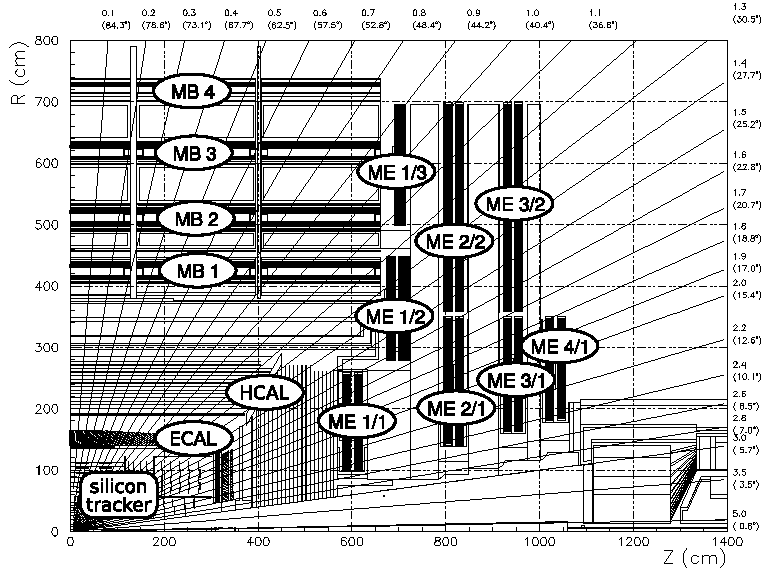
\includegraphics[height=\linewidth, angle=90]{plots/intro_geom/muon_system_labeled.pdf}

\caption{A quarter-view of CMS with labeled muon barrel (MB) and endcap (ME) stations. \label{fig:muon_system_labeled}}
\end{figure}

Barrel DT chambers have internal structure: superlayers
containing 4 layers each.  Stations 1--3 have 3 superlayers, the
middle one measuring a direction orthogonal to the outer
two.  Station 4 chambers have no middle superlayer (only superlayers~1
and 3).  Endcap CSCs contain 6 identical layers, each of which
measures both coordinates with intersecting cathode strips and anode
wires.

\subsection{Coordinate systems and conventions}

The Alignment Integration Frame, a coordinate system in which all
tracking systems are to be aligned, is defined by the 
tracker.  The origin of this system is the center of mass of the
tracker's detector elements~\cite{ref:tracker_alignment}, close to the
LHC interaction point, and oriented such that the $+z$ axis points
roughly along the beamline, to the west.  The $+y$ axis points
vertically upward, with $+x$ forming a right-handed coordinate system
by pointing south~\cite{ref:twikiCMSConventions}.  These same
coordinates can be expressed cylindrically, with $x$ and $y$ replaced
by $r = \sqrt{x^2 + y^2}$ and $\phi = \tan^{-1}(y/x)$.  The
curvilinear coordinate $r\phi$ is perpendicular to the beamline and
to rays from the beamline, and differentials of $r\phi$ are understood to
vary in $\phi$, not $r$ (so $d(r\phi)$ is equivalent to $r \, d\phi$).

Each muon chamber and layer has its own local coordinate system,
centered on the subdetector with local $z$ being perpendicular to the
measurement planes, and $+z$ points in the direction of decreasing
layer number.  The local $x$ axis roughly corresponds to global $r\phi$ (though for some chambers the direction is reversed),
and local $y$ forms a right-handed coordinate system.  In the absence
of misalignment, $y$ is parallel to the beamline for DT chambers and
radial for CSCs.

Layer/superlayer coordinate systems differ slightly from their parent
chambers.  The origin of each coordinate system is centered such that
$z=0$ lies on the layer and the average of layers in the superlayer, and
both layers and superlayers have small offsets in $x$ as well.  The
middle superlayer of DT chambers (superlayer~2) are rotated by 90$^\circ$ with
respect to the chamber coordinates, such that $x$ measurements in
these layers are $y$ positions in chamber coordinates.  Internal
alignments of layers introduce additional corrections.

Cathode strips in CSC layers fan radially from the beamline,
intersected by anode wires.  The strips measure a coordinate
perpendicular to their orientation, which in the absence of
misalignment coincides with global $r\phi$ throughout the chamber.  We
find ``local $r\phi$,'' or local $x$ times the cosine of the strip
angle, to be a more convenient coordinate than $x$ for CSCs.  This is
because local $r\phi$ is determined purely by high-precision strip
measurements, avoiding input from the groups of ganged wires which
would introduce a complicated and large-scale (cm) granularity to the
residuals distributions.

We describe the orientations of chambers and layers with $\phi_x$,
$\phi_y$, and $\phi_z$, where each is a right-hand rotation around the
corresponding coordinate axis.  The 3-D rotation is the following
composition:
\begin{equation}
\left(\begin{array}{c c c}
1 & 0 & 0 \\
0 & \cos\phi_x & \sin\phi_x \\
0 & -\sin\phi_x & \cos\phi_x
\end{array}\right) \cdot 
\left(\begin{array}{c c c}
\cos\phi_y & 0 & -\sin\phi_y \\
0 & 1 & 0 \\
\sin\phi_y & 0 & \cos\phi_y
\end{array}\right) \cdot
\left(\begin{array}{c c c}
\cos\phi_z & \sin\phi_z & 0 \\
-\sin\phi_z & \cos\phi_z & 0 \\
0 & 0 & 1
\end{array}\right)\mbox{.}
\end{equation}



%---------------------------------------------------------------------
\section{Local DT Alignment}
\label{sec:localdt}
This section describes the alignment of layers and superlayers within
DT chambers, using local information only.  Tracking data are combined
with physical measurements performed when the chambers were
constructed to resolve ambiguities between alignment and
track-fitting.  The chamber geometry obtained by these methods is an
important part of the global alignment described in a later section.

\subsection{Algorithm for General DT Layer Alignment}
\label{sec:standdt_general}

The tracks and physical survey data were merged into a consistent
geometry with a method based on the Millepede algorithm of
V.~Blobel~\cite{ref:Millepede}.  The basic idea behind this algorithm is
to define a $\chi^2$ with contributions from all sources: alignment,
track residuals, and survey residuals, and then minimize the $\chi^2$,
allowing all parameters to float.

Alignment corrections are represented by a vector with 6 parameters
per alignable (layers, superlayers, and in a later section, the
chambers themselves).  These are $\delta_x^i$, $\delta_y^i$,
$\delta_z^i$, $\delta_{\phi_x}^i$, $\delta_{\phi_y}^i$, and
$\delta_{\phi_z}^i$ with $i$ indexing the alignables.  Varying the
alignment affects residuals, the difference between experimental hits and fitted track
points.  Layers and superlayers measure hit positions in only one
dimension, so the effect of geometric corrections on residuals (${\Delta
x^i_j}^{\mbox{\scriptsize \, geom}}$ on alignable $i$ and track $j$) can
be related to alignment parameters through the following matrix:
\begin{equation}
\left(\begin{array}{c} 
{\Delta x^i_j}^{\mbox{\scriptsize \, geom}} \\
\end{array}\right) = 
\left(\begin{array}{c c c c c c}
-1 & 0 & \frac{dx}{dz} & -y\frac{dx}{dz} & x\frac{dx}{dz} & -y  \\
\end{array}\right)\cdot
\left(\begin{array}{c} 
\delta_x^i \\
\delta_y^i \\
\delta_z^i \\
\delta_{\phi_x}^i \\
\delta_{\phi_y}^i \\
\delta_{\phi_z}^i \\
\end{array}\right)
\label{eqn:dtstand_alignparams}
\end{equation}
for each alignable (where $y$ and $\frac{dx}{dz}$ are the track's $y$ position
and $x$ slope with respect to $z$, in the layer's coordinate system).
Tracks are most sensitive to $\delta_x$, and they have no sensitivity
to $\delta_y$ because the term connecting it to ${\Delta
x}^{\mbox{\scriptsize geom}}$ is zero.  We will henceforth denote the
vector of all alignment parameters as $\vec{\delta}$, and the matrix
connecting them to $\Delta x^{\mbox{\scriptsize geom}}$ as $A$ (the index $i$
is internal).  Expanding equation~\ref{eqn:dtstand_alignparams} to cover all alignables,
\begin{equation}
\left(\begin{array}{c} 
{\Delta x_j}^{\mbox{\scriptsize geom}} \\
\end{array}\right) = A \cdot \vec{\delta} \mbox{.}
\end{equation}

Track-fitting is part of the global minimization, so we must include a
term corresponding to variation the track parameters.  We parameterize
tracks inside of DT chambers as straight lines ($x_0$, $y_0$,
$\frac{dx}{dz}$ and $\frac{dy}{dz}$), since magnetic field lines
mainly follow the yokes between chambers, leaving negligible magnetic
field in the chambers themselves.  The effect of small corrections in
the track parameters on residuals ${\Delta
x^i_j}^{\mbox{\scriptsize \, track}}$ is also linear, and may be
represented by a matrix multiplying the track parameter corrections
\begin{equation}
\left(\begin{array}{c}
{\Delta x^i_j}^{\mbox{\scriptsize \, track}} \\
{\Delta y^i_j}^{\mbox{\scriptsize \, track}} \\
\end{array}\right) =
\left(\begin{array}{c c c c}
1 & 0 & z_i & 0 \\
0 & 1 & 0 & z_i \\
\end{array}\right)\cdot
\left(\begin{array}{c}
{\delta_{x_0}}_j \\
{\delta_{y_0}}_j \\
{\delta_{\frac{dx}{dz}}}_j \\
{\delta_{\frac{dy}{dz}}}_j \\
\end{array}\right)
\label{eqn:dtstand_trackparams}
\end{equation}
in the chamber's coordinate system.  (As a reminder, one-dimensional
$x$ positions in layer coordinates transform to $(0,\mbox{ }x)$ in
two-dimensional chamber coordinates for superlayer~2 and $(x,\mbox{
}0)$ for superlayers~1 and 3, in the absence of alignment
corrections.)  We will denote the corrections to the track parameters
as $\delta \vec{p_j}$ and the matrix connecting them to
$x^{\mbox{\scriptsize track}}$ as $B_j$, such that
Equation~\ref{eqn:dtstand_trackparams} becomes
\begin{equation}
\left(\begin{array}{c}
{\Delta x^i_j}^{\mbox{\scriptsize \, track}} \\
{\Delta y^i_j}^{\mbox{\scriptsize \, track}} \\
\end{array}\right) = B_j \cdot \delta \vec{p_j} \mbox{.}
\end{equation}

The observed residuals $\Delta \vec{x}$ are
\begin{equation}
\Delta \vec{x} = \Delta \vec{x}^{\mbox{\scriptsize \, geom}} + \Delta
\vec{x}^{\mbox{\scriptsize \, track}}
+ \Delta \vec{x}^{\mbox{\scriptsize \, meas}}
\end{equation}
where $\Delta \vec{x}^{\mbox{\scriptsize \, meas}}$ is a random
contribution from measurement error, assumed to be symmetric.  We can
now construct a $\chi^2$ which is minimized when tracks and chamber
geometry are mutually consistent:
\begin{equation}
{\chi^2}^{\mbox{\scriptsize \, track-based}} = \sum_j \left(\Delta \vec{x} - A \cdot \vec{\delta} - B_j \cdot \delta \vec{p_j} \right)^T \, \left({\sigma_{\mbox{\scriptsize resid}_{\mbox{\scriptsize $i$}}}}^2\right)^{-1} \, \left(\Delta \vec{x} - A \cdot \vec{\delta} - B_j \cdot \delta \vec{p_j} \right)
\label{eqn:chi2millepede}
\end{equation}
where ${\sigma_{\mbox{\scriptsize resid}_{\mbox{\scriptsize $i$}}}}^2$
is the covariance matrix of hits (no uncertainty in our track model).
However, ${\chi^2}^{\mbox{\scriptsize \, track-based}}$ cannot be
minimized: the system has more degrees of freedom than
constraints.  Consider, for instance, shearing all layers linearly in
$x$; this non-rigid deformation of the chamber leaves
${\chi^2}^{\mbox{\scriptsize \, track-based}}$ invariant because
fitted tracks compensate with $\frac{dx}{dz}$.  We therefore must
augment it with external data to yield a meaningful alignment.

\subsubsection{Quality Control Measurements}

As the DT chambers were being built, the positions of the wire
end-pins were measured and recorded~\cite{ref:QC}.  Local $\delta_x^i$
corrections can be determined from an average of the measurements over
layers.  Typical (RMS) corrections are 100~$\mu$m, with an uncertainty of 30--40~$\mu$m.  These measurements only constrain the
relative positions of layers within each superlayer, not the
superlayers relative to one another, because each superlayer was built
separately.

\subsubsection{Photogrammetry Measurements}

After superlayers were assembled into chambers, the position and
orientation of the superlayers were measured by photogrammetry (a
photograph of reflective targets at known points on the superlayer, in
a coordinate system defined by references at their
corners~\cite{ref:Survey}).  These measurements constrain superlayers
relative to one another, but not the layers inside).

Typical corrections are 200~$\mu$m for $\delta_x$ and $\delta_y$, with
150~$\mu$rad for rotations.  The $\delta_z$ corrections were 1--1.5~mm
because of a layer of glue not included in the design description.  We
take special care to cross-check these $\delta_z$ parameters
independently with tracks before applying the correction.

\subsubsection{Combination}

To include survey measurements into the global alignment fit, we need
a term to describe the effect of alignment corrections
$\vec{\delta^i}$ on the positions of the survey's control points
(nominally at $x_k$, $y_k$, $z_k$).  This term is
\begin{equation}
{\Delta \vec{x^i_k}}^{\mbox{\scriptsize \, points}} =
\left(\begin{array}{c c c c c c}
1 & 0 & 0 & y_k & z_k & 0 \\
0 & 1 & 0 & -x_k & 0 & z_k \\
0 & 0 & 1 & 0 & -x_k & -y_k \\
\end{array}\right) \cdot
\vec{\delta^i}
\end{equation}
and we denote the matrix for all control points on all alignables as
$C$ (alignable index $i$ and survey point index $k$ are internal).
This matrix is constructed in such a way as to internally account for
the fact that some measurements are relative differences, rather than
absolute coordinates.  The $\chi^2$ of survey measurements is
\begin{equation}
{\chi^2}^{\mbox{\scriptsize \, survey}} = \left({\Delta \vec{x}}^{\mbox{\scriptsize \, survey}} - C \cdot \vec{\delta} \right)^T \, \left({\sigma_{\mbox{\scriptsize survey}}}^2\right)^{-1} \, \left({\Delta \vec{x}}^{\mbox{\scriptsize \, survey}} - C \cdot \vec{\delta} \right)
\end{equation}
where ${\Delta \vec{x}}^{\mbox{\scriptsize \, survey}}$ are the measured positions
from survey and photogrammetry, and ${\sigma_{\mbox{\scriptsize
survey}}}^2$ is their covariance matrix.

Finally, the global chamber position can never be determined from
local information, so translations and rotations of the whole chamber
are fixed to zero with Lagrange multipliers $f(\lambda)$.  The final
$\chi^2$ is
\begin{equation}
\chi^2 = {\chi^2}^{\mbox{\scriptsize \, track-based}} +
{\chi^2}^{\mbox{\scriptsize \, survey}} + f(\lambda) \mbox{,}
\end{equation}
which we minimize by a straight-forward numerical inversion of the
derivatives matrix, as the number of alignable parameters is not
large.

\subsection{Independent Cross-Check of $\delta_z$}
\label{sec:standdt_independent}

As explained above, the largest correction from the design geometry
was in the superlayers' $z$ coordinates, due to a layer of glue not
included in the design description.  To cross-check these
photogrammetry measurements, we determined them from an independent
track-based measurement.

As the displacement under study is between superlayers, track segments
fitted in each superlayer individually are not affected by the
correction.  We can therefore simplify the $\chi^2$ by re-defining
residuals in this case as a difference between single-superlayer track
segments (superlayers~1 and 3 only), extrapolated to a common plane.
The $B_j$ matrix vanishes, leaving us with
\begin{equation}
\chi^2 = \sum_j \left(\Delta \vec{x} - A \cdot \vec{\delta}\right)^T \, \left({\sigma_{\mbox{\scriptsize resid}}}^2\right)^{-1} \, \left(\Delta \vec{x} - A \cdot \vec{\delta}\right)
\end{equation}
where ${\sigma_{\mbox{\scriptsize resid}}}^2$ is the covariance matrix
for these new residuals.  We further simplify the alignment by only
allowing $\delta_x$, $\delta_z$, and $\delta_{\phi_y}$ to float, as
these are the parameters that can be determined purely from track
segments in one-dimensional measurement devices.  The alignment
derivatives matrix $A$ for each chamber is reduced to
\begin{equation}
\left(\begin{array}{c} 
{\Delta x^i_j}^{\mbox{\scriptsize \, geom}} \\
\end{array}\right) = 
\left(\begin{array}{c c c c c c}
-1 & \frac{dx}{dz} & x\frac{dx}{dz}  \\
\end{array}\right)\cdot
\left(\begin{array}{c} 
\delta_x^i \\
\delta_z^i \\
\delta_{\phi_y}^i \\
\end{array}\right) \mbox{.}
\end{equation}
A geometric interpretation of the $\delta_z$ term is given in
Figure~\ref{fig:extrapolation}.  With these simplifications, it is
possible to align superlayers purely with track-based data.

\begin{figure}
  \begin{center}
  \subfigure[Interpretation of $\Delta x^{\mbox{\scriptsize geom}} = \frac{dx}{dz} \delta_z$.]{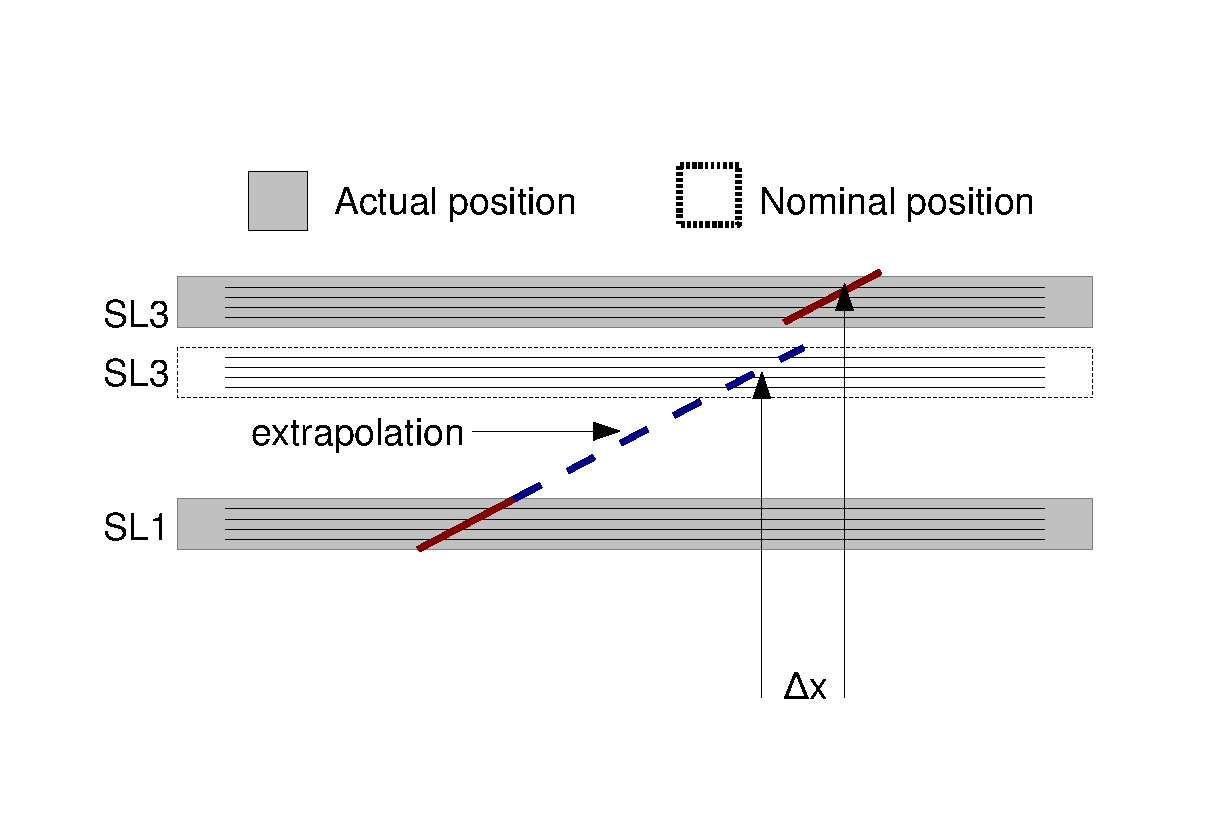
\includegraphics[width=0.45\linewidth]{plots/standalone_dt_alignment/internalThickness.pdf} \label{fig:extrapolationa}}
  \subfigure[A typical $\delta_z$ displacement, observed as a slope in $\Delta x$ versus $\frac{dx}{dz}$.]{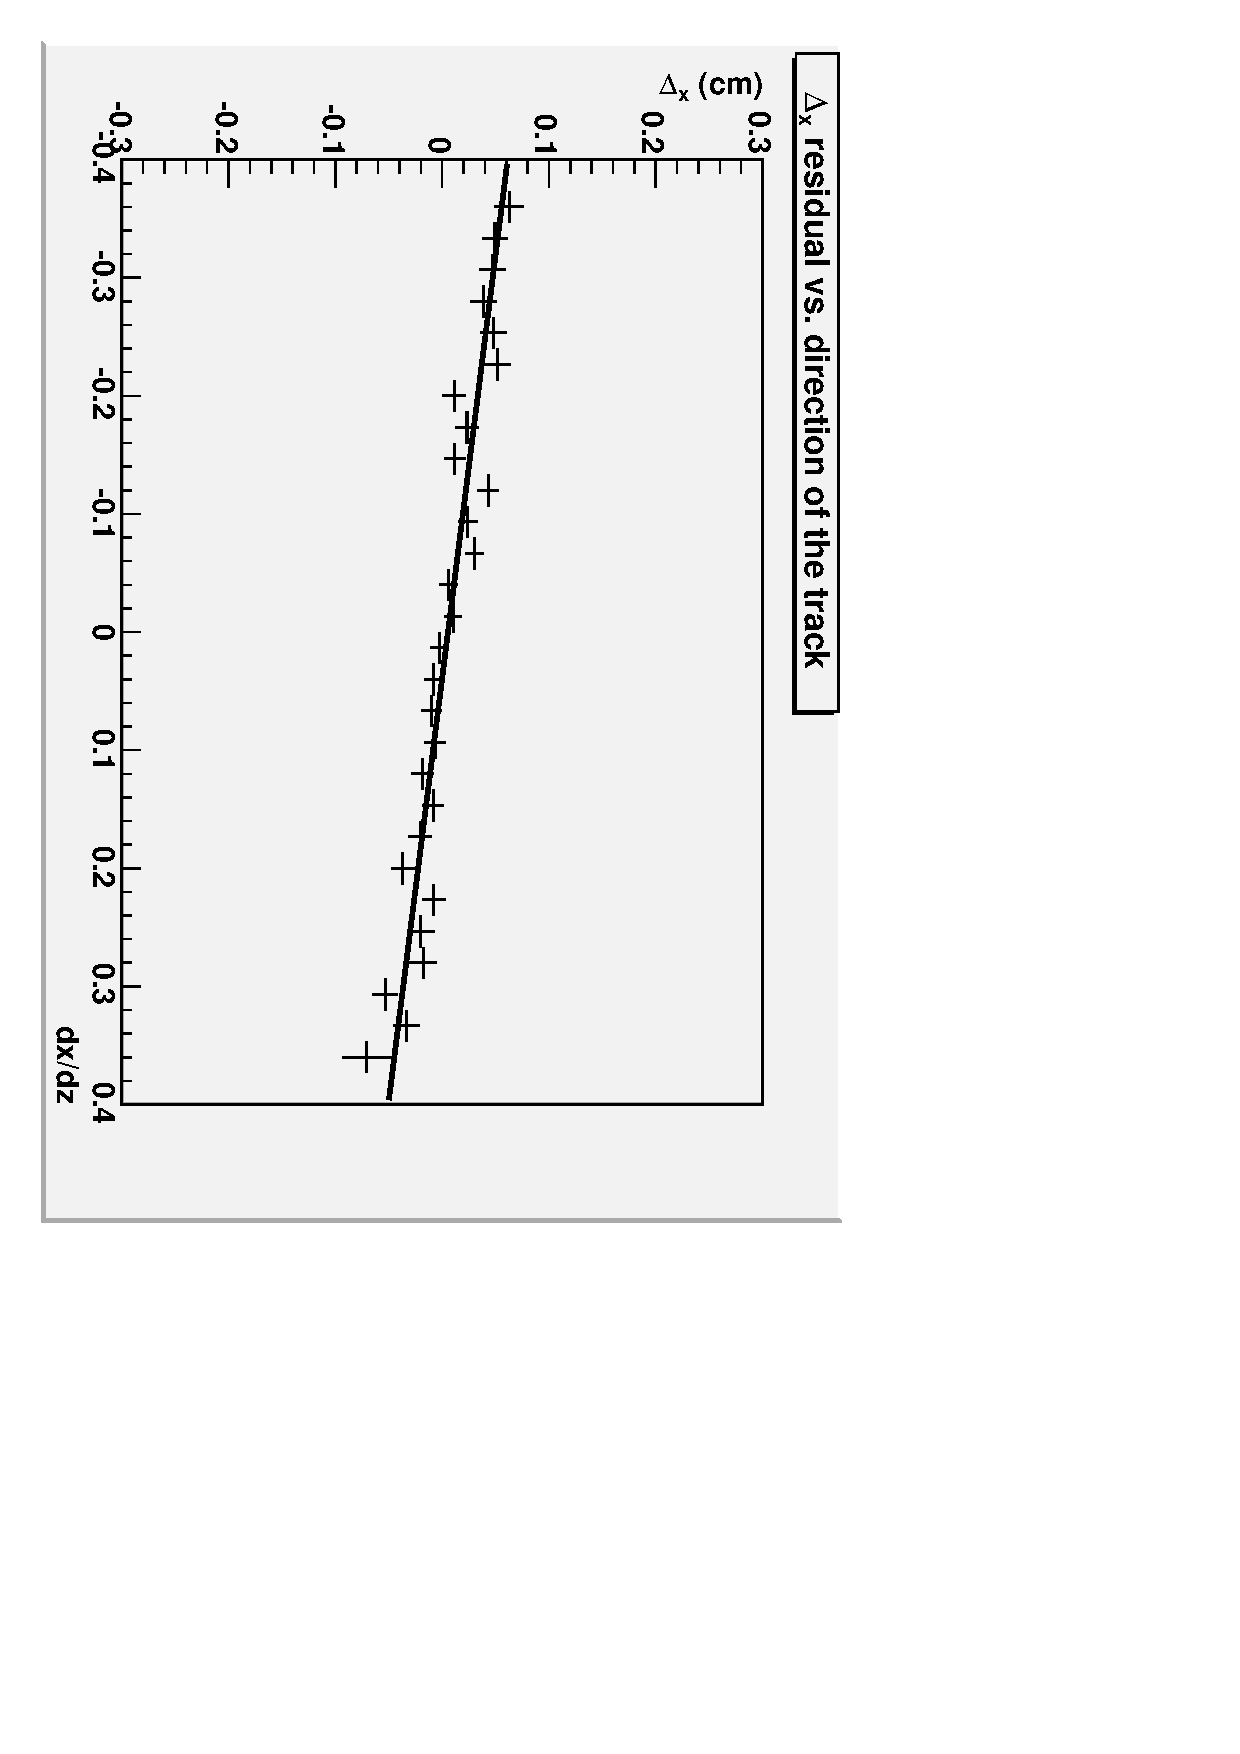
\includegraphics[height=0.45\linewidth, angle=90]{plots/standalone_dt_alignment/xphi014.pdf} \label{fig:slopetracks}}
  \end{center}
  \caption{Measuring $\delta_z$ with tracks only. \label{fig:extrapolation}}
\end{figure}

The $\delta_z$ corrections from survey (photogrammetry), this
track-based method, and their differences are plotted in
Figure~\ref{fig:surveyvstracks}, revealing independent agreement in
non-negligible corrections.  Typical discrepancies are 580~$\mu$m (RMS
and Gaussian width) in $\delta_z$, while the size of the corrections
range from 1 to 2~mm (thicker glue was used in station~1).  The
$\delta_x$ and $\delta_{\phi_y}$ corrections were also in agreement,
but they were negligible (80~$\mu$m and 50~$\mu$rad, respectively).

\begin{figure}
  \begin{center}
  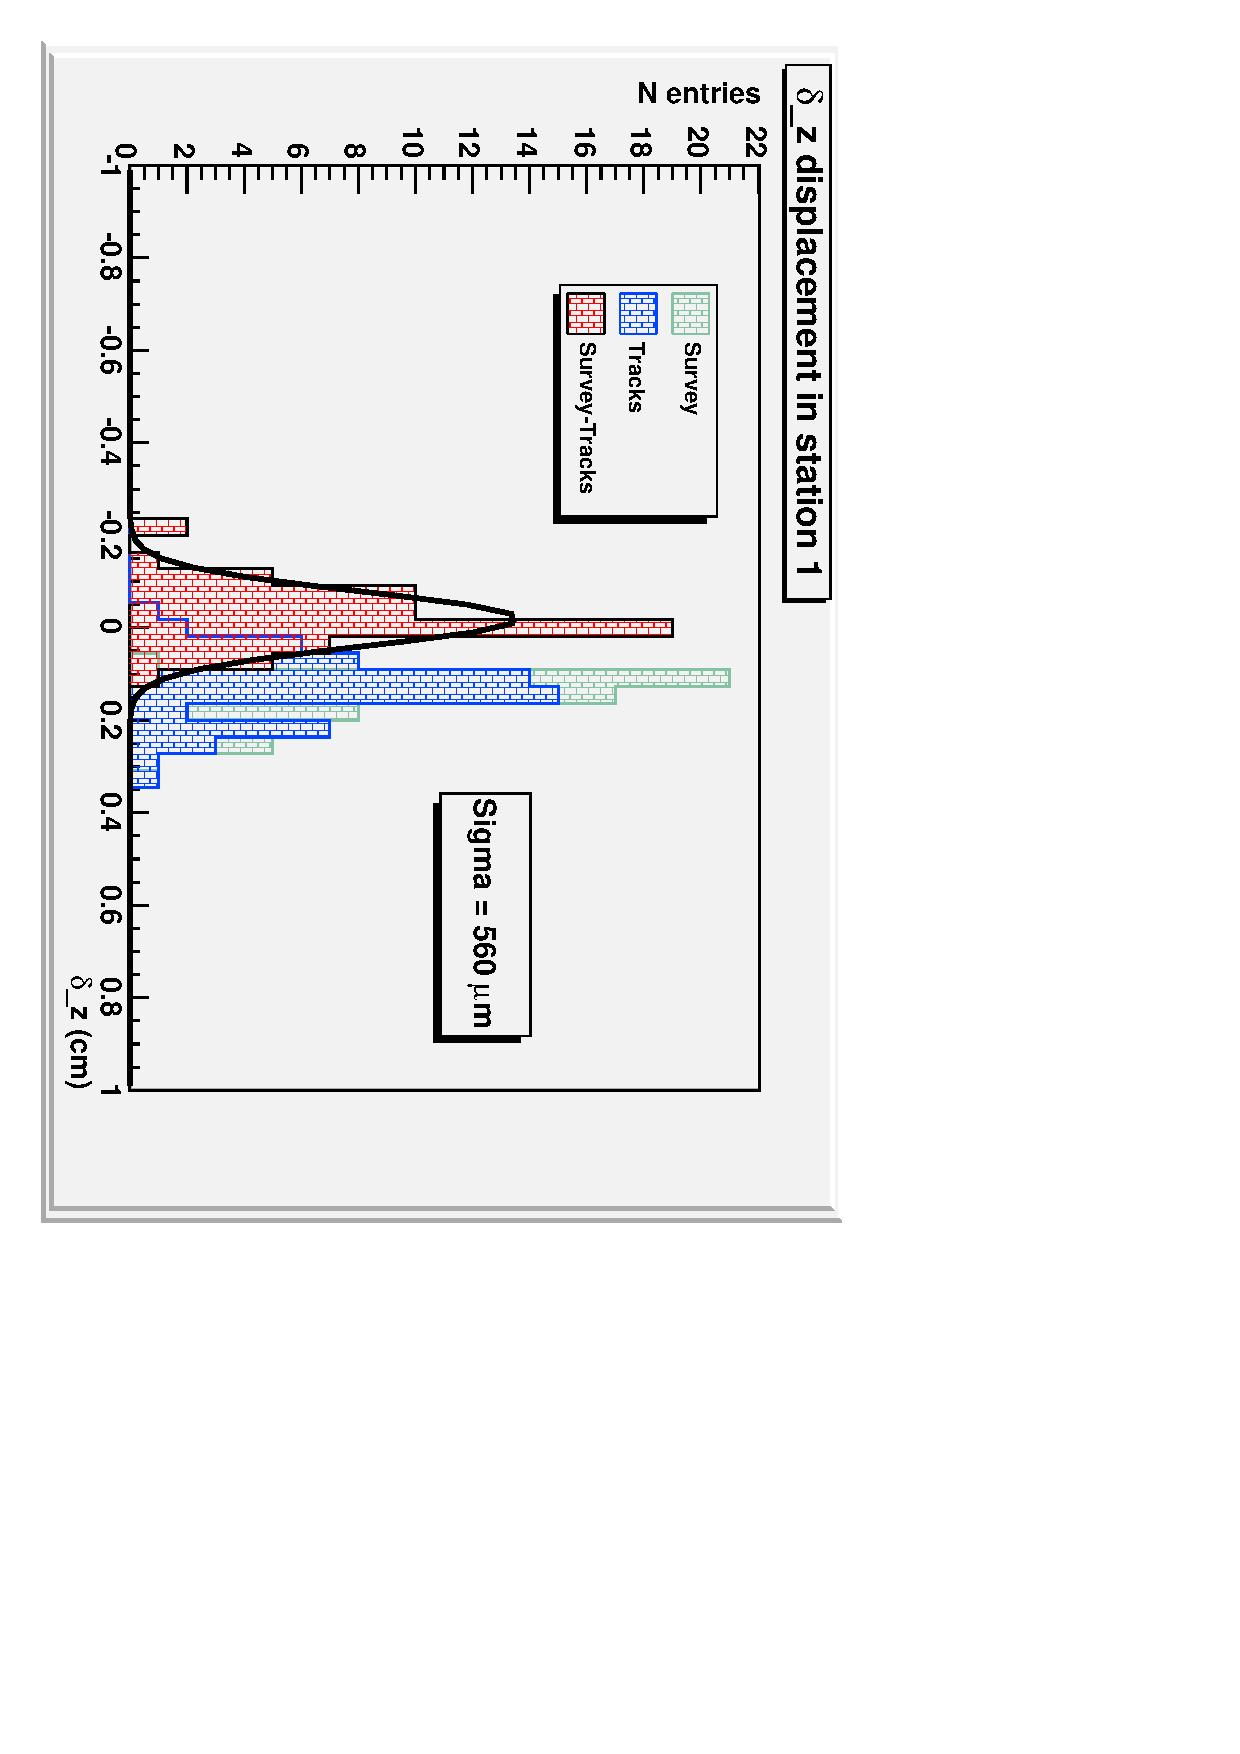
\includegraphics[height=\linewidth, angle=90]{plots/standalone_dt_alignment/DiffereceancesAllSurveyTracksST1.pdf}
  \end{center}
  \caption{Comparison of survey and track-based alignment of $\delta_z$ of superlayers in DT chambers.  Each entry in this histogram is a $\delta_z$ measurement for one chamber, with the three distributions corresponding to survey (photogrammetry) only, tracks only, and the chamber-by-chamber difference between survey and tracks. \label{fig:surveyvstracks}}
\end{figure}

The internal DT geometry used in the global alignment was determined
by the combined fit described in subsection~\ref{sec:standdt_general}
with $\delta_z$ fixed, followed by corrections from the tracks-only
method described above.  It therefore incorporates all available
information except that which is reserved for cross-checking the
sources.


%---------------------------------------------------------------------
\section{Local CSC Alignment}
\label{sec:localcsc}
The CSCs in the muon endcap were designed to overlap slightly along
their edges, such that a track passing through the narrow ``overlap
regions'' would be observed by both of the neighboring chambers,
without scattering volumes in between or propagation over large
distances.  These tracks can therefore measure the relative alignment
of the pairs of chambers they connect with high precision.  All endcap
rings except for ME1/3 are connected in this way by overlaps.  In this
section, we will describe a method to align CSCs within each ring with
only a small sample of tracks and demonstrate the accuracy of the
method by comparing its results with an independent measurement.

\subsection{Overlap Method Algorithm} 

The basic strategy is to measure differences in alignment parameters
for pairs of chambers and then propagate alignment corrections azimuthally around
the ring by solving a system of equations.  Relative alignment
corrections between overlapping neighboring chambers $i$ and $i+1$ are derived
from the consistency of track segments with a single, straight line.

At each interface between two overlapping chambers, we fit hits in the 6 layers of
each chamber to straight lines $r\phi_i(z) = a_i + b_i z$ and
$r\phi_{i+1}(z) = a_{i+1} + b_{i+1} z$ in a shared coordinate system
and then propagate these segments to a plane equidistant between the
two chambers (at $z=0$).  The position-matching residual on the
plane is $\Delta a = a_i - a_{i+1}$ and the angle-matching residual
is $\Delta b = b_i - b_{i+1}$.  The overlap region is a thin strip
spanning the chamber only along the $y$ dimension, so we can consider
fitting these residuals as a function of the track's $y$ intersection
with the plane of comparison (a linear fit of linear track-fits).
We therefore have access to four types of residuals:
\begin{itemize}
\item $\Delta a(y=0)$: the relative $\delta_{r\phi}$
correction in position along a circle centered on the beamline,
\item $\Delta b(y=0)$: the relative $\delta_{\phi_y}$
angle between the two chambers,
\item $\frac{\partial}{\partial y} \Delta a(y)$: the relative $\delta_{\phi_z}$ angle,
\item $\frac{\partial}{\partial y} \Delta b(y)$: a non-rigid twist of the chambers.
\end{itemize}
We consider only the three alignment corrections ($\delta_{r\phi}$,
$\delta_{\phi_y}$, and $\delta_{\phi_z}$), presented graphically in
Figure~\ref{fig:overlaps_parameters}.

\begin{figure}
\subfigure[$\delta_{\phi_y}$ from $\Delta b(y=0)$]{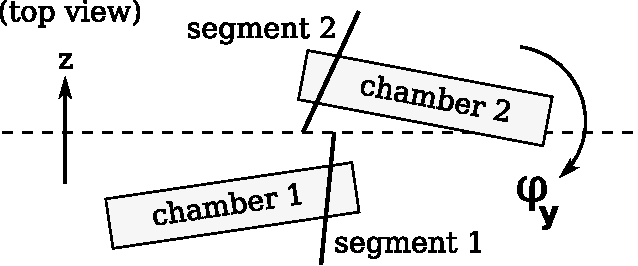
\includegraphics[width=0.33\linewidth]{plots/csc_overlaps_alignment/topview_1.pdf}} \hfill \subfigure[$\delta_{r\phi}$ from $\Delta a(y=0)$]{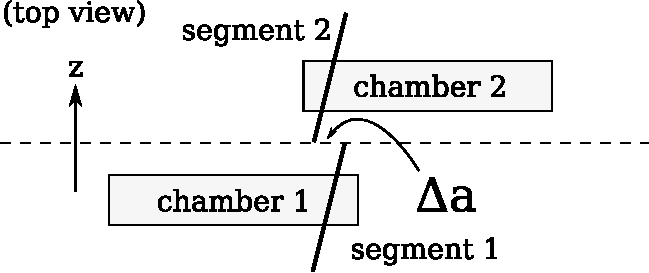
\includegraphics[width=0.33\linewidth]{plots/csc_overlaps_alignment/topview_2.pdf}} \hfill \subfigure[$\phi_z$ from $\frac{\partial}{\partial y} a(y)$]{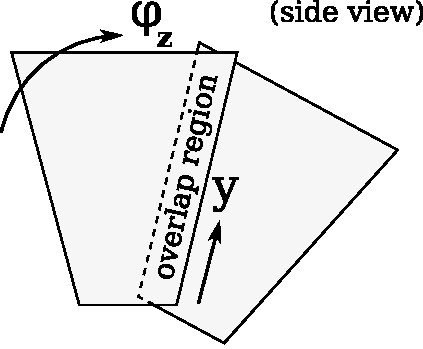
\includegraphics[width=0.18\linewidth]{plots/csc_overlaps_alignment/sideview.pdf}}
\caption{How three track parameters are determined from linear fits to $\Delta a(y)$ and $\Delta b(y)$, where $\Delta a$ and $\Delta b$ are the positions and slopes of track segments at a plane between the two CSCs.  \label{fig:overlaps_parameters}}
\end{figure}

While it is possible to resolve all three corrections at once, note
that $\delta_{\phi_y}$ is independent of the other two and
$\delta_{r\phi}$ is independent of $\delta_{\phi_z}$.  We can
therefore ignore dependencies if we align the parameters in the
following order: $\delta_{\phi_y}$, then $\delta_{r\phi}$, and then
$\delta_{\phi_z}$.

The problem of propagating alignment corrections around the ring is
identical for each of the three parameters, so we will present it only
once in an abstract way.  Label the mean of each residuals
distribution $\alpha_{i\mbox{\scriptsize, }i+1}$ (for each of the
three types of residuals under consideration) with $A_i$ and $A_{i+1}$
being the alignment corrections for the neighboring chambers
($\delta_{\phi_y}$, $\delta_{r\phi}$, or $\delta_{\phi_z}$).  Each
ring has $N$ = 18 or 36 chambers, so $i$ ranges from 1 to $N$ with the
convention that $N+1 = 1$ (to close the loop).

If we move chamber $i$ and $i+1$ by $A_i$ and $A_{i+1}$, the mean of
the residuals between them can be expected to change by $(A_i -
A_{i+1})$.  To optimize all of the residuals at once, we define a
$\chi^2$ as
\begin{equation}
\chi^2 = (\alpha_{12} - A_1 + A_2)^2 + (\alpha_{23} - A_2 + A_3)^2 + \ldots + (\alpha_{N1} - A_N + A_1)^2
\end{equation}
and minimize it by setting its derivatives to zero.  For example,
\begin{equation}
\frac{1}{2} \frac{\partial \chi^2}{\partial A_2} = (\alpha_{12} - A_1 + A_2) - (\alpha_{23} - A_2 + A_3) = 0 \mbox{.}
\end{equation}
A complete set of such equations, written in matrix form, looks like
the following:
\begin{equation}
\left(\begin{array}{c}
\alpha_{1,2} - \alpha_{N,1} \\
\alpha_{2,3} - \alpha_{1,2} \\
\vdots \\
\alpha_{(N-1),N} - \alpha_{(N-2),(N-1)} \\
\alpha_{N,1} - \alpha_{(N-1),N}
\end{array} \right)
=
\left(\begin{array}{r r r r r}
2 & -1 &  &  & -1 \\
-1 & 2 & -1 &  &  \\
 &  & \ddots & &  \\
 &  & -1 & 2 & -1 \\
-1 &  &  & -1 & 2
\end{array}\right)
\left(\begin{array}{c}
A_1 \\
A_2 \\
\vdots \\
A_{N-1} \\
A_N \\
\end{array} \right)\mbox{.}
\label{eqn:NbyNmatrix}
\end{equation}
To align all $N$ chambers, we need only invert this $N\times N$
matrix, and $N$ is small enough to be manageable.

Unfortunately, the matrix in Equation~\ref{eqn:NbyNmatrix} is singular
because a relative alignment procedure cannot determine the global
position of the whole system.  Rotating the whole ring rigidly by
adding the same constant to every $A_i$ would leave the $\chi^2$
invariant.  This is a flat direction in ($A_1$, $A_2$, \ldots\ $A_N$)
space, and it can be unflattened by preferring the corrections $A_i$
to be as small as possible.  We add the average of $A_i$
\begin{equation}
\left[ \frac{1}{N} \left(A_1 + A_2 + \ldots + A_N\right) \right]^2
\label{eqn:average}
\end{equation}
to the $\chi^2$ so that it will be minimized, and each derivative
equation becomes
\begin{equation}
\frac{1}{2} \frac{\partial \chi^2}{\partial A_i} = (\alpha_{i-1\mbox{\scriptsize, }i} - A_{i-1} + A_i) - (\alpha_{i\mbox{\scriptsize, }i+1} - A_i + A_{i+1}) + \frac{1}{N^2} \sum_{i=1}^N A_i = 0 \mbox{.}
\end{equation}
The right-hand-side of Equation~\ref{eqn:NbyNmatrix} becomes
\begin{equation}
\left[\left(\begin{array}{r r r r r}
2 & -1 &  &  & -1 \\
-1 & 2 & -1 &  &  \\
 & & \ddots & &  \\
 &  & -1 & 2 & -1 \\
-1 &  &  & -1 & 2
\end{array}\right)
+
\frac{1}{N^2}
\left(\begin{array}{r r r r r}
1 & 1 & \cdots &   & 1 \\
1 & 1 &   &   &   \\
\vdots &   & \ddots &   &   \\
  &   &   &   &   \\
1 &   &   &   & 1
\end{array}\right)
\right]
\left(\begin{array}{c}
A_1 \\
A_2 \\
\vdots \\
A_4 \\
A_5 \\
\end{array} \right)\mbox{.}
\label{eqn:solution}
\end{equation}
It has a unique solution in which the average of $A_i$ is exactly
zero.

The circular ring of chambers also provides an internal cross-check:
the closure
\begin{equation}
\sum_{i=1}^N \alpha_{i\mbox{\scriptsize, }i+1} - (A_i - A_{i+1}) = \sum_{i=1}^N \alpha_{i\mbox{\scriptsize, }i+1}
\end{equation}
must be zero.  The closure is independent of alignment, because all
$A_i$ terms cancel in the sum.  A non-zero closure would indicate an
incorrect circumference for the ring, either from our description of
the chamber widths or their radial distance from the beamline.  All
measured values of closure were consistent with zero.

This algorithm can be extended to align layers within the CSC
chambers, taking advantage of the two-chamber overlap to resolve
ambiguities between track-fitting and layer alignment in an isolated
chamber.  In the 2008 LHC beam-halo run, many layer measurements were
not statistically significant, with a precision of 50--100~$\mu$m, so
we do not present the results here.

\subsection{Monte Carlo Study}

The procedure was first applied to simulated beam-halo with
approximately the same number of events as the 2008 LHC run.  The
azimuthal and radial distributions are not exactly the same as in
data, as they are notoriously difficult to predict for a new
accelerator.  Starting from a misaligned detector, the procedure
re-aligned $\delta_{\phi_y}$ with about 1~mrad precision,
$\delta_{r\phi}$ with about 230~$\mu$m, and $\delta_{\phi_z}$ with
about 0.25~mrad, by comparison with the true positions of the
chambers, known in simulation.  Figure~\ref{fig:overlaps_mc}
shows histograms of the differences between aligned values of the
parameters and their true values.

\begin{figure}
\subfigure[$\delta_{\phi_y}$ precision is $\sim$1~mrad]{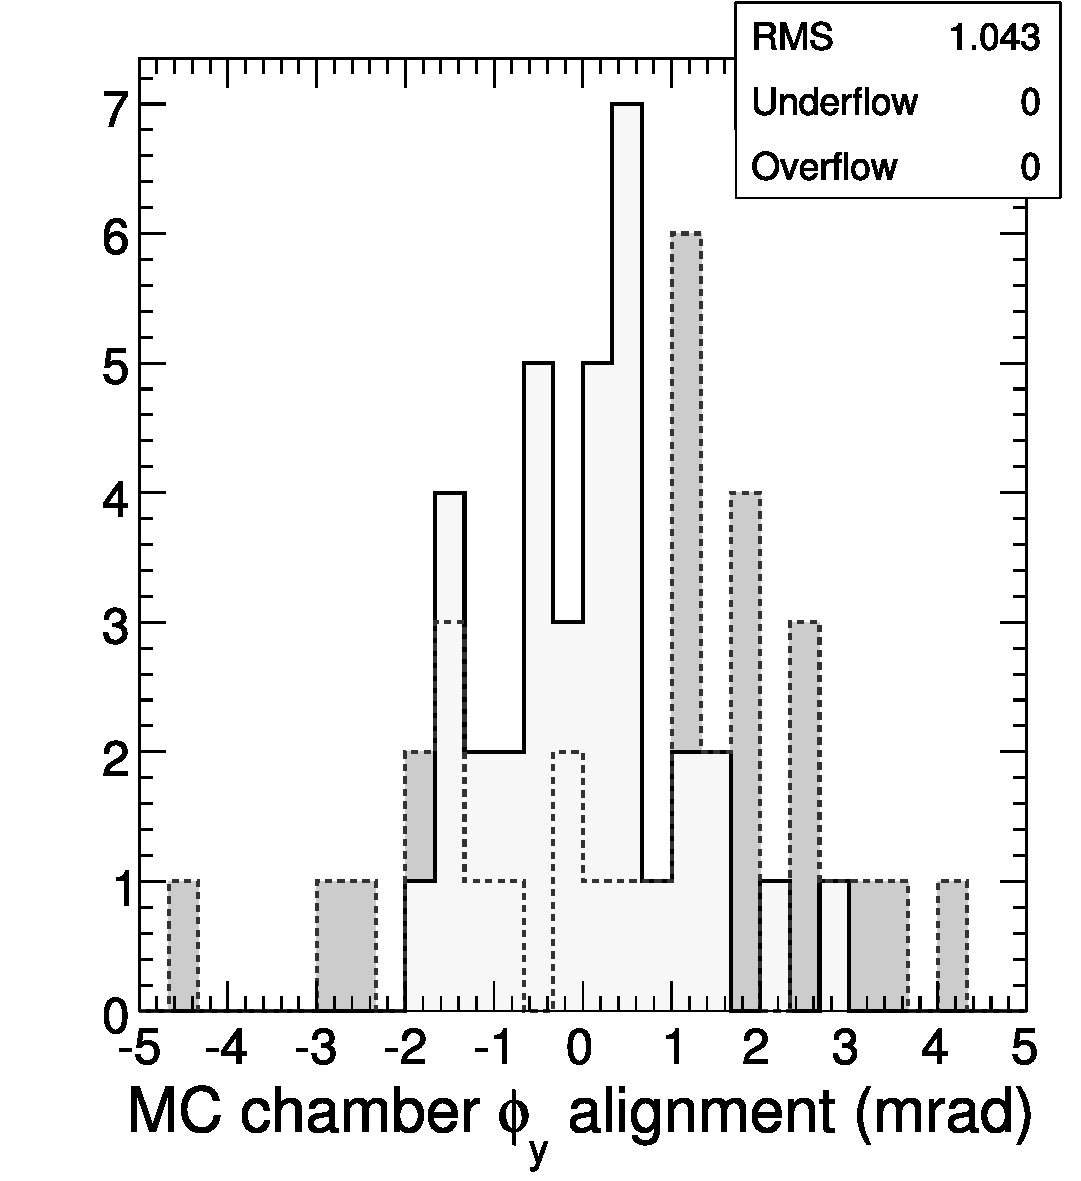
\includegraphics[width=0.3\linewidth]{plots/csc_overlaps_alignment/mcchamber_phiy.pdf}} \hfill \subfigure[$\delta_{r\phi}$ precision is $\sim$230~$\mu$m]{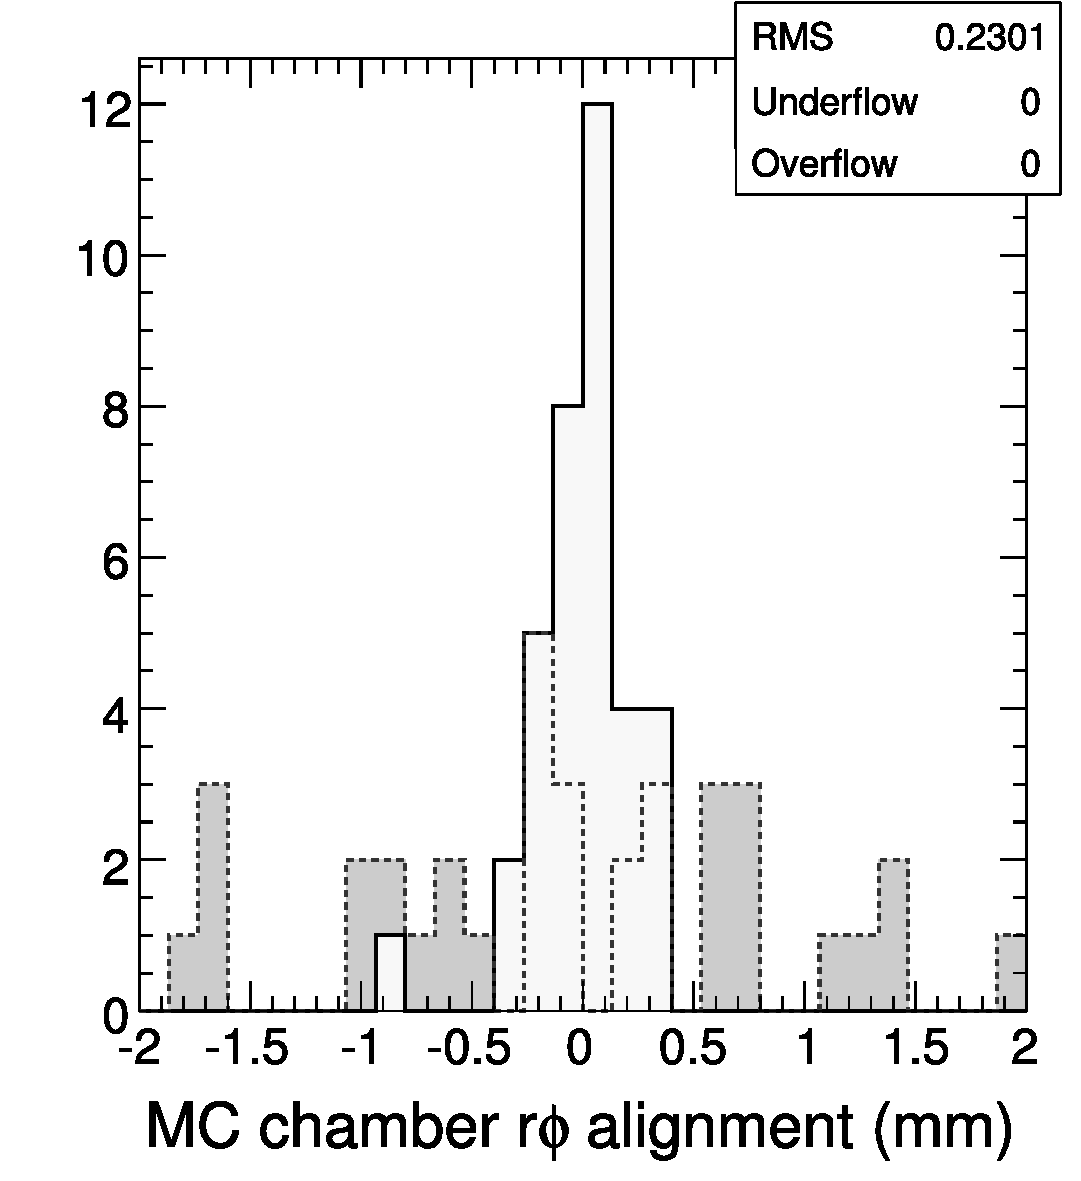
\includegraphics[width=0.3\linewidth]{plots/csc_overlaps_alignment/mcchamber_rphi.pdf}} \hfill \subfigure[$\delta_{\phi_z}$ precision is $\sim$0.25~mrad]{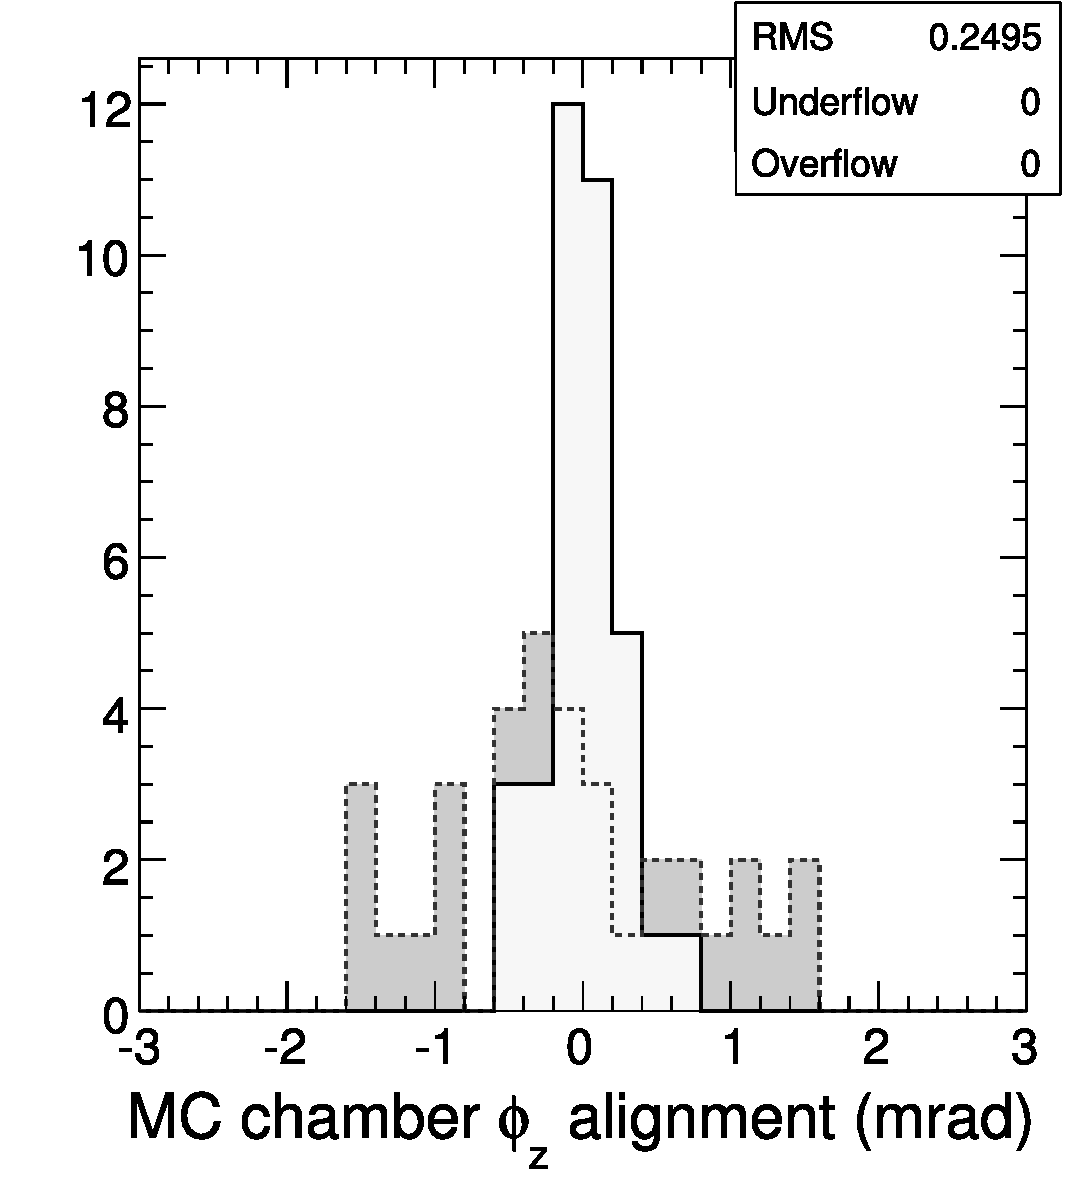
\includegraphics[width=0.3\linewidth]{plots/csc_overlaps_alignment/mcchamber_phiz.pdf}} \hfill
\caption{Comparison of CSC alignment parameters with their true values before (dark) and after (light) a simulated beam-halo alignment with similar statistics to the 2008 LHC run. \label{fig:overlaps_mc}}
\end{figure}

\subsection{Alignment Results}

In September of 2008, protons circulated in beam-2 of the LHC tunnel
for 9~minutes, and enough data were collected to test the CSC Overlaps
procedure.  More beam-halo muons illuminated the inner rings (ring~1)
of the minus side of the endcap because beam-halo muons tend to be close to
the beamline and beam-2 passed through CMS in the direction from $-z$ toward $+z$.  At
that time, all chambers in ME$-$2/1 and ME$-$3/1 were operational, so
we aligned them with the CSC Overlaps algorithm.

To verify the aligned positions, we compare them with photogrammetry
measurements.  Each chamber has two reflective alignment targets whose
positions can be measured with 300~$\mu$m precision by photographing
them in a strong light.  From these, $\delta_{r\phi}$ and
$\delta_{\phi_z}$ corrections (relative to the design geometry) can be
computed with $\mbox{(300~$\mu$m)}/\sqrt{2} = 210$~$\mu$m and
$\mbox{(300~$\mu$m)} \cdot \sqrt{2} / \ell = 0.23$~mrad precision,
respectively (where $\ell$ is half the distance between photogrammetry
targets, about 1.9~m in this case).  Errors from $\phi_y$
misalignments are negligible in these transformations.  The
photogrammetry and track-based measurements were both taken with the
CMS solenoid turned off.  (The solenoid's field is strong enough to
move the chambers, invalidating the measurement.)  Unlike
photogrammetry, the track-based measurement can also be performed with
the solenoid on, though no such data were taken while LHC beam-halo muons
could be collected.

In Figure~\ref{fig:overlaps_data1}, the track-based and photogrammetry
corrections to ideal geometry are presented.  Both yield significant
deviations from zero, yet agree rather well.  We plot the same
data as histograms of differences between track-based and
photogrammetry measurements in Figure~\ref{fig:overlaps_data2}, and
observe that the widths of these distributions are 340~$\mu$m and
0.42~mrad.  Subtracting the
photogrammetry uncertainties in quadrature from standard deviations
observed in the plots,
\begin{eqnarray}
\mbox{track-based $\delta_{r\phi}$ accuracy} &=& \sqrt{(\mbox{340~$\mu$m})^2 - (\mbox{210~$\mu$m})^2} = \mbox{270~$\mu$m} \\
\mbox{track-based $\phi_z$ accuracy} &=& \sqrt{(\mbox{0.42~mrad})^2 - (\mbox{0.23~mrad})^2} = \mbox{0.35~mrad,}
\end{eqnarray}
in rough agreement with the simulation's prediction and close to the
scale of the intrinsic hit resolution of the detectors (116~$\mu$m).  Assuming that
the errors are statistical, an hour or more of similar tracks would
yield an alignment that is more precise than the intrinsic hit resolution.

\begin{figure}
\begin{center}
\begin{minipage}{\linewidth}
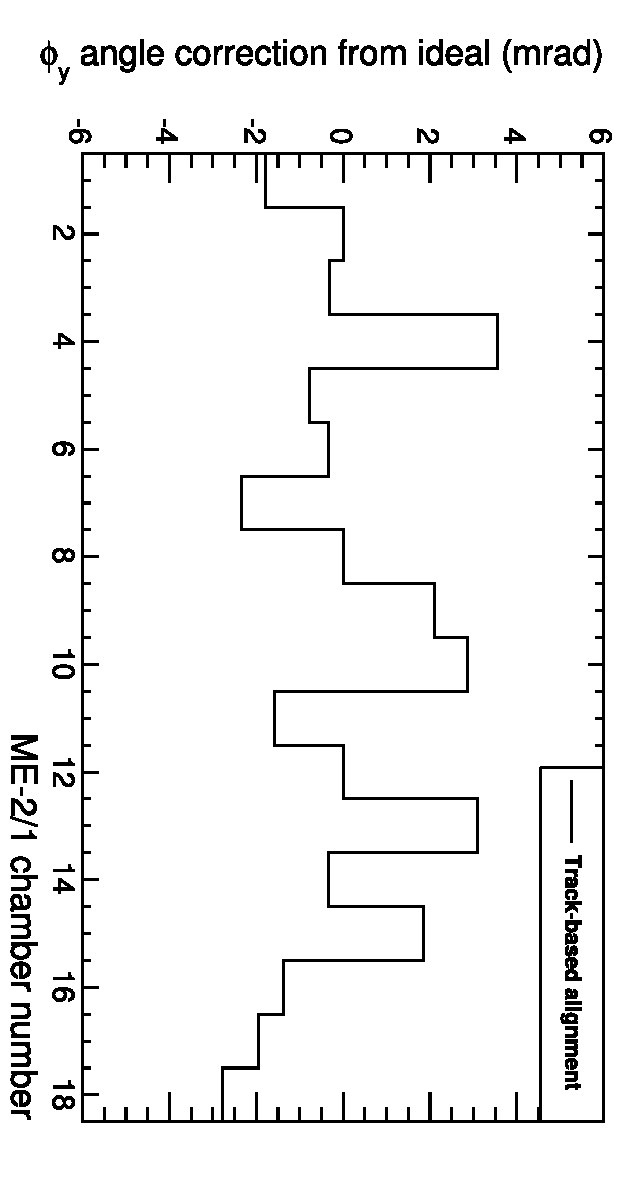
\includegraphics[height=0.48\linewidth, angle=90]{plots/csc_overlaps_alignment/compare_m21_phiy.pdf} 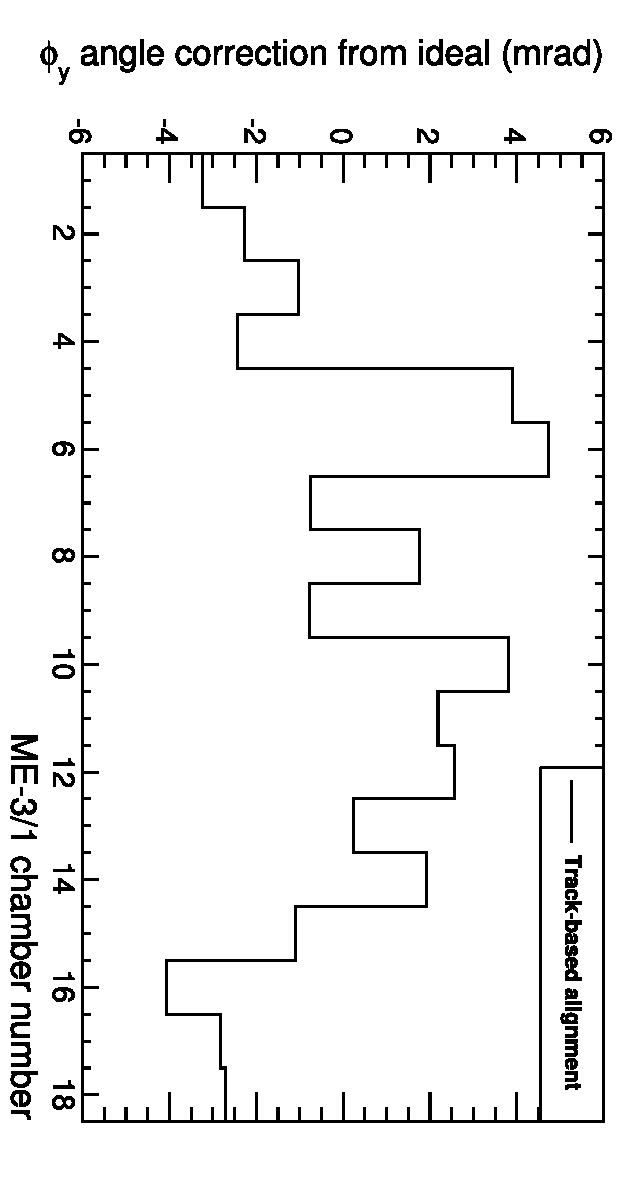
\includegraphics[height=0.48\linewidth, angle=90]{plots/csc_overlaps_alignment/compare_m31_phiy.pdf}

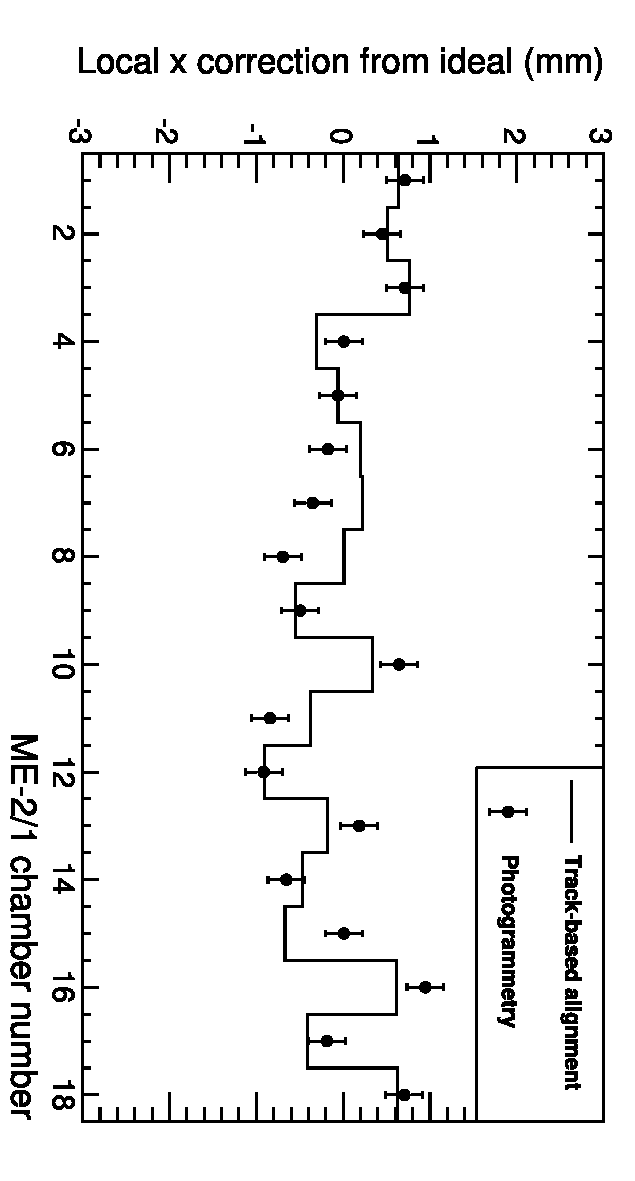
\includegraphics[height=0.48\linewidth, angle=90]{plots/csc_overlaps_alignment/compare_m21_x.pdf} 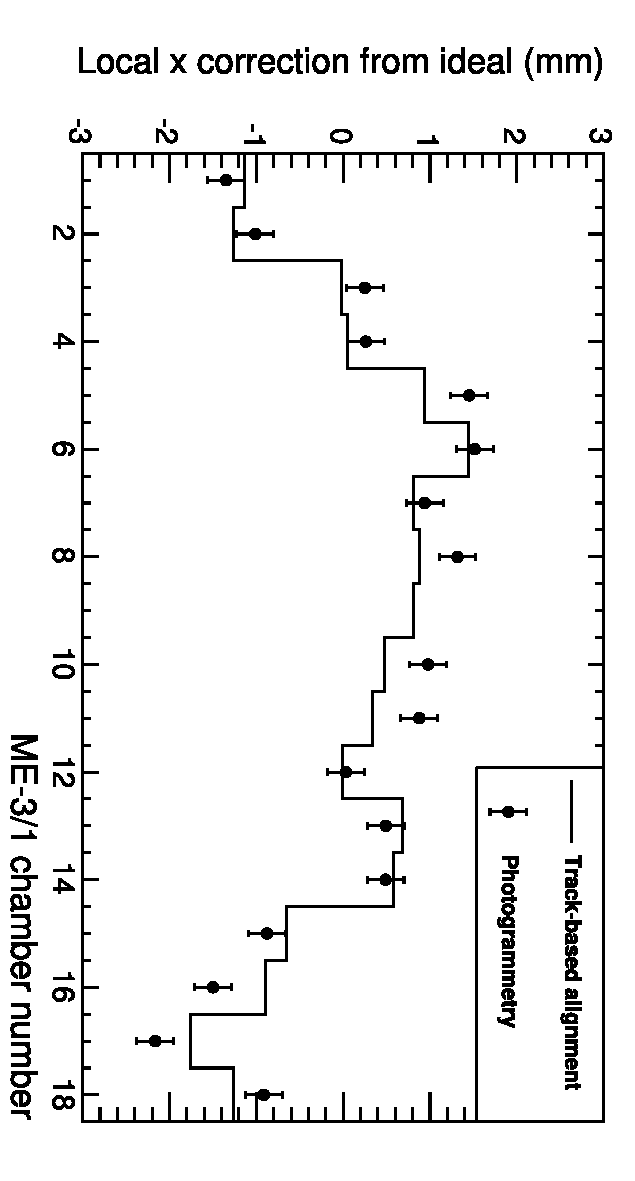
\includegraphics[height=0.48\linewidth, angle=90]{plots/csc_overlaps_alignment/compare_m31_x.pdf}

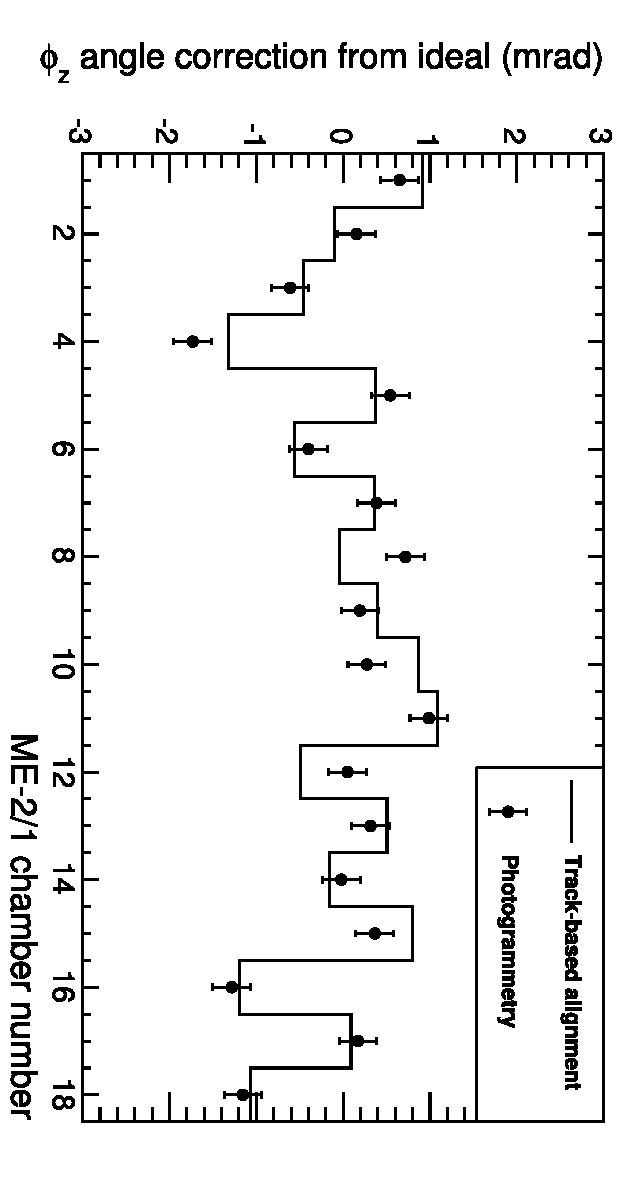
\includegraphics[height=0.48\linewidth, angle=90]{plots/csc_overlaps_alignment/compare_m21_phiz.pdf} 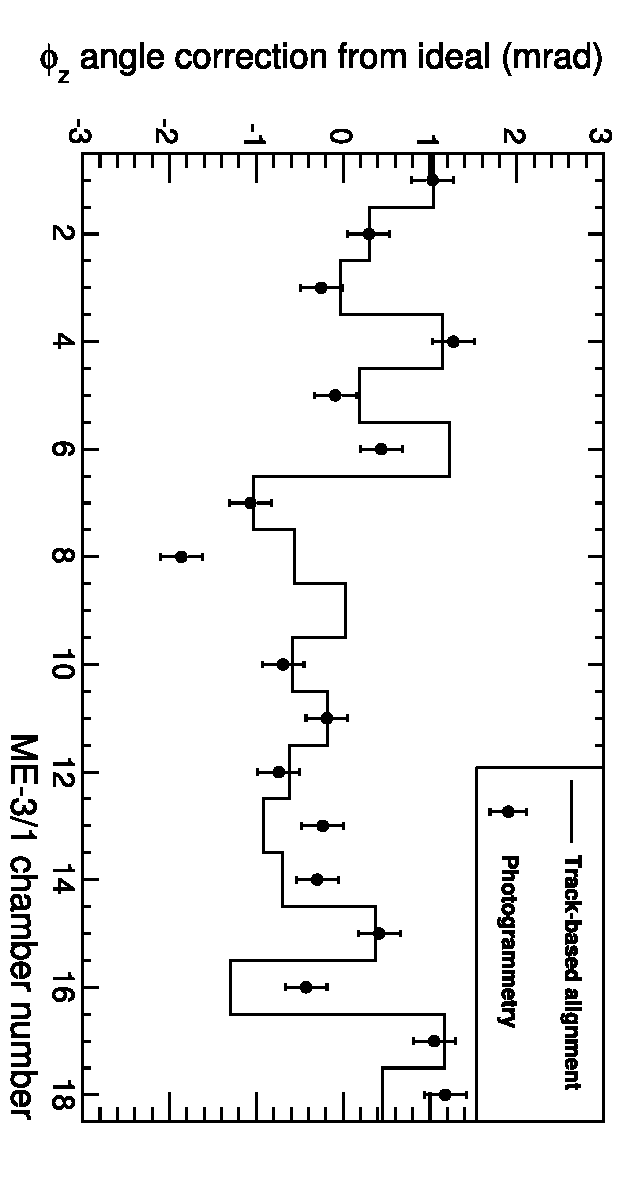
\includegraphics[height=0.48\linewidth, angle=90]{plots/csc_overlaps_alignment/compare_m31_phiz.pdf}
\end{minipage}
\end{center}
\caption{CSC alignment results from the Overlaps procedure and the 2008 LHC run, presented as a difference from ideal and compared with photogrammetry where possible. \label{fig:overlaps_data1}}
\end{figure}

\begin{figure}
\begin{center}
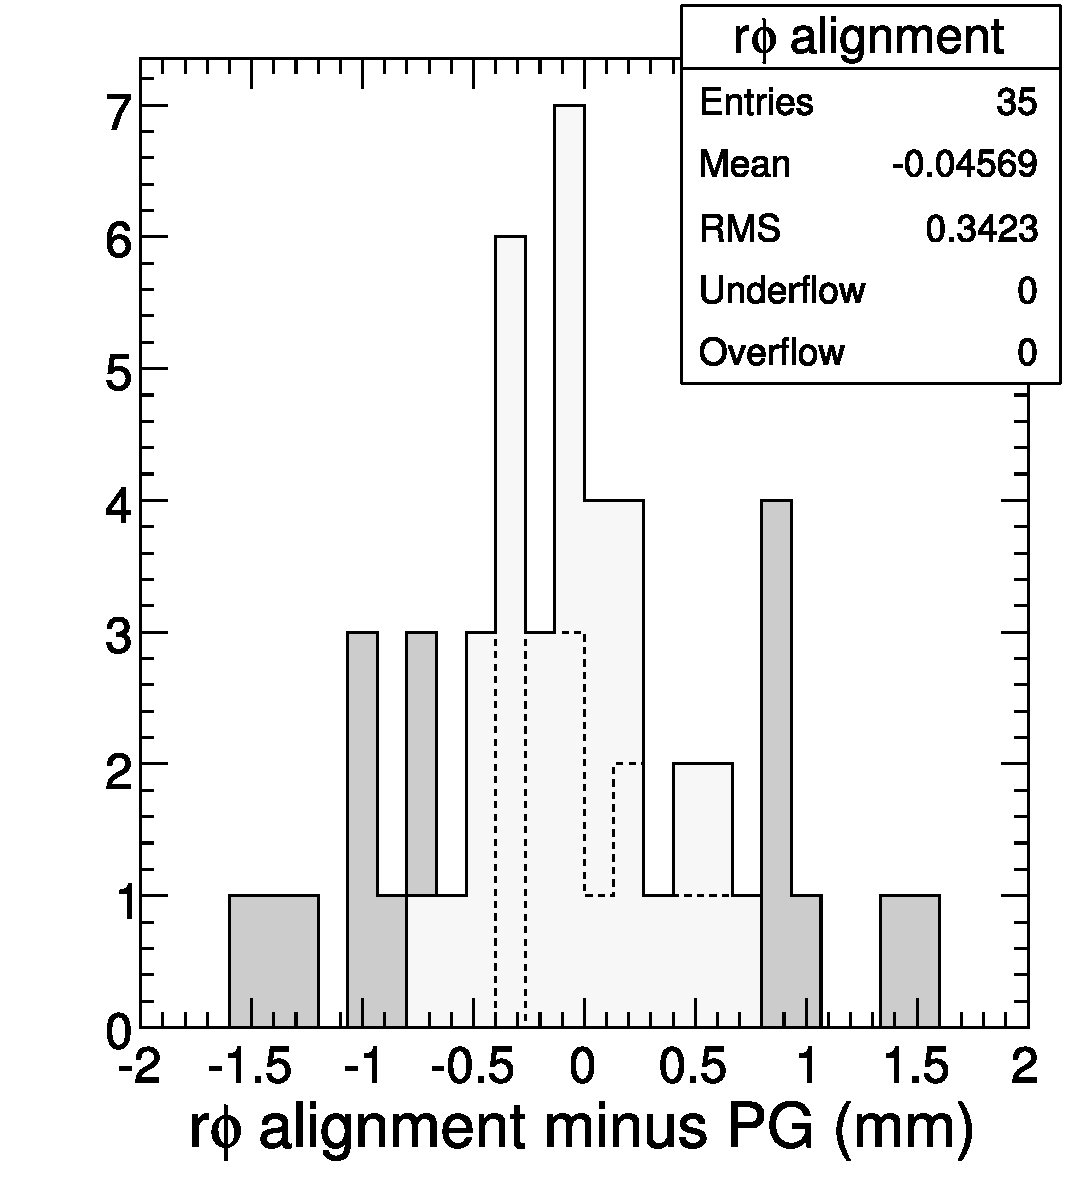
\includegraphics[width=0.35\linewidth]{plots/csc_overlaps_alignment/delta_translations_goodcolors.pdf} 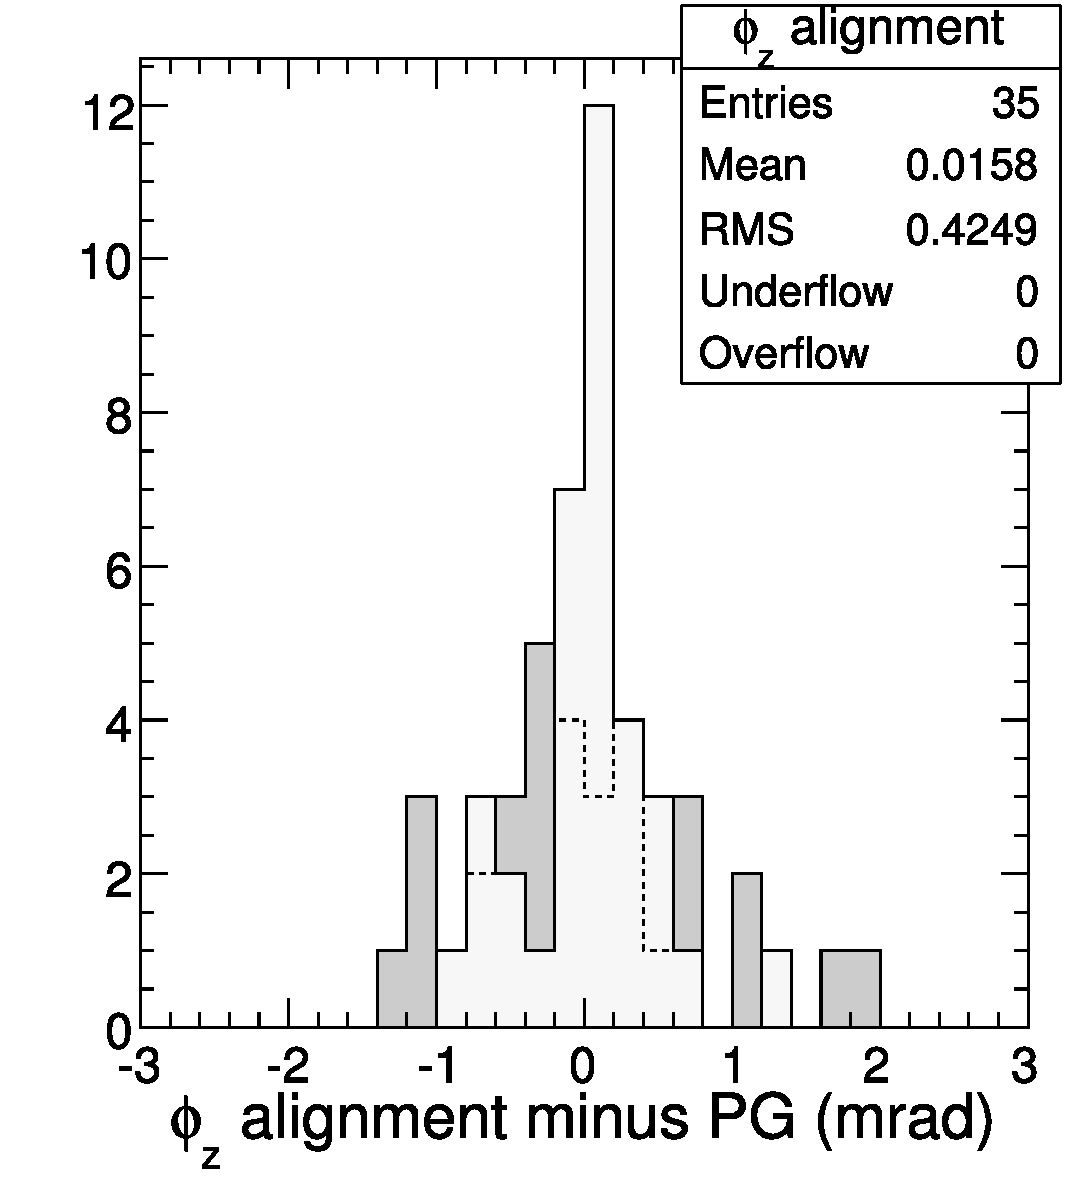
\includegraphics[width=0.35\linewidth]{plots/csc_overlaps_alignment/delta_rotations_goodcolors.pdf}
\end{center}
\caption{Chamber-by-chamber verification of the beam-halo alignment with photogrammetry.  The dark histogram is before alignment; the light histogram and statistics box are after alignment. \label{fig:overlaps_data2}}
\end{figure}

%% \begin{figure}
%% \begin{center}
%% 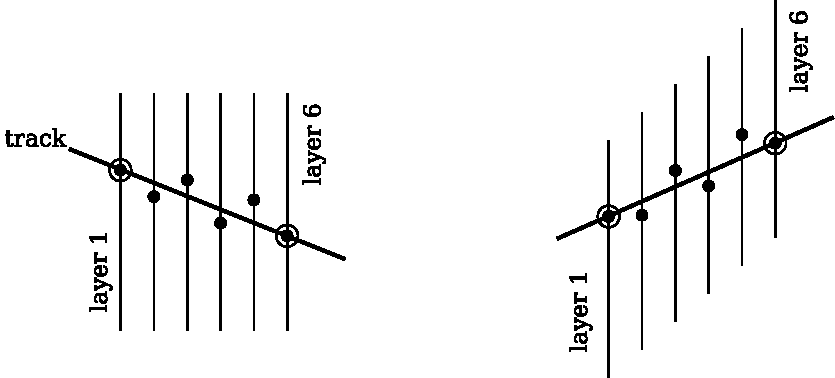
\includegraphics[width=0.75\linewidth]{plots/csc_overlaps_alignment/layer_alignment_skew.pdf}
%% \end{center}
%% \caption{Even when a track is constrained to two only layers, the positions of the other layers can only be determined up to a collective offset and a collective skew.  The two situations depicted here are indistinguishable. \label{fig:layer_alignment_skew}}
%% \end{figure}

%% \begin{figure}
%% \begin{center}
%% 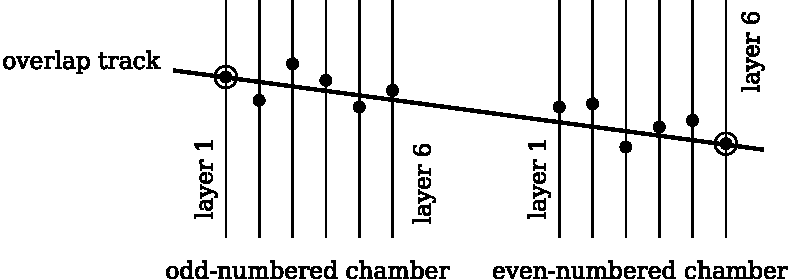
\includegraphics[width=0.75\linewidth]{plots/csc_overlaps_alignment/layer_alignment_noskew.pdf}
%% \end{center}
%% \caption{Method for aligning layers within chambers: constrain a linear track to the first and last layers in a two-chamber overlap, then align the remaining layers to that track. \label{fig:layer_alignment_noskew}}
%% \end{figure}

%% \begin{figure}
%% \begin{center}
%% 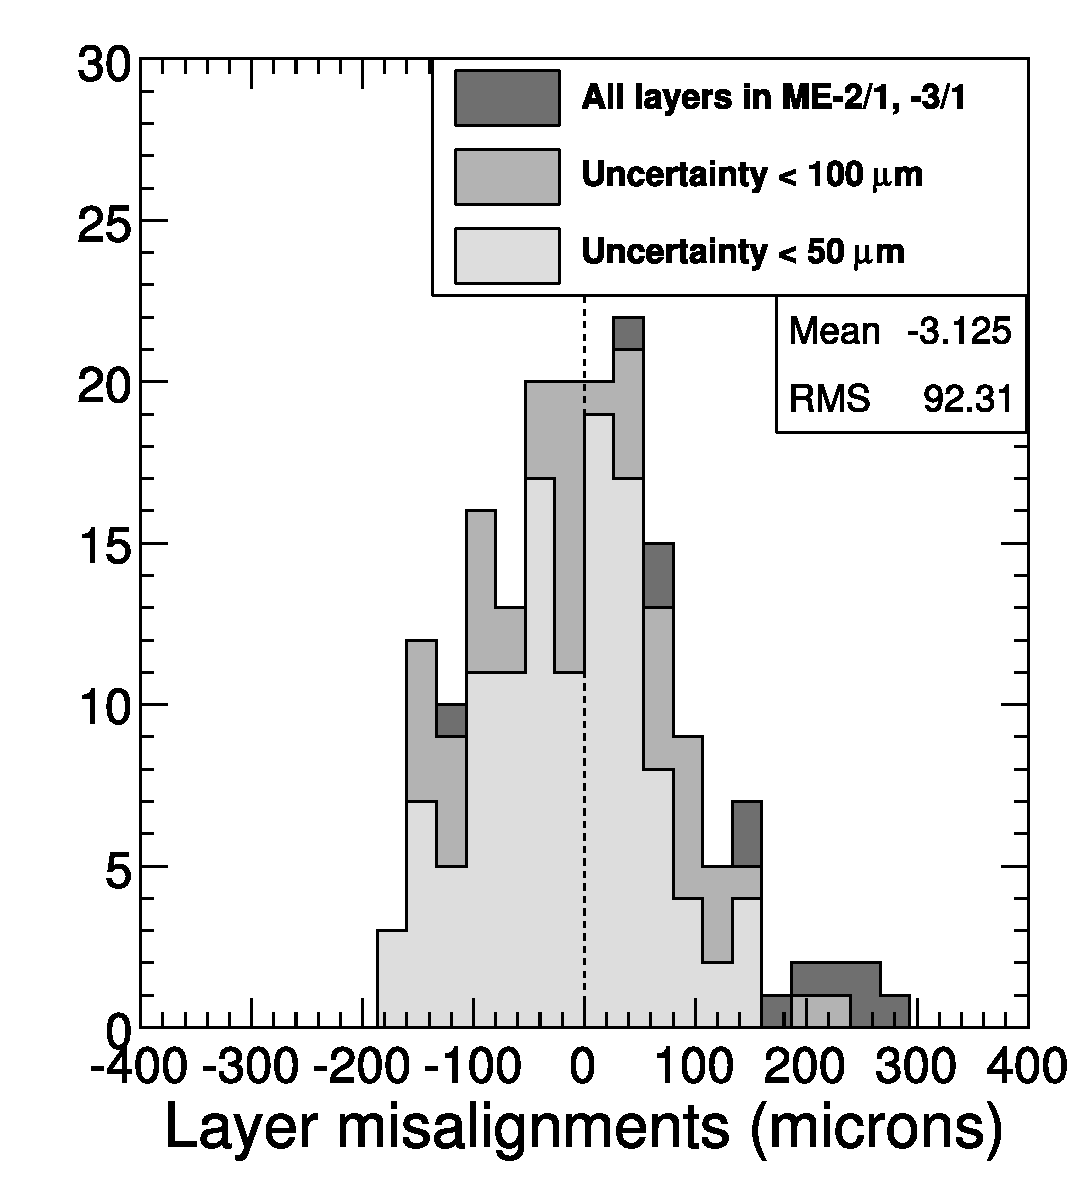
\includegraphics[width=0.5\linewidth]{plots/csc_overlaps_alignment/layer_hist.pdf}
%% \end{center}
%% \caption{Layer alignment results in ME$-$2/1 and $-$3/1, excluding layers fixed by definition. \label{fig:layer_hist}}
%% \end{figure}


%---------------------------------------------------------------------
\section{Global Muon Alignment}
\label{sec:global_muon_alignment}

Local muon alignment procedures arrange sets of chambers in
self-consistent coordinate systems, but cannot relate those
coordinates to the locations of other subsystems of CMS, particularly
the tracker.  In this section, we describe methods to
align muon chambers relative to the tracker, such that all
tracking volumes in CMS share one global system of coordinates.  Since
these global alignment methods are partly independent of the local alignments,
they can be used to cross-check each other.

Two algorithms, HIP (Hits and Impact Points) and Millepede, have been
developed to align muon chambers relative to the tracker.  Each is
described in its own section below, followed by studies in Monte Carlo
simulations, and then results of each with cosmic ray data.

\subsection{The HIP Algorithm}
\label{sec:hipalgo}
The basic idea of the HIP algorithm as it is applied to the muon
system is to fit alignables in a ``target'' tracking volume relative to a
well-aligned ``reference'' volume, usually the silicon tracker.  Muon
tracks are fitted using information from the reference volume only,
and chambers in the target are translated and rotated to minimize the
distance between muon hits and the impact points (intersections) of
tracks on the layer planes.  This differs from the conventional HIP
approach~\cite{ref:oldhip}, which iteratively aligns elements and fits tracks
in a single tracking volume.

Thick (20--60~cm) layers of iron are placed between each muon station
as a return yoke for the CMS solenoid.  In the iron, magnetic fields
are stronger than in the gas volume of the chambers, and probabilities
are higher that the muon's trajectory will 
scatter, making its direction less predictable between chambers than
within chambers.  To account for this correlation, we combine
residuals such that we obtain one independent measurement per chamber
per track.  This measurement has four components,
$\Delta x$, $\Delta y$, $\Delta \frac{dx}{dz}$, and $\Delta
\frac{dy}{dz}$, which are the differences between the propagated track's two-dimensional
location and entrance angle, respectively, with the pattern of hits in
the chamber.  We compute these four observables from a fit of the
residuals versus local $z$ to a straight line.
The reduced $\chi^2$ of the linear fit expresses
the quality of the measurement (independent of the distance between
the track and the hits), so we use $N_{\mbox{\scriptsize dof}}/\chi^2$
as a weight in the final alignment.  Station~4 DT chambers can only
measure one dimension, so they observe only $\Delta x$ and
$\Delta \frac{dx}{dz}$, and strip measurements in CSCs observe $\Delta
r\phi$ and $\Delta d(r\phi)/dz$.

The measurements described above are influenced by four categories of effects:
\begin{itemize}
\item misalignment of the target chamber (geometric residuals),
\item statistical uncertainty in the track fit,
\item propagation errors from large-angle scattering (distributes
residuals according to a power law) and the result of many small-angle
scattering events (Gaussian ``multiple scattering''),
\item biases in the track source or chamber itself.
\end{itemize}
Our goal is to identify errors of the first category, though the first
three are convoluted together in a statistical distribution, and the
fourth can only be diagnosed by an independent method (such as local
alignment techniques described in the previous sections).

Assuming that we can isolate geometric residuals ${\Delta
  x}^{\mbox{\scriptsize geom}}$, ${\Delta y}^{\mbox{\scriptsize
    geom}}$, ${\Delta \frac{dx}{dz}}^{\mbox{\scriptsize geom}}$, and
${\Delta \frac{dy}{dz}}^{\mbox{\scriptsize geom}}$, the alignment
corrections $\delta_x$, $\delta_y$, $\delta_z$, $\delta_{\phi_x}$,
$\delta_{\phi_y}$, and $\delta_{\phi_z}$ can be computed by solving
the equation:
\begin{equation}
\renewcommand{\arraystretch}{2.5}
\left(\begin{array}{c}
{\Delta x}^{\mbox{\scriptsize geom}} \\
{\Delta y}^{\mbox{\scriptsize geom}} \\
{\Delta \dfrac{dx}{dz}}^{\mbox{\scriptsize geom}} \\
{\Delta \dfrac{dy}{dz}}^{\mbox{\scriptsize geom}} \\
\end{array}\right)
=
{\renewcommand{\arraystretch}{2.5}
\left(\begin{array}{c c c c c c}
1 & 0 & -\dfrac{dx}{dz} & -y \dfrac{dx}{dz} & x \dfrac{dx}{dz} & -y \\
0 & 1 & -\dfrac{dy}{dz} & -y \dfrac{dy}{dz} & x \dfrac{dy}{dz} & x \\
0 & 0 & 0 & -\dfrac{dx}{dz} \dfrac{dy}{dz} & 1 + \left(\dfrac{dx}{dz}\right)^2 & -\dfrac{dy}{dz} \\
0 & 0 & 0 & -1 - \left(\dfrac{dy}{dz}\right)^2 & \dfrac{dx}{dz}\dfrac{dy}{dz} & \dfrac{dx}{dz}
\end{array}\right)}
\renewcommand{\arraystretch}{1.7}
\left(\begin{array}{c}
\delta_x \\
\delta_y \\
\delta_z \\
\delta_{\phi_x} \\
\delta_{\phi_y} \\
\delta_{\phi_z}
\end{array}\right) \mbox{.}
\label{eqn:dtmatrix}
\end{equation}
(The above matrix is an extension of Equation~17 in~\cite{ref:oldhip}).
For CSCs, the curvilinear residuals ${\Delta r\phi}^{\mbox{\scriptsize
geom}}$ and ${\Delta
d(r\phi)/dz}^{\mbox{\scriptsize geom}}$ introduce corrections suppressed by $r$, the radial
distance to the beamline:
\begin{equation}
\renewcommand{\arraystretch}{3}
\left(\begin{array}{c}
{\Delta r\phi}^{\mbox{\scriptsize geom}} \\
{\Delta \dfrac{dr\phi}{dz}}^{\mbox{\scriptsize geom}} \\
\end{array}\right)
=
{\renewcommand{\arraystretch}{3}
\left(\begin{array}{c c c c c c}
1 & \left[ -\dfrac{x}{r} + 3\left(\dfrac{x}{r}\right)^3 \right] & -\dfrac{dx}{dz}  & -y \dfrac{dx}{dz} & x \dfrac{dx}{dz} & -y \\
0 & -\dfrac{dx}{dz} \left(\dfrac{1}{2r}\right) & 0 & \left[ \dfrac{x}{r} - \dfrac{dx}{dz}\dfrac{dy}{dz} \right] & 1 + \left(\dfrac{dx}{dz}\right)^2 & -\dfrac{dy}{dz}
\end{array}\right)}
\renewcommand{\arraystretch}{1}
\left(\begin{array}{c}
\delta_x \\
\delta_y \\
\delta_z \\
\delta_{\phi_x} \\
\delta_{\phi_y} \\
\delta_{\phi_z}
\end{array}\right) \mbox{.}
\label{eqn:cscmatrix}
\end{equation}

To extract geometric residuals from the measurements, we construct an
ansatz describing all effects and fit it to the data.  Each of the
four observables is represented by a convolution of a Gaussian and a
Lorentzian (to model the power-law scattering tails),
\begin{equation}
f(t; \, t_0, \, \sigma, \, \gamma) = \int_{-\infty}^\infty
\frac{1}{\pi}\frac{\gamma}{(t - s - t_0)^2 + (\gamma)^2} \times 
\frac{1}{\sqrt{2\pi} \sigma} \exp\left(\frac{-s^2}{2
  \sigma^2}\right) \, ds \mbox{.}
\label{eqn:fitfunction}
\end{equation}
Position residuals are correlated with their corresponding angle
residuals because any error in the propagated track's direction
upstream of the chamber causes errors in its position to grow.
Therefore, a 2-D distribution of $\Delta x$ and $\Delta \frac{dx}{dz}$
is skewed by a parameter $\alpha_{\Delta x}$.  A fit function for all
four residuals, $F$, is the product of four instances of $f$:
\begin{multline}
F\bigg(\Delta x, \Delta y, \Delta \tfrac{dx}{dz}, \Delta \tfrac{dy}{dz}; \\
{\Delta x}_0, {\Delta y}_0, {\Delta \frac{dx}{dz}}_0, {\Delta \frac{dy}{dz}}_0,
\sigma_{\Delta x}, \sigma_{\Delta y}, \sigma_{\Delta \tfrac{dx}{dz}}, \sigma_{\Delta \tfrac{dy}{dz}}, 
\gamma_{\Delta x}, \gamma_{\Delta y}, \gamma_{\Delta \tfrac{dx}{dz}}, \gamma_{\Delta \tfrac{dy}{dz}}, 
\alpha_{\Delta x}, \alpha_{\Delta y}) = \\
f\bigg(\Delta x; \, \big({\Delta x}_0 + \alpha_{\Delta x} \Delta \tfrac{dx}{dz}\big), \, \sigma_{\Delta x}, \, \gamma_{\Delta x}\bigg) \, \times \,
f\bigg(\Delta \tfrac{dx}{dz}; \, {\Delta \tfrac{dx}{dz}}_0, \, \sigma_{\Delta \tfrac{dx}{dz}}, \, \gamma_{\Delta \tfrac{dx}{dz}}\bigg) \\
f\bigg(\Delta y; \, \big({\Delta y}_0 + \alpha_{\Delta y} \Delta \tfrac{dy}{dz}\big), \, \sigma_{\Delta y}, \, \gamma_{\Delta y}\bigg) \, \times \,
f\bigg(\Delta \tfrac{dy}{dz}; \, {\Delta \tfrac{dy}{dz}}_0, \, \sigma_{\Delta \tfrac{dy}{dz}}, \, \gamma_{\Delta \tfrac{dy}{dz}}\bigg)
\end{multline}

The peak of this distribution, $({\Delta x}_0, \, {\Delta y}_0,
\, {\Delta \frac{dx}{dz}}_0, \, {\Delta\frac{dy}{dz}}_0)$, can be
identified as the geometric residuals on the left-hand-side of
Equation~\ref{eqn:dtmatrix} because the observed distribution of
residuals is further convoluted by misalignment.  The effect of
misalignment is not random; its distribution would be described by a
system of delta distributions that simply replace $({\Delta x}_0, \, {\Delta y}_0,
\, {\Delta \frac{dx}{dz}}_0, \, {\Delta\frac{dy}{dz}}_0)$ with 
$({\Delta x}^{\mbox{\scriptsize geom}},\mbox{ }{\Delta
y}^{\mbox{\scriptsize geom}},\mbox{
}{\Delta \frac{dx}{dz}}^{\mbox{\scriptsize geom}},\mbox{
}{\Delta \frac{dy}{dz}}^{\mbox{\scriptsize geom}})$ and introduce a
dependence on the track impact positions $x$, $y$ and entrance angles
$\tfrac{dx}{dz}$, $\tfrac{dy}{dz}$.  The final fit function has 16
parameters and 8 dimensions for DT stations 1--3, 11 parameters and 6
dimensions for CSCs, and 10 parameters, 6 dimensions for DT station~4
(no access to $\delta_y$).  The most relevant projections of an
example fit are shown in Figure~\ref{fig:examplefit}.  The fit is
performed by MINUIT~\cite{ref:minuit} with an unbinned maximum
likelihood method, using the weights described above.

\begin{figure}
\begin{center}
\subfigure[Projection of residuals onto impact point and entrance angle, before alignment.]{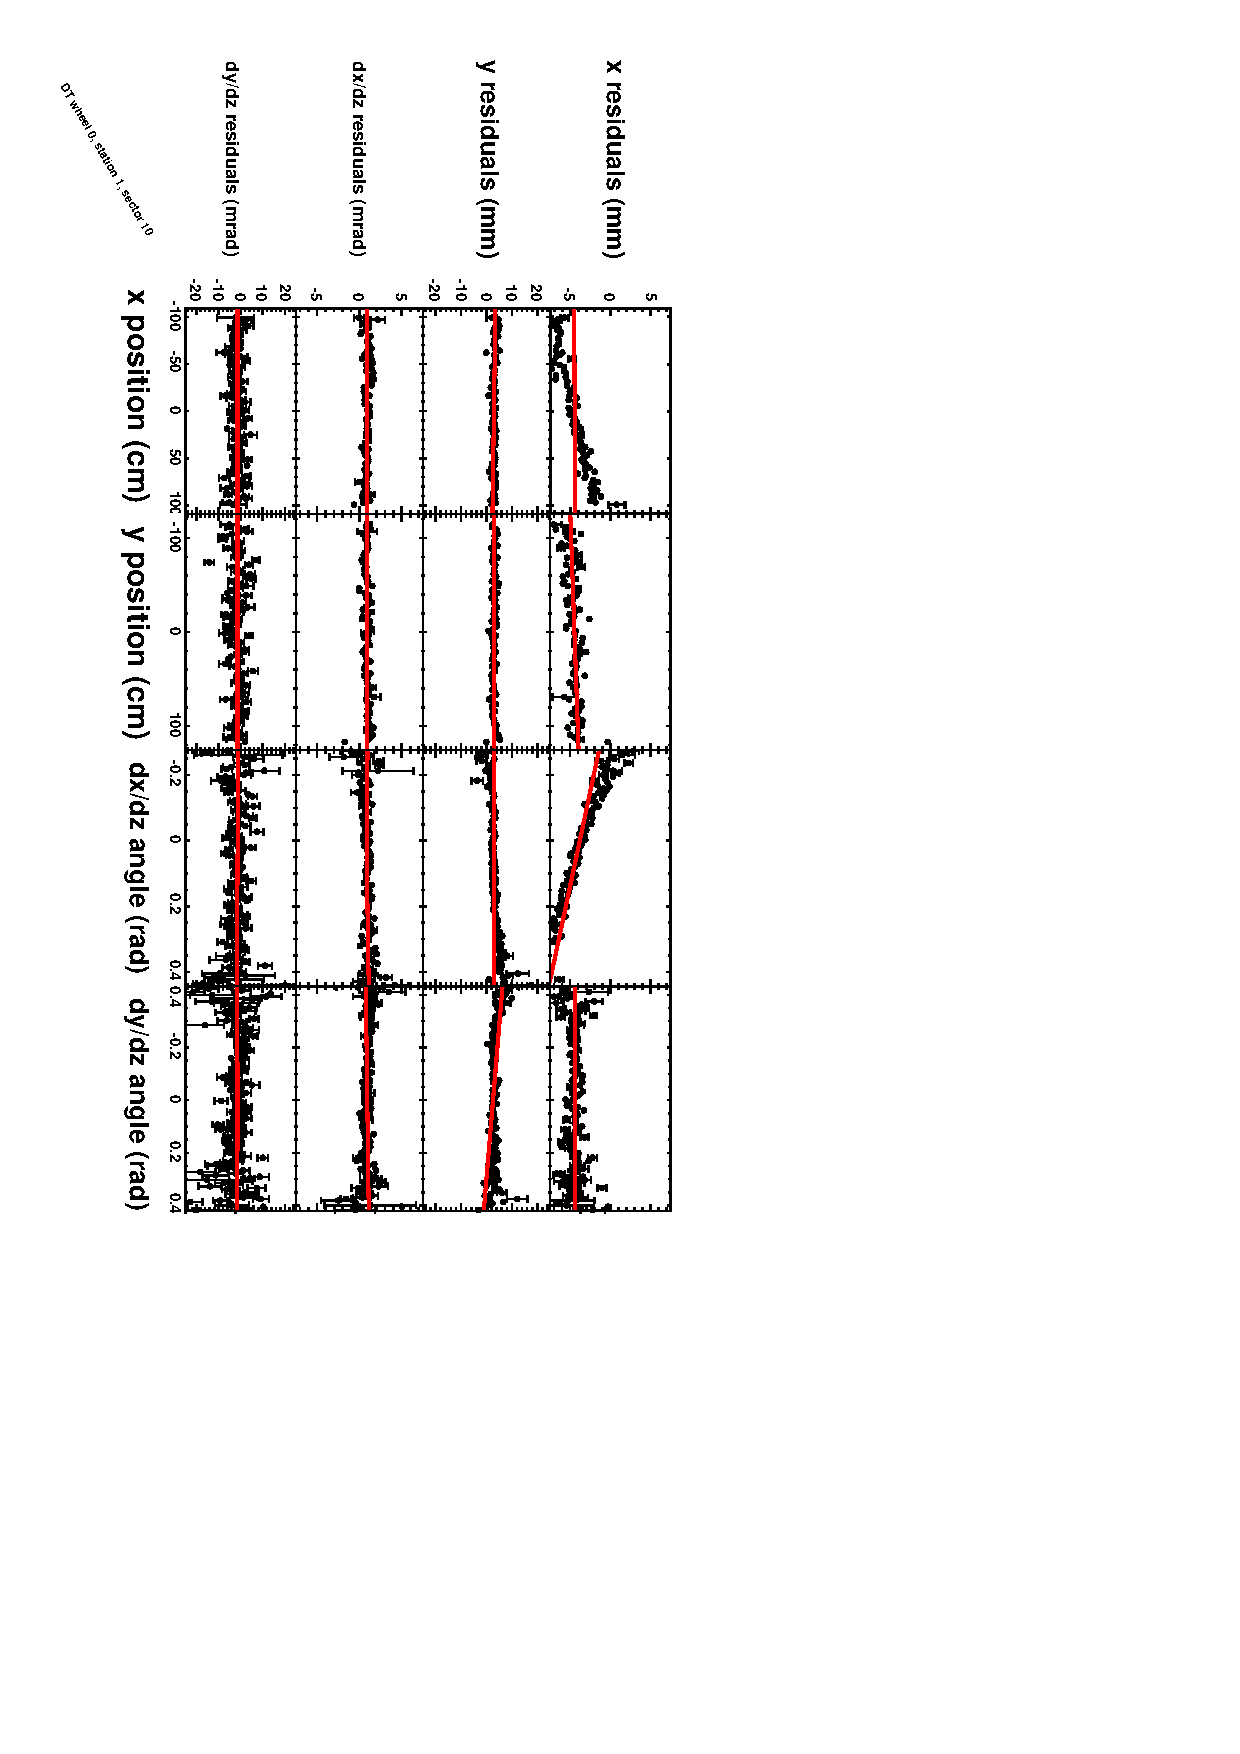
\includegraphics[height=0.75\linewidth, angle=90]{plots/gma_hip_algorithm/exampleData_wh0st1sec10_polybefore.pdf}}

\subfigure[Projection of residuals onto impact point and entrance angle, after alignment. \label{fig:examplefitb}]{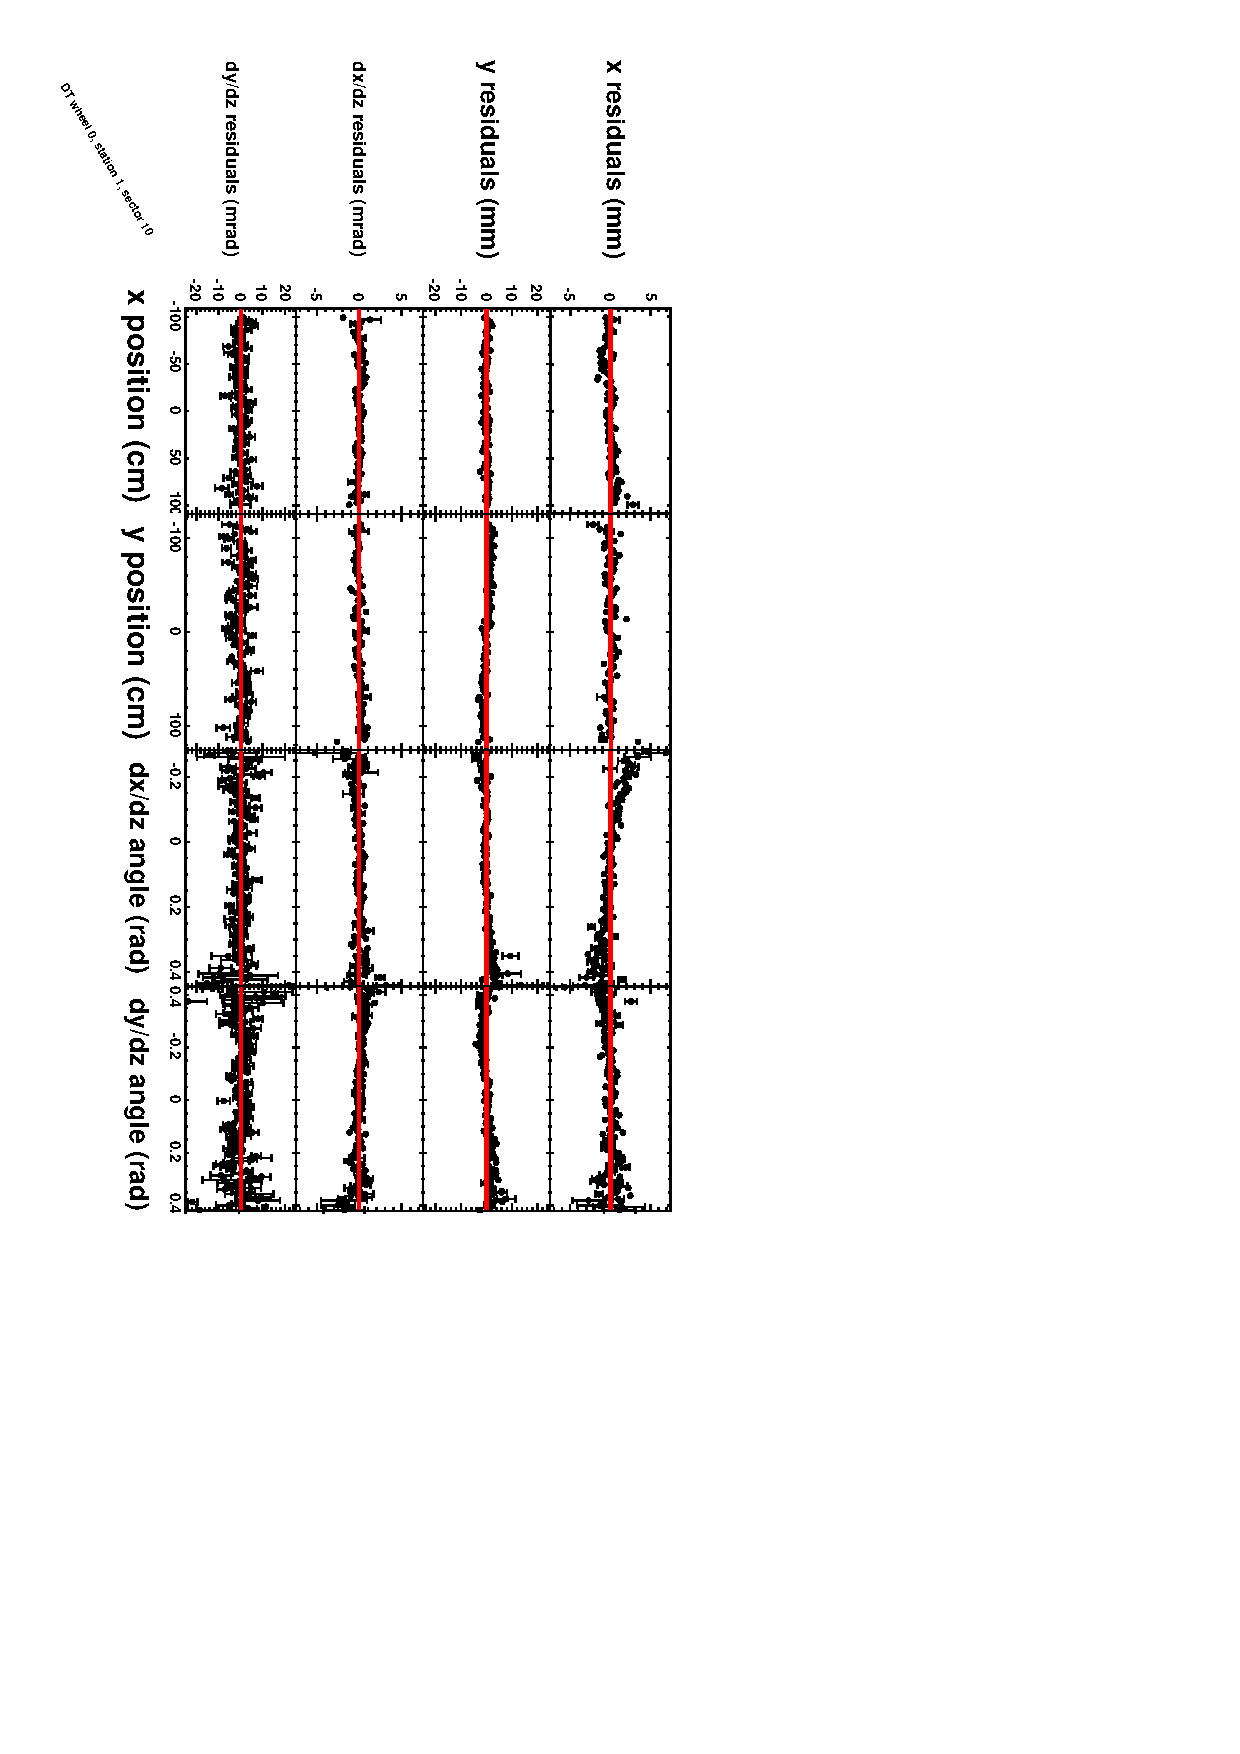
\includegraphics[height=0.75\linewidth, angle=90]{plots/gma_hip_algorithm/exampleData_wh0st1sec10_polyafter.pdf}}

\subfigure[Projection of residuals and their correlations, after alignment.]{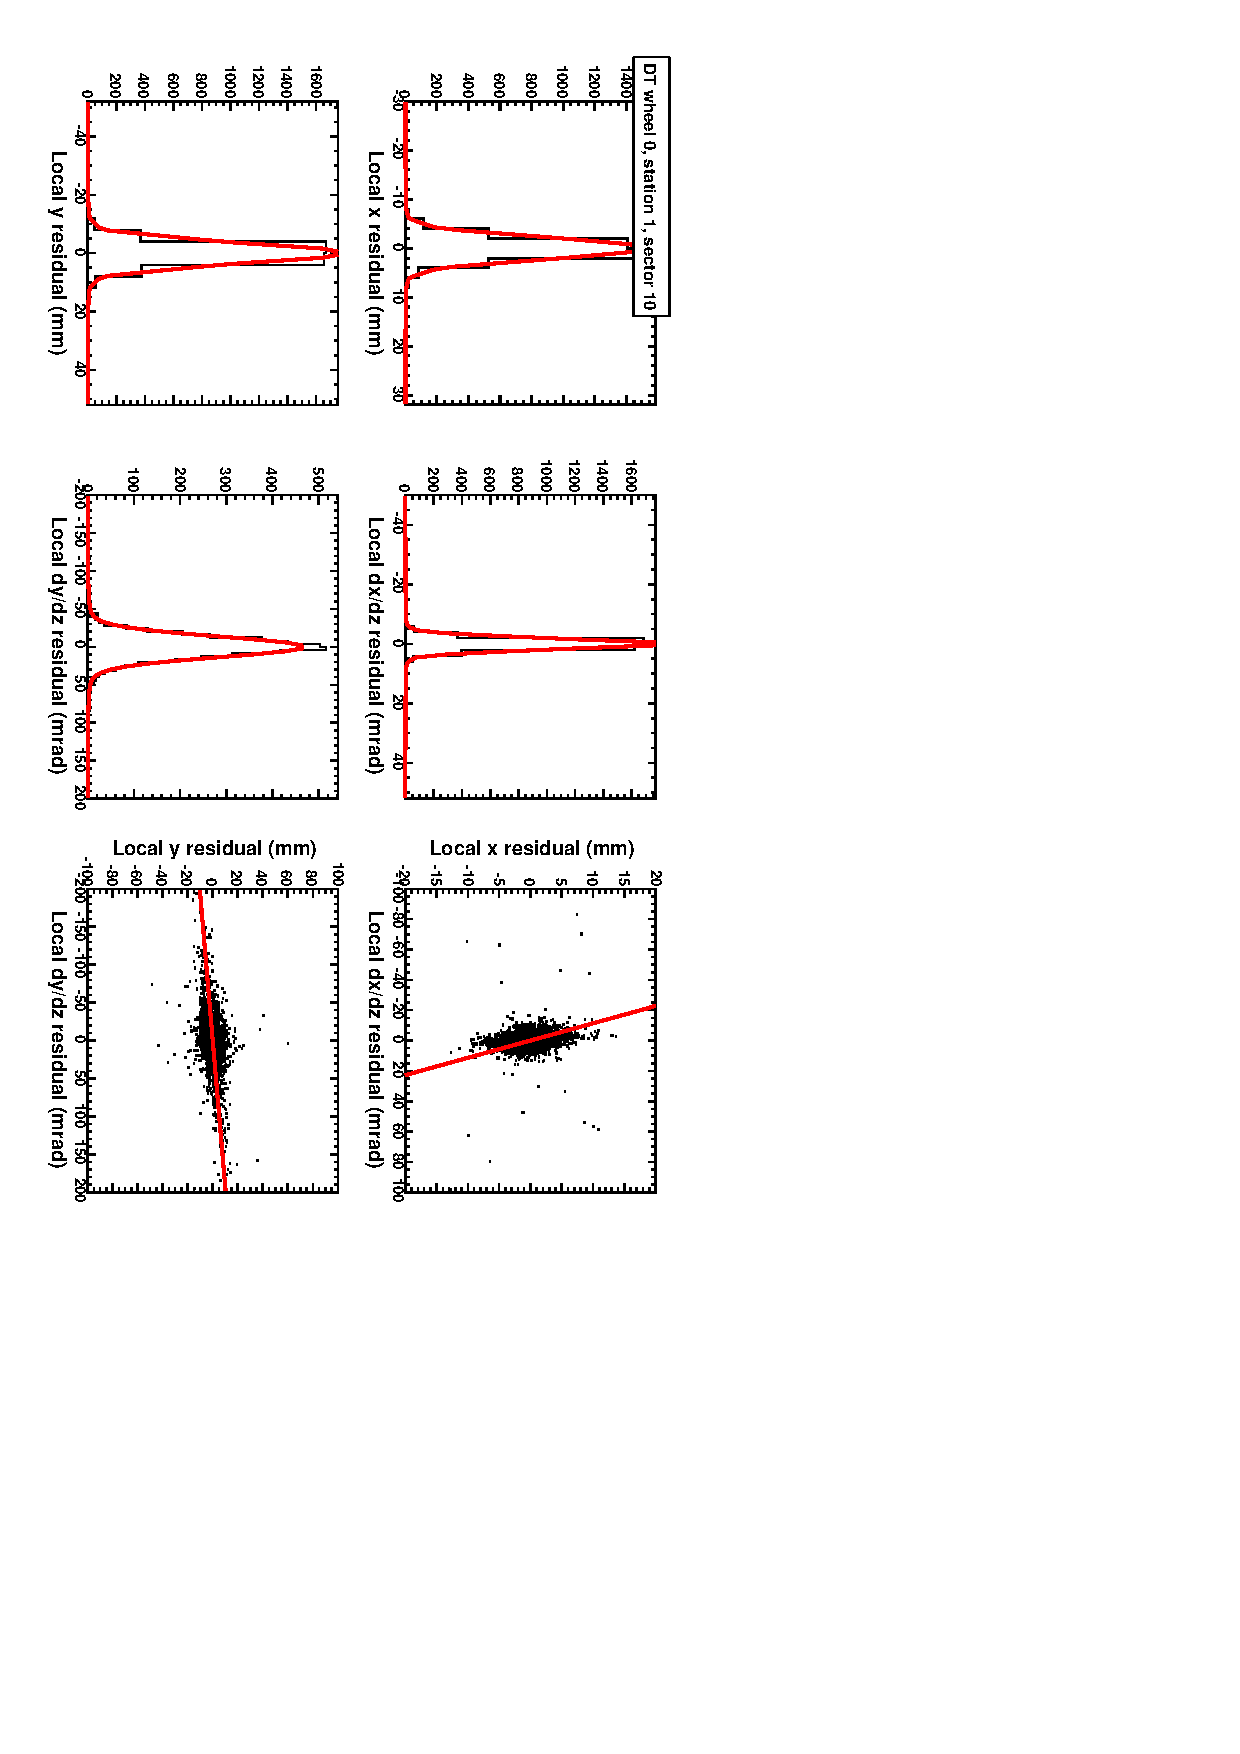
\includegraphics[height=0.75\linewidth, angle=90]{plots/gma_hip_algorithm/exampleData_wh0st1sec10_bellafter.pdf}}
\end{center}

\caption{An example fit to cosmic ray data (DT wheel~0, station~1, sector~10) from the HIP algorithm.  The red lines are projections of the fit result. \label{fig:examplefit}}
\end{figure}

If the magnetic field or material maps are not perfectly represented
in track propagation, residuals will be biased as an antisymmetric
function of track curvature, $q/p_T$.  To correct for any such errors,
we split the sample into two bins, one for each charge $q$, and
perform the alignment separately in each bin.  Muons and antimuons
have the same spectral distribution in cosmic rays (though not the
same flux), so a simple average of the $q<0$ and $q>0$ results cancels the
antisymmetric bias in all alignment corrections except $\delta_z$.
The difference of the two bins is maximally sensitive to the bias and
can be used to measure it.

Repeated applications of the procedure converge quickly to an optimal
solution.  Significant corrections are only observed in the first and
second iterations (in data and simulation), so we always perform three
iterations.
  

\subsection{The MilliPede Algorithm}
The Millepede-based algorithm implemented for global alignment is a
particular case of the most general Millepede algorithm already
referred to in section~\ref{sec:localdt}.  In this case, the ability
to fit tracks and alignment parameters together is parameterized, such
that the algorithm can either let them both float freely (full
Millepede), or align chambers to a fixed set of tracks (alignment to
reference).

To align chambers in CRAFT, the algorithm was tuned to use a fixed set
of tracks from the tracker.  These tracks were propagated into the
muon system, and unbiased residuals distributions were minimized by
aligning chambers.  In the language of section~\ref{sec:localdt}, the
matrices $B_j \to 0$ and $\delta \vec{p}_j$ are no longer parameters
in the fit.  This also decorrelates alignment parameters in different
chambers, greatly simplifying the alignment.

As described
in section~\ref{sec:hipalgo}, the scattering processes that take place in the iron yoke between chambers
deflect muons in a correlated pattern for all the hits in a same chamber. To account
for this correlation, single layer hits and the track intersections associated to them
are combined in a linear fit producing four observables for each chamber: the position
residuals $\Delta x$, $\Delta y$ and the direction
residuals $\Delta \frac{dx}{dz}$ and $\Delta \frac{dy}{dz}$.
Just as in the HIP case, these residuals are related to the 6 alignment parameters $\delta_x$,
$\delta_y$, $\delta_z$, $\phi_x$, $\phi_y$ and $\phi_z$, by Equation~\ref{eqn:dtmatrix}.

The form of the $\chi^2$ associated with the general Millepede algorithm was shown in Equation~\ref{eqn:chi2millepede}.
In this implementation of the algorithm, $\chi^2$ has the form     
\begin{equation}
{\chi^2}^{\mbox{\scriptsize \, track-based}} = \sum_j \left(\Delta \vec{x} - A \cdot \vec{\delta} \right)^T \, \left({\sigma_{\mbox{\scriptsize resid}_{\mbox{\scriptsize $i$}}}}^2\right)^{-1} \, \left(\Delta \vec{x} - A \cdot \vec{\delta} \right)
\label{eqn:globalmpchi2}
\end{equation}
where the $\Delta \vec{x}$ is a 4-component vector, and
$A$ is the matrix which relates the residuals with the alignment parameters. The 
$\left({\sigma_{\mbox{\scriptsize resid}_{\mbox{\scriptsize $i$}}}}^2\right)^{-1}$ matrix
is the inverse of the covariance calculated from the linear fit estimation of the segments. It
includes correlations between positions and directions in both projections.

To avoid the influence of the tails of the residuals distributions, a
filtering operation is performed.  This is especially important
because the tails of the distributions may not be perfectly symmetric.
To set cut boundaries for the residuals on each chamber, the peak is
fitted to a Lorentz function and residuals are required to be within
the full width at half maximum (between $x_0 - \Gamma/2$ and $x_0
+ \Gamma/2$ where $x_0$ and $\Gamma$ are the peak and full-width at
half maximum, respectively).  In a one-dimensional application, this
alignment fit would correspond to a truncated mean.
  

\subsection{Monte Carlo Study and Discussion of Systematic Errors}
We tested the algorithms with three Monte Carlo simulations: a
geometry-only toy simulation to observe the geometric effects
independent of detector effects, a full Pythia and GEANT-based
$pp \to \mu + X$ collisions sample, and a full GEANT-based cosmic ray
sample.  The sizes of the simulated event samples are all large enough
for the alignment results to be systematics-limited, and in the
GEANT-based simulations, all detector effects were modelled except
tracker misalignment, magnetic field errors, and internal muon chamber
misalignment.  This demonstrates the alignment reach of the algorithms
themselves, apart from any possible deficiencies in the input
tracks, propagation model, and chamber geometry.

The initial muon system misalignment used in these studies was a
Gaussian smearing of chamber positions with a 2~mm standard deviation in $\delta_x$,
4~mm in $\delta_y$ and $\delta_z$, and 2~mrad in the three angles.  We
then applied each procedure to the simulated events in exactly the
same way we do to data.  Different initial misalignments yield the
same results.

Figure~\ref{fig:hip_MC} shows differences between aligned positions of
each parameter and their true positions for the two algorithms in
simulated cosmic rays.  Interpreting the RMS of these distributions as
the alignment accuracy, the $\delta_x$ accuracy is 200~$\mu$m for HIP,
500~$\mu$m for Millepede, close to the intrinsic hit uncertainty of
100--300~$\mu$m.  Statistical uncertainties returned by the fits are a
factor of 3--4 times smaller than the observed accuracy, so this
represents the systematic limit of the algorithms as they are
currently defined.

\begin{figure}
\subfigure[HIP aligned-minus-true positions before (purple) and after (yellow) alignment.]{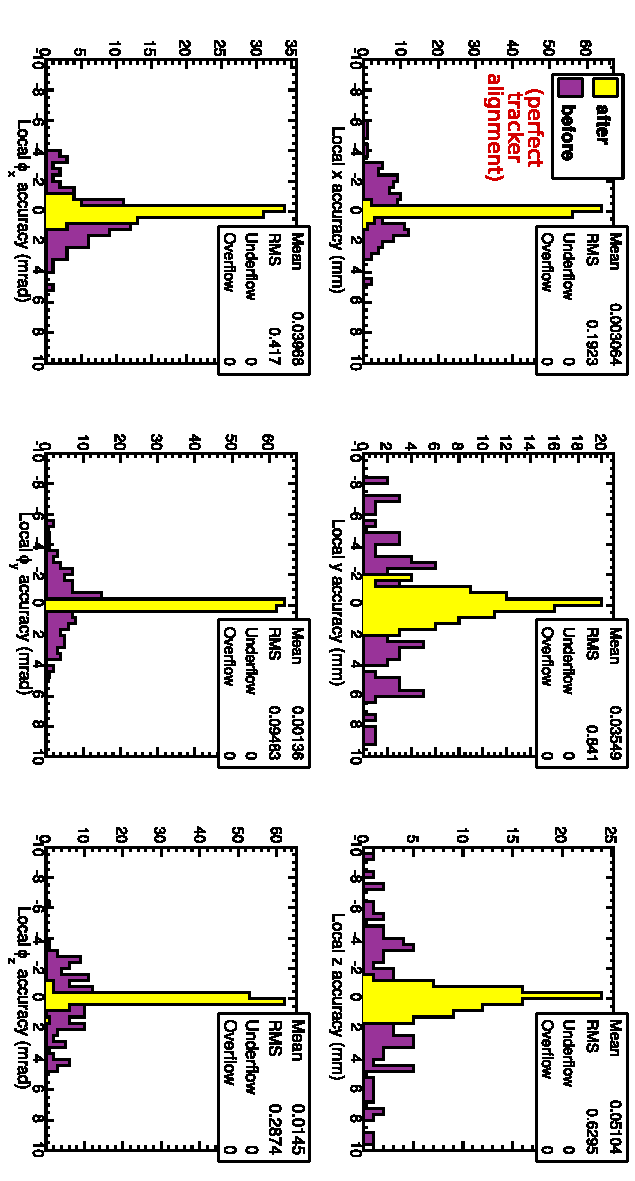
\includegraphics[height=\linewidth, angle=90]{plots/mc_and_syst_studies/hip_MC.pdf}}

\subfigure[Millepede aligned-minus-true positions before (purple) and after (yellow) alignment.]{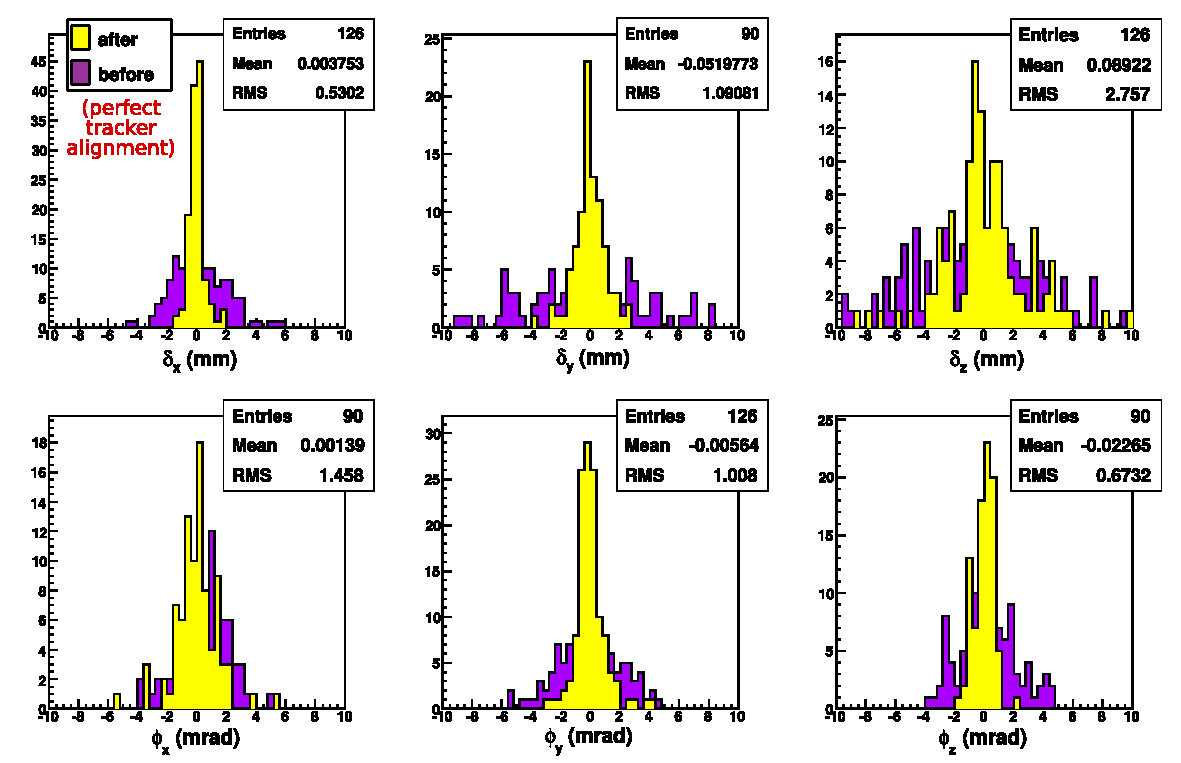
\includegraphics[width=\linewidth]{plots/mc_and_syst_studies/Millipede_MC_RandomScenario.pdf}}

\caption{Alignment with simulated cosmic rays using (a) HIP and (b) Millepede.  Each
  entry in the histograms is the difference between the aligned and
  true values of alignment parameters for one DT
  chamber.  (Only aligned parameters are shown: $\delta_x$,
  $\delta_{\phi_y}$ and $\delta_{\phi_z}$ for station~4 and all 6
  parameters for stations 1--3.) \label{fig:hip_MC}}
\end{figure}

There are four classes of systematic error in these procedures:
(1) simplifying assumptions about the residuals distributions,
(2) biases in the input set of tracks,
(3) errors in the propagation of tracks through the muon system, and
(4) internal misalignments in the chambers.
The exercise described above addresses the first of these, in that the
Monte Carlo simulation represents a complete model of the detector
response~\cite{ref:dtlocalreco}, while the alignment algorithms both
include simplifications, optimized for finding the underlying
misalignment.  The Millepede performance is expected to improve by
including a more realistic description of the covariance
${\sigma_{\mbox{\scriptsize resid}_{\mbox{\scriptsize
$i$}}}}^2$ (Equation~\ref{eqn:globalmpchi2}) and a better
treatment of the tails of the residuals distribution.

The question of whether input tracks were biased (2) can be addressed in several ways.
One is to compare local alignment information with global information,
as only the latter would be affected by a biased global tracks.  This
cross-check was performed and is presented in the next section.
Another test uses the fact that muon chambers are large rigid bodies:
residuals inside the chambers must be linear with respect to $x$, $y$,
$\tfrac{dx}{dz}$, and $\tfrac{dy}{dz}$, but can be discontinuous at
the thresholds between chambers.  Discontinuities such as these can
only be caused by misalignments, as the input track distribution is
unlikely to have features at these points.  Small input track biases, below
the limit of what could be observed by these methods, would distort
the aligned positions of chambers, but in such a way that optimizes
the tracking resolution of the selected input tracks.

As tracks propagate into the muon system (3), they may be systematically
distorted by potential errors in the magnetic field map and material
budget, in a way which reverses sign with muon charge.  Application of
the procedure described in~\ref{sec:hipalgo} to correct for this
effect resulted in negligible alignment differences (100~$\mu$m,
200~$\mu$m, and 350~$\mu$m
in $\delta_x$, $\delta_y$, and $\delta_z$ and 0.1~mrad in the angles).

Finally, internal misalignments (4) change the effective center of the
chamber, making the global alignment results harder to interpret in
comparison with physical landmarks (such as the hardware alignment
system), but no less valid for track reconstruction.



\subsection{Global Alignment Results and Cross-Checks}
Both the HIP and Millepede algorithms were applied to align a subset
of barrel chambers during the CRAFT
data-taking run.  Wheels $-$1, 0, and $+$1 were aligned, with the
exception of sectors 1 and 7 (extreme horizontal sides of the
detector) using the barrel section of the tracker as the track
reference.  The alignment was restricted to this central subset of the
barrel chambers because they were the only ones sufficiently
illuminated by the primarily vertical distribution of cosmic rays.  We
also restricted the input to high-quality $100 < p_T < 200$~GeV tracks
with at least 15 tracker hits and a tracker reduced $\chi^2 < 10$.
Loosening these cuts does not make significantly more chambers
available for alignment.  The dataset included all runs marked as acceptable for
physics in the CMS run registry, with a magnetic field of 3.8~T.  The
CRAFT period included several on-off cycles of the magnetic field,
which were shown to result in reproducible alignments with the
hardware system~\cite{ref:hardware_alignment} and tracks (within
statistical precision).

In addition to the chambers explicitly excluded from alignment due to
poor statistics, two chambers next to sectors 1 and 7 (in wheel,
station, sector ($-$1, 2, 8) and ($+$1, 3, 8)) had no tracks passing
the cuts and two more (($-$1, 1, 12) and ($+$1, 2, 2)) failed to
converge in HIP, owing to the extreme azimuthal asymmetry of cosmic
rays underground.

We checked our alignment results in four ways: we verified (1) that
the algorithms optimized their intended expressions, (2) that they
agree with one another, (3) that the new global chamber positions yield the same or
better agreement with local measurements, and (4) that the new
alignment yields better momentum resolution for tracks.

The simplest way to test the internal consistency of the algorithm (1)
is to run the alignment algorithm a second time on the same dataset
and verify that the second alignment corrections are always zero.  As
a sanity check, we also verified that the raw residuals distributions
are centered at zero with very high precision.  An example of this was
shown in Figure~\ref{fig:examplefit}.

To demonstrate that the two algorithms agree with each other (2), we
present corrections computed by each algorithm in a scatter
plot~\ref{fig:sidebyside}.  Though the corrections were on the order
of 0.5--3~mm/mrad, the two algorithms agree with each other within
expectations from the Monte Carlo study (Figure~\ref{fig:hip_MC}).  The
two parameters in which no correlation is observed between the
algorithms are $\delta_z$ and $\delta_{\phi_z}$, which are the most
likely to be affected by the treatment of tails in residuals
distributions.  The distributions of $\delta_y$ and $\delta_{\phi_x}$
have tall peaks at zero: these parameters cannot be aligned in
station~4, because station~4 chambers do not measure $\Delta y$
residuals.

\begin{figure}
\begin{center}
%% 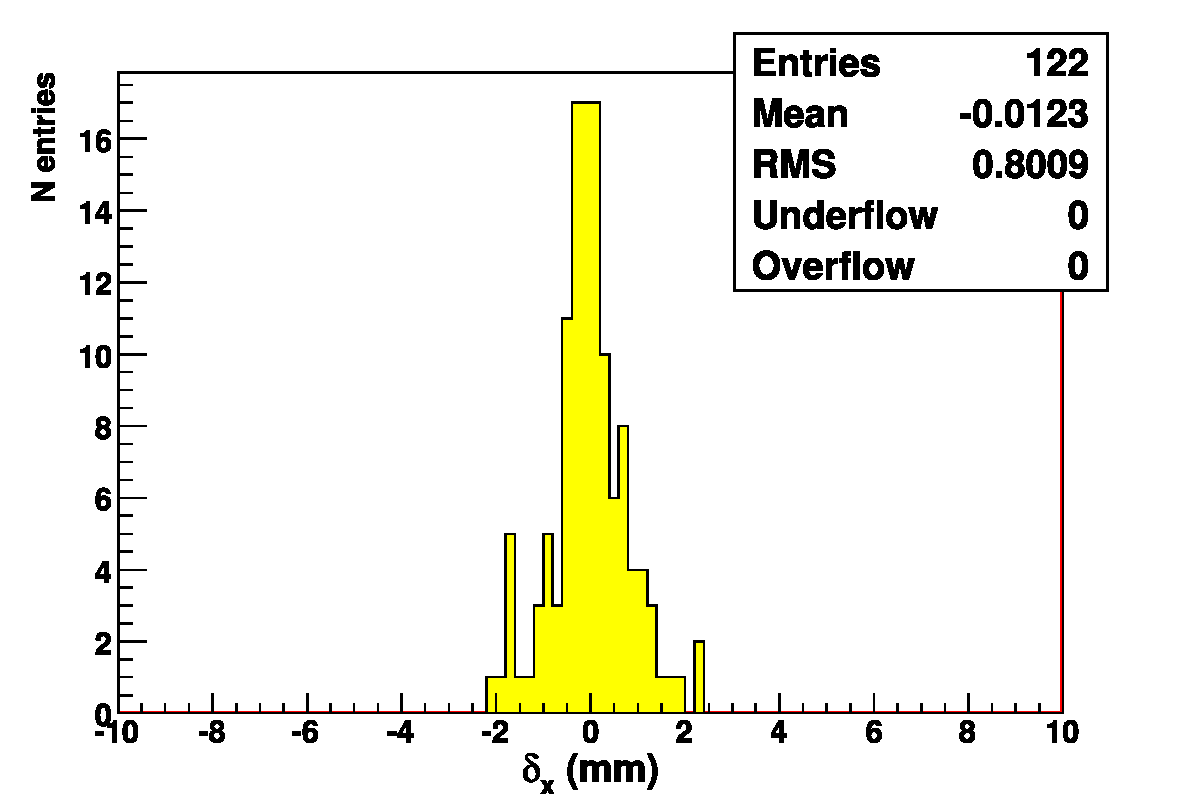
\includegraphics[width=0.32\linewidth]{plots/gma_hip_results/delta_xComparison.pdf}
%% 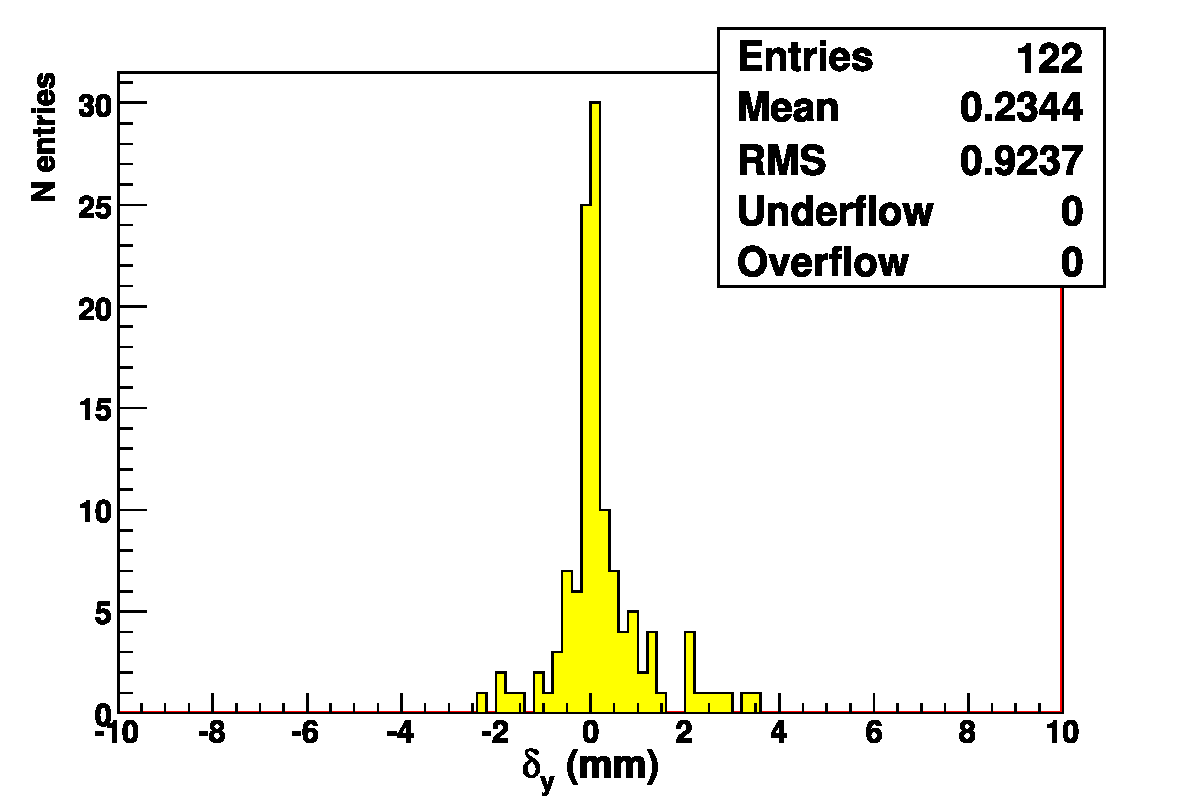
\includegraphics[width=0.32\linewidth]{plots/gma_hip_results/delta_yComparison.pdf}
%% 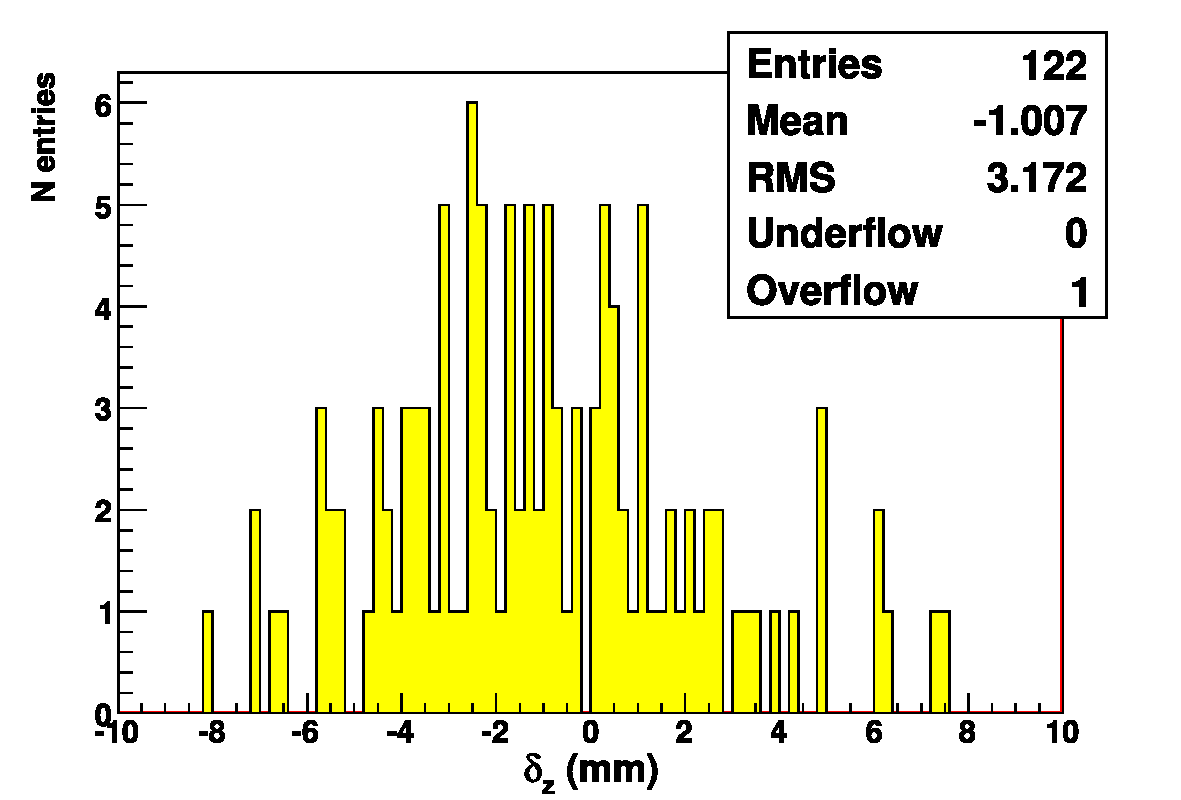
\includegraphics[width=0.32\linewidth]{plots/gma_hip_results/delta_zComparison.pdf}

%% 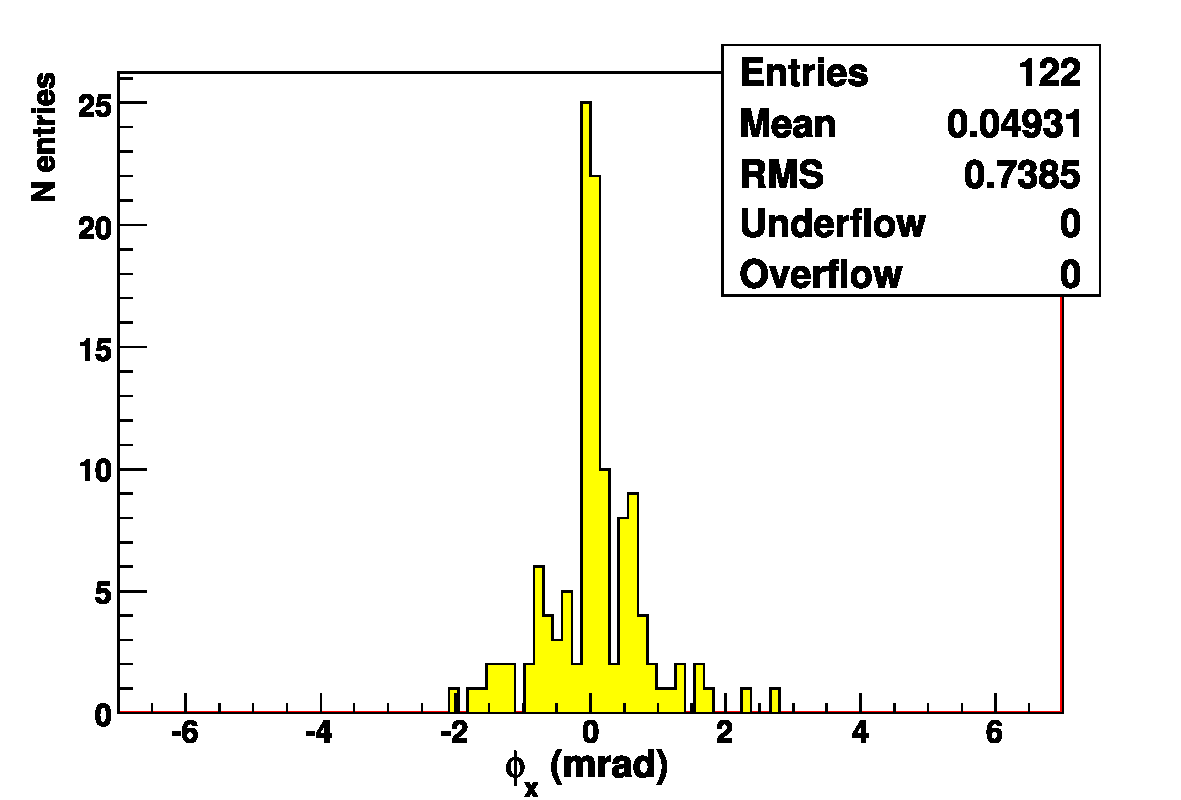
\includegraphics[width=0.32\linewidth]{plots/gma_hip_results/phixComparison.pdf}
%% 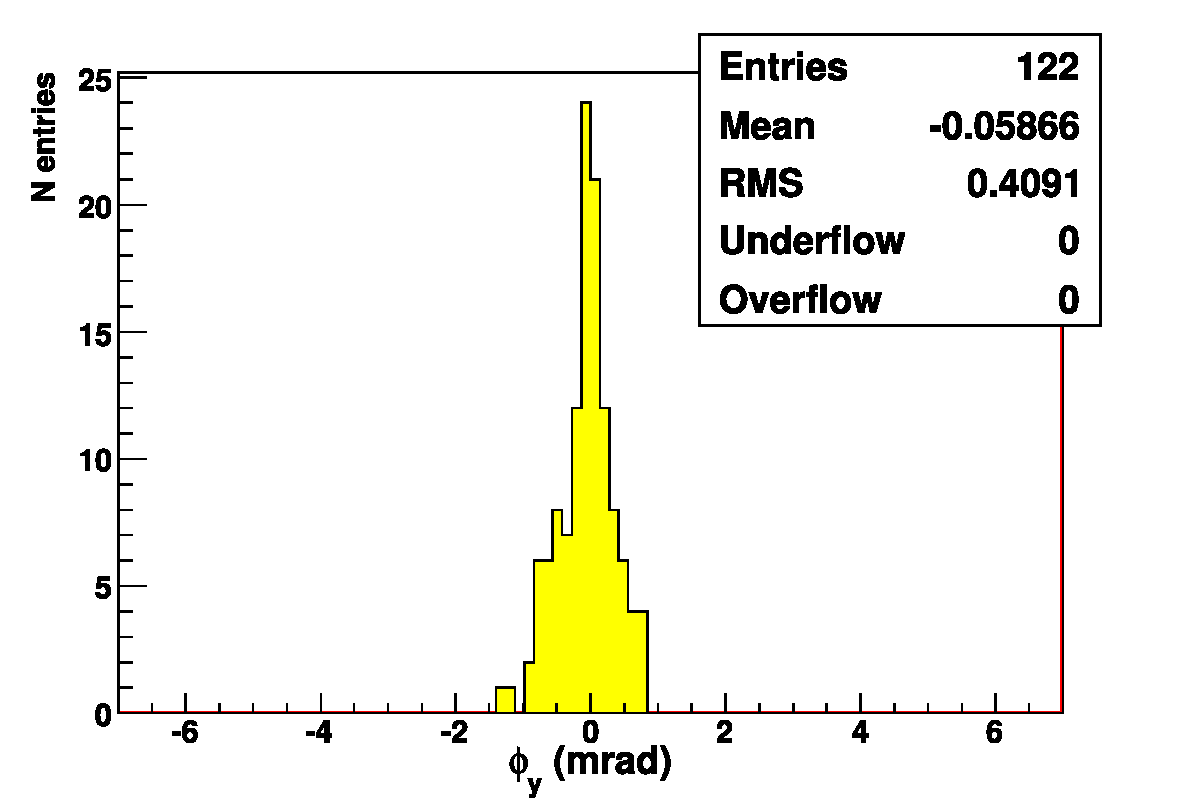
\includegraphics[width=0.32\linewidth]{plots/gma_hip_results/phiyComparison.pdf}
%% 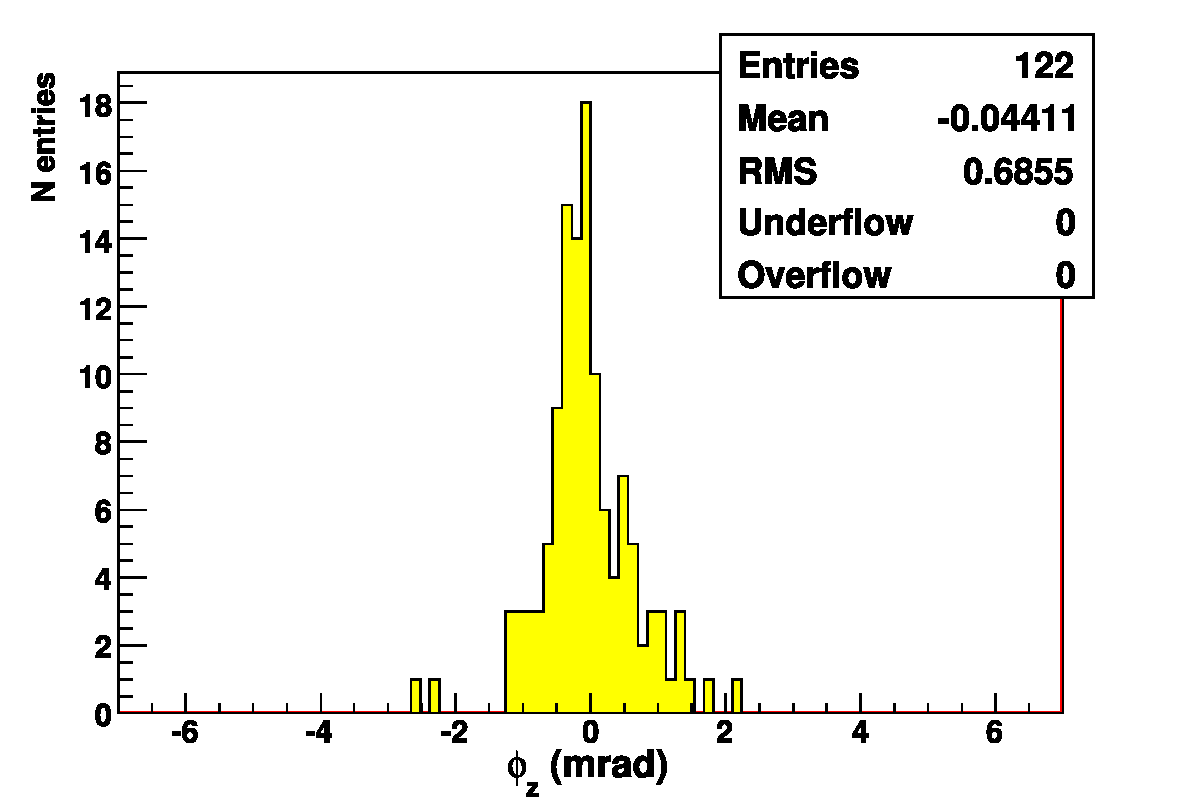
\includegraphics[width=0.32\linewidth]{plots/gma_hip_results/phizComparison.pdf}

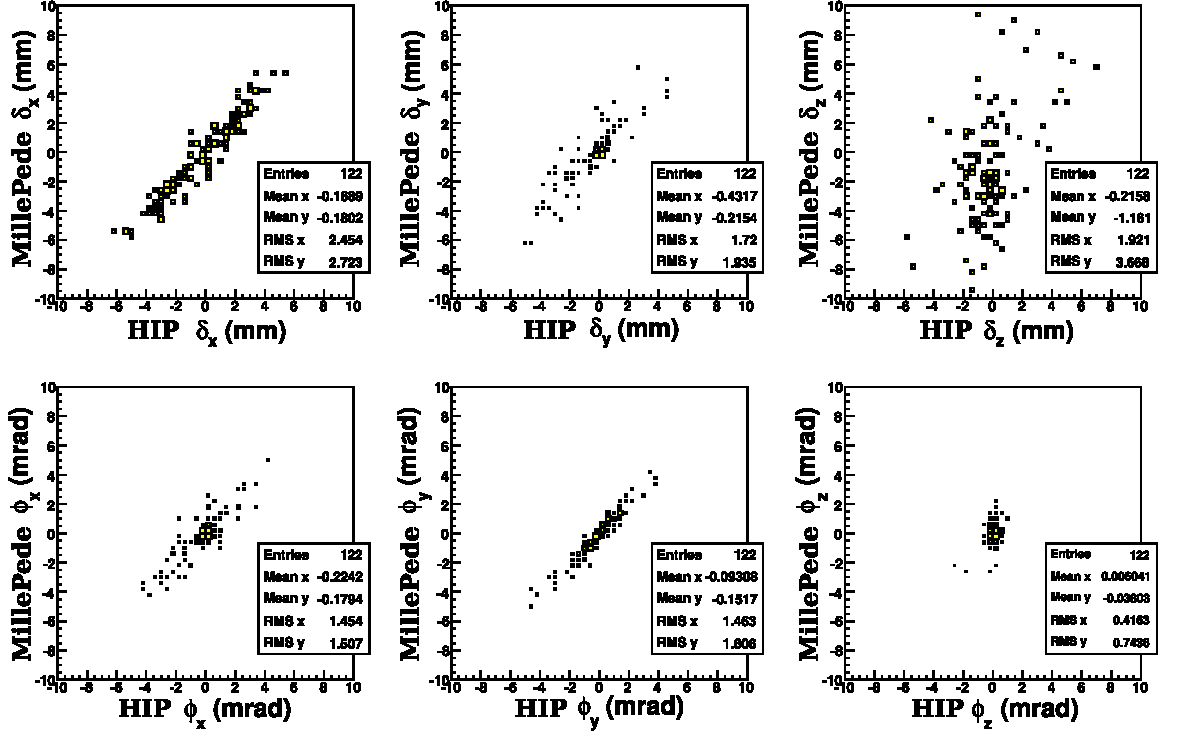
\includegraphics[width=\linewidth]{plots/gma_hip_results/MP-V4_vs_HIP-V4.pdf}
\end{center}
\caption{Alignment corrections determined by the HIP and Millepede algorithms. (Only aligned chambers are shown.)\label{fig:sidebyside}}
\end{figure}

Local alignment measurements to test consistency between global data
and local data (3) were derived by extrapolating linear track segments
from one chamber to the next (in the same sector, neighboring
stations).  This verification procedure introduces information not
used in the alignment itself, namely the higher precision with which
tracks can be propagated over a short distance (1~meter) than a long
distance (3--6~meters).

For this diagnostic, tracks were selected with $p_T > 50$~GeV and a
correction was applied to cancel the effect of the magnetic field by
taking advantage of the fact that positively- and negatively-charged
tracks are pushed in opposite directions.
%% Figure~\ref{fig:valid_DTconsts} shows the level of agreement in $x$
%% position and $\frac{dx}{dz}$ angle between segments in neighboring
%% stations for each sector in wheel~0.
To compare the initial state with the results of each algorithm in all
station-pairs, sectors, and wheels, we filled histograms with the
fitted Gaussian peak of each comparison, shown in
Figure~\ref{fig:valid_NOMvsMPvsHIP}.  Though the global algorithms
changed the positions of chambers by 2.5~mm in $\delta_x$ and 1.5~mrad
in $\delta_{\phi_y}$ (RMS in Figure~\ref{fig:sidebyside}), local
differences of 0.8--1.3~mm and 1.0--1.3~mrad are not only maintained
but reduced by 10\% to as much as a factor of 2.  As expected, the chambers which are closest
to the tracker (station~1-to-2 differences) are the most precisely
aligned.  The individual outliers in station~4 contain internal
structure in their residuals distributions which are the subject of
further study.

%% \begin{figure}
%%   \centering
%%   \subfigure[Average $x$ difference between stations]{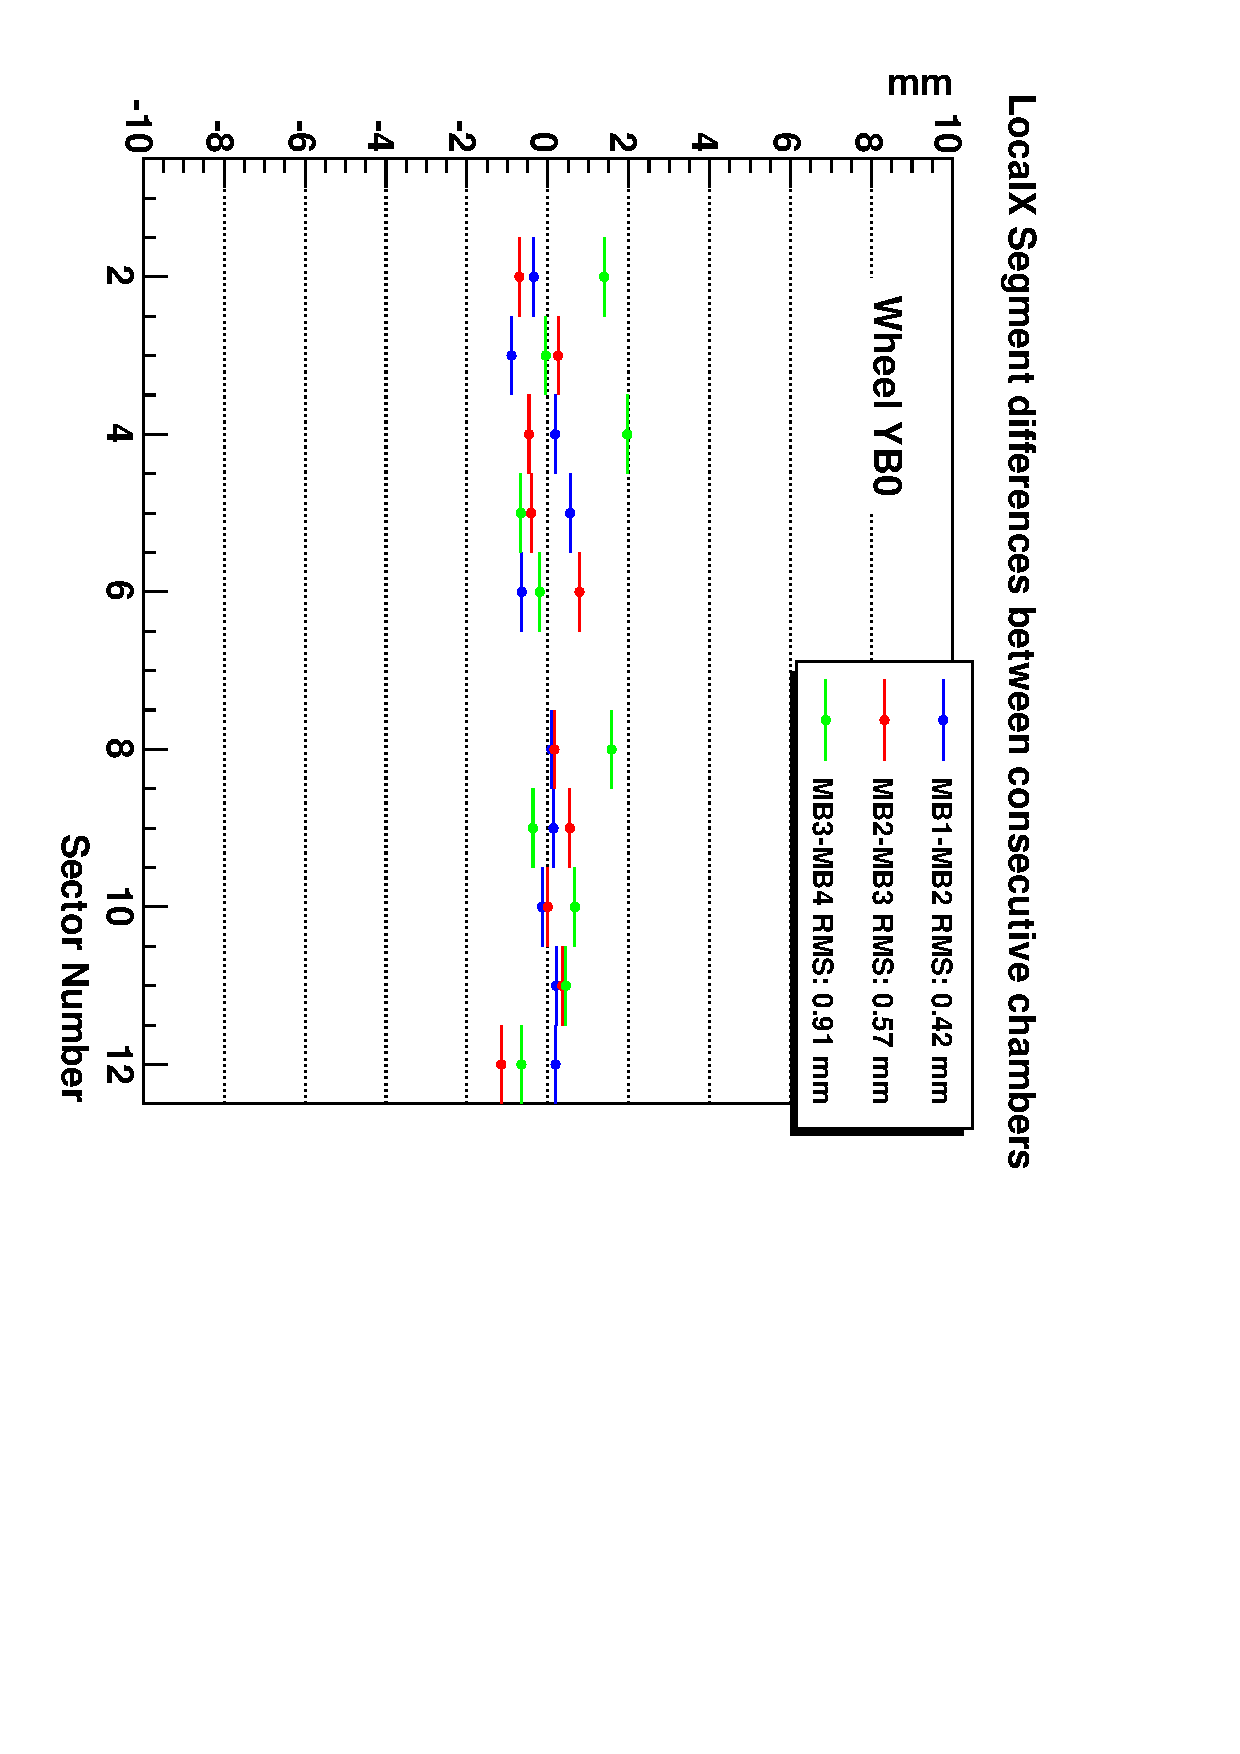
\includegraphics[width=0.4\textwidth, angle=90]{plots/validation/aligVal_08June09_LocalX_YB0.pdf}}
%%   \subfigure[Average $\frac{dx}{dz}$ difference between stations]{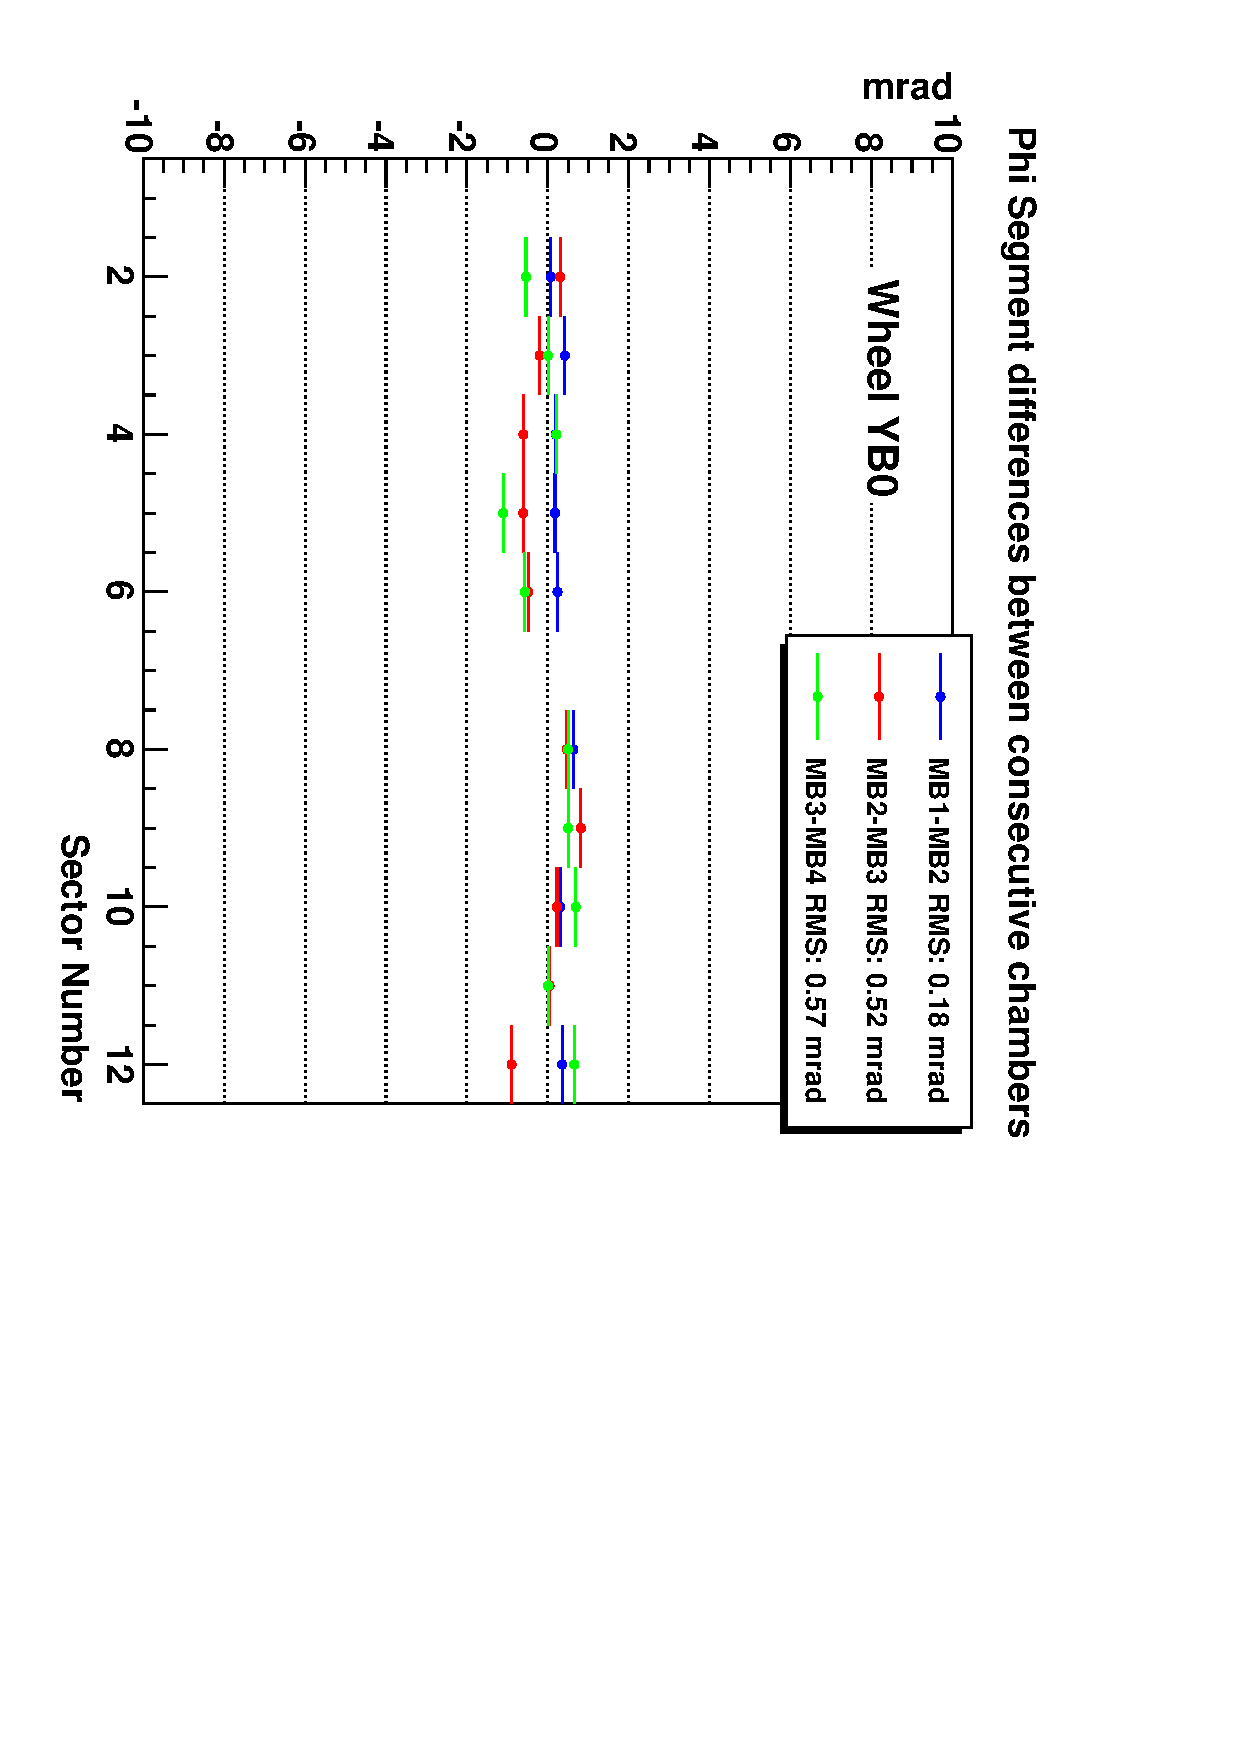
\includegraphics[width=0.4\textwidth, angle=90]{plots/validation/aligVal_08June09_Phi_YB0.pdf}}
%%   \caption{Validation of DT alignment by comparing track segments in
%%   neighboring chambers (after alignment using the HIP algorithm).\label{fig:valid_DTconsts}}
%% \end{figure}
 
\begin{figure}
  \centering
  \subfigure[Before global alignment]{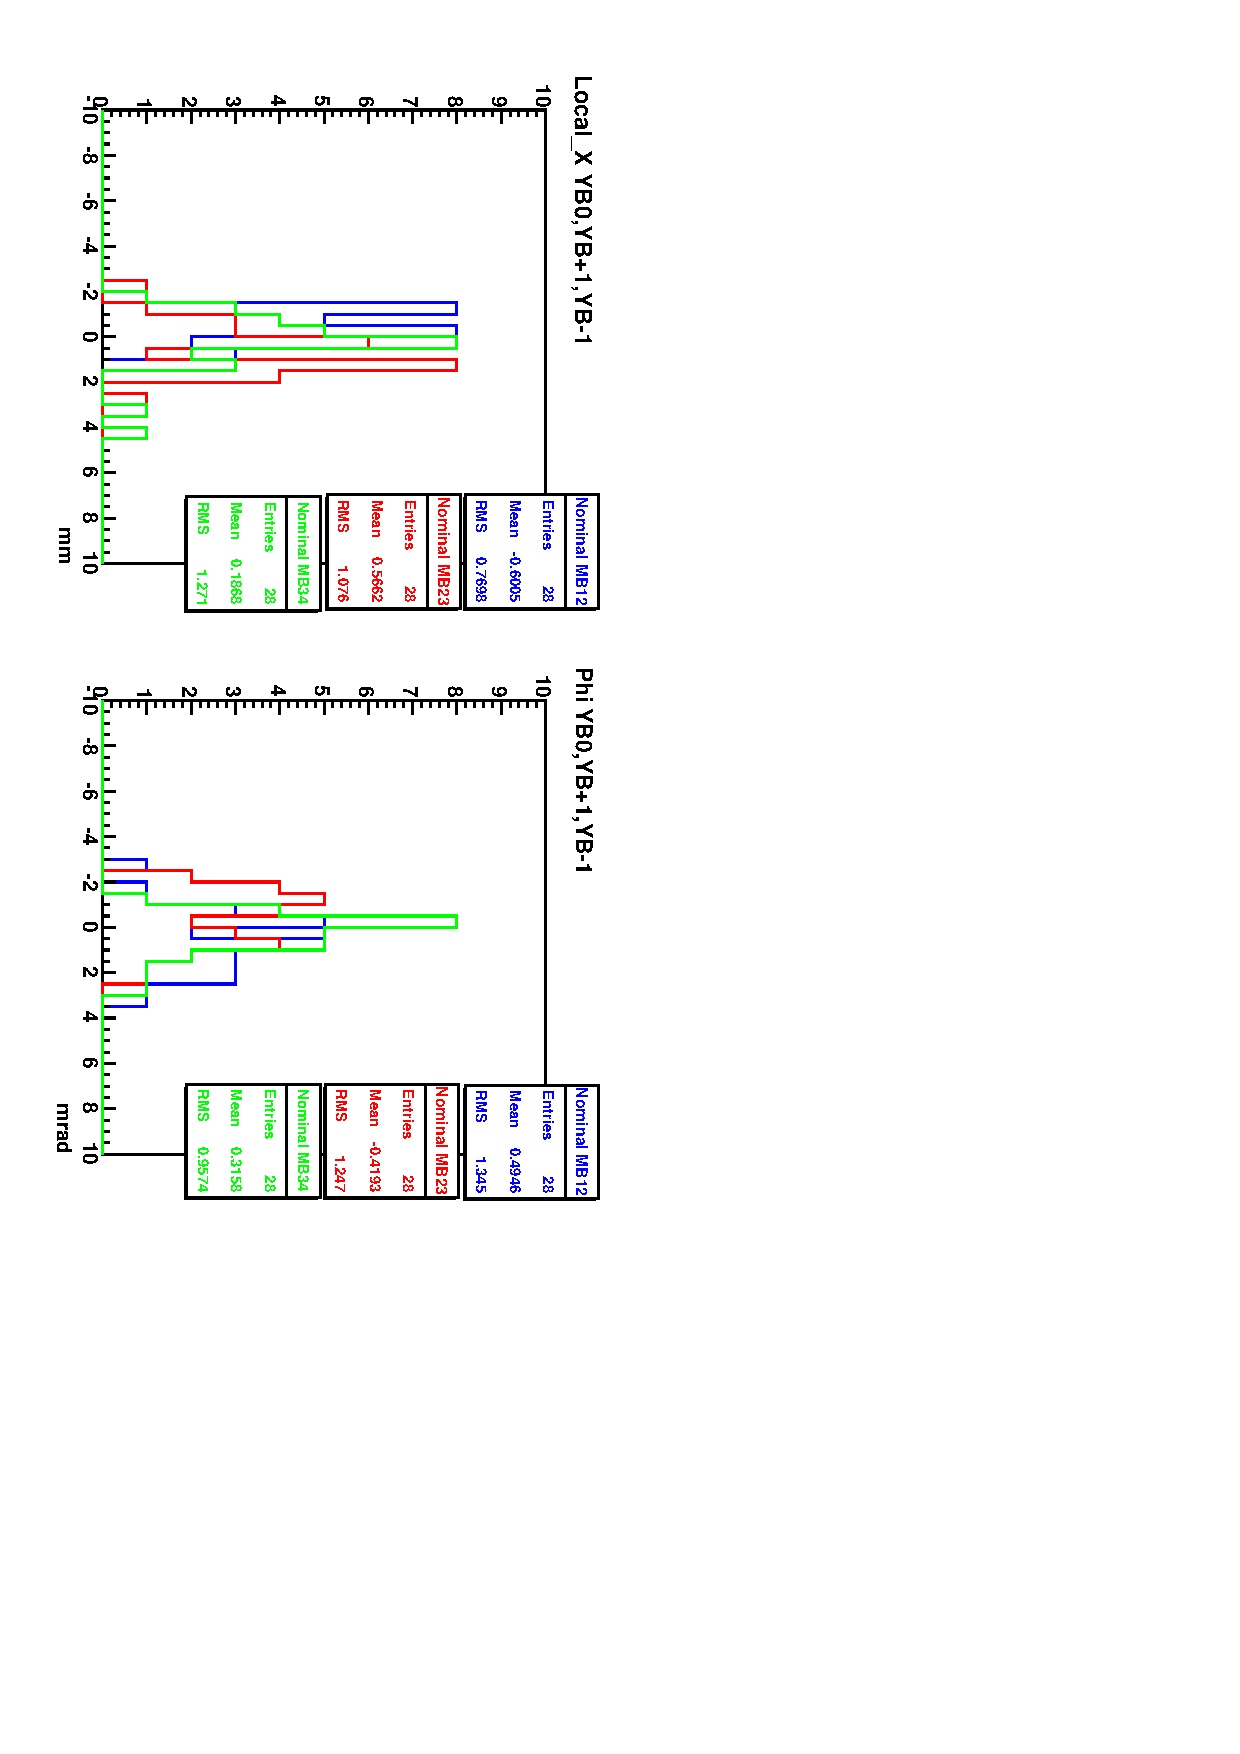
\includegraphics[width=0.4\textwidth, angle=90]{plots/gma_hip_results/YB0YB1YBm1_V4_38T.pdf}}
  \subfigure[Results from the HIP algorithm]{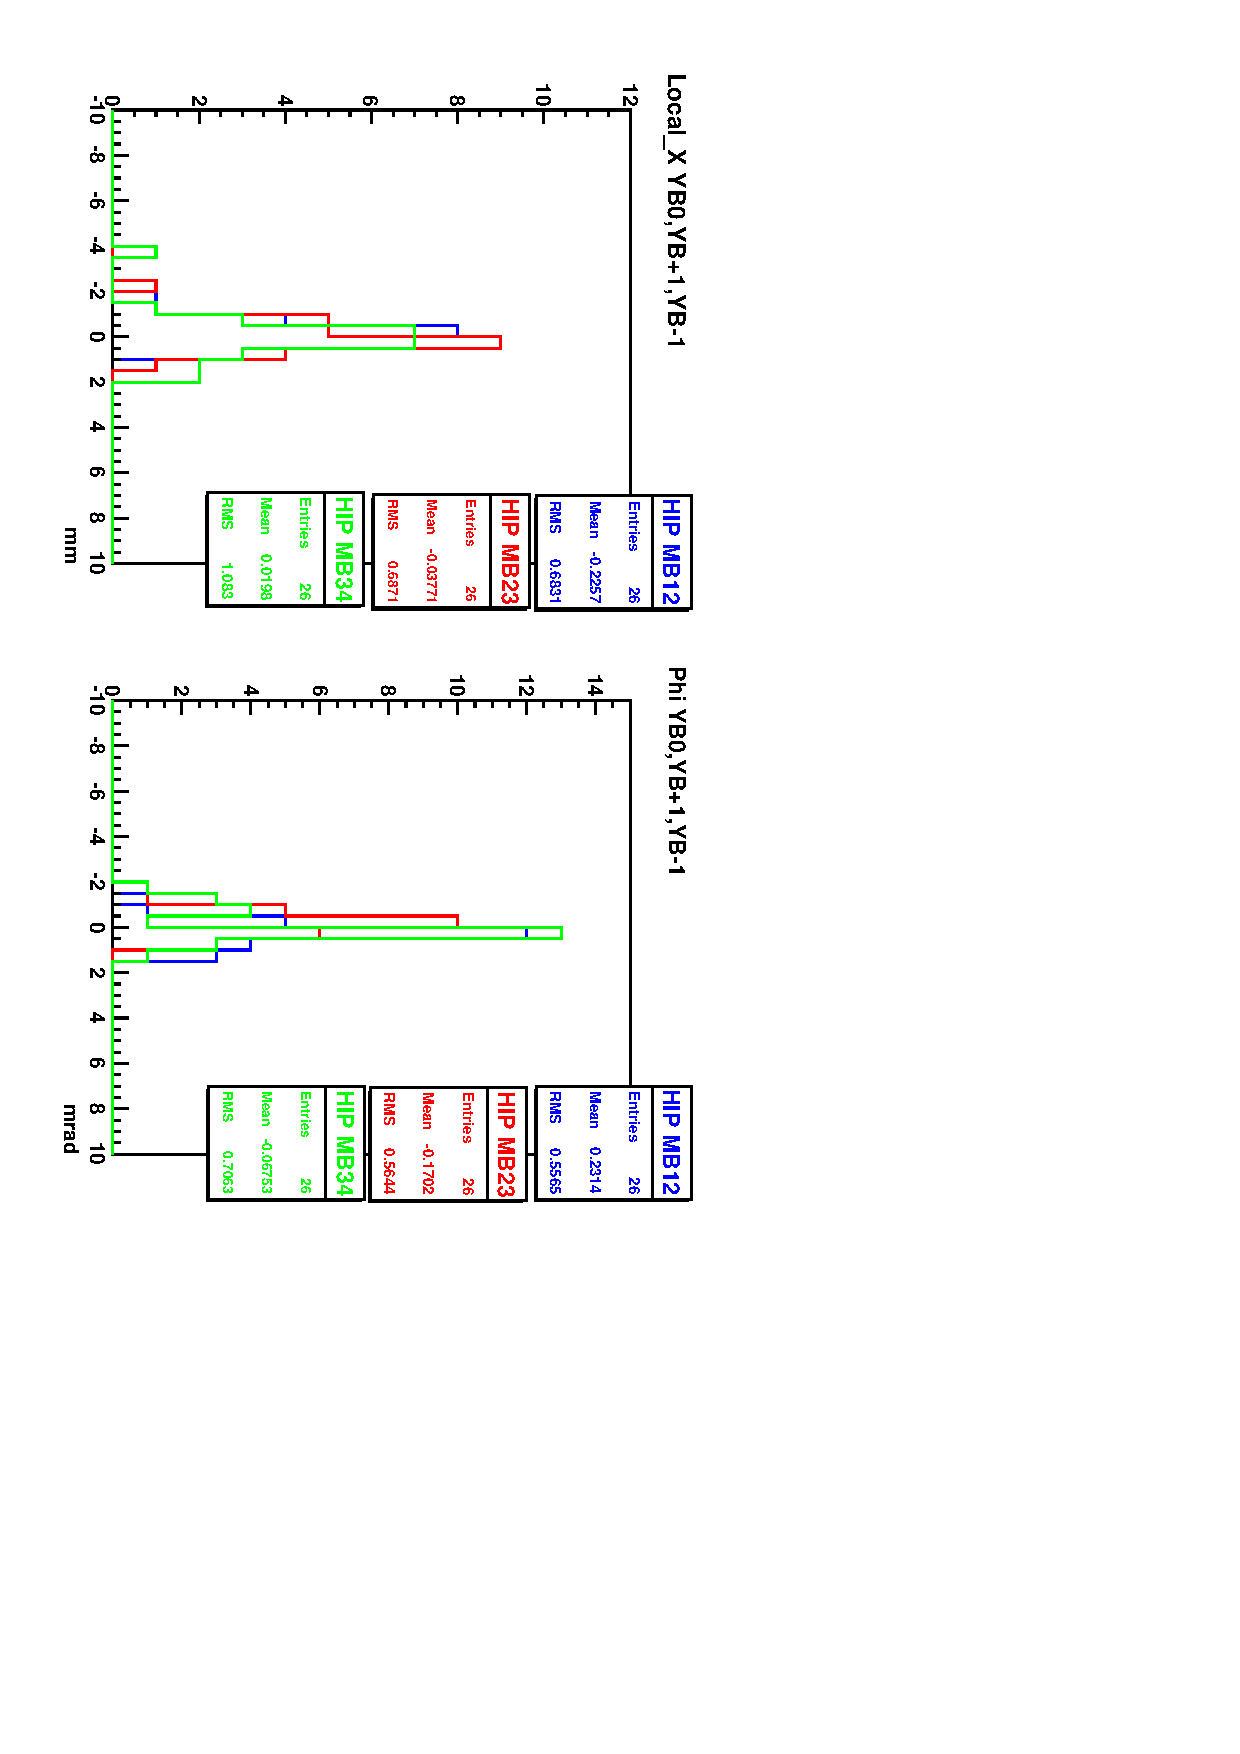
\includegraphics[width=0.45\textwidth, angle=90]{plots/validation/meanHisto_HIP_onlyAlign.pdf}}
  \subfigure[Results from the Millepede algorithm]{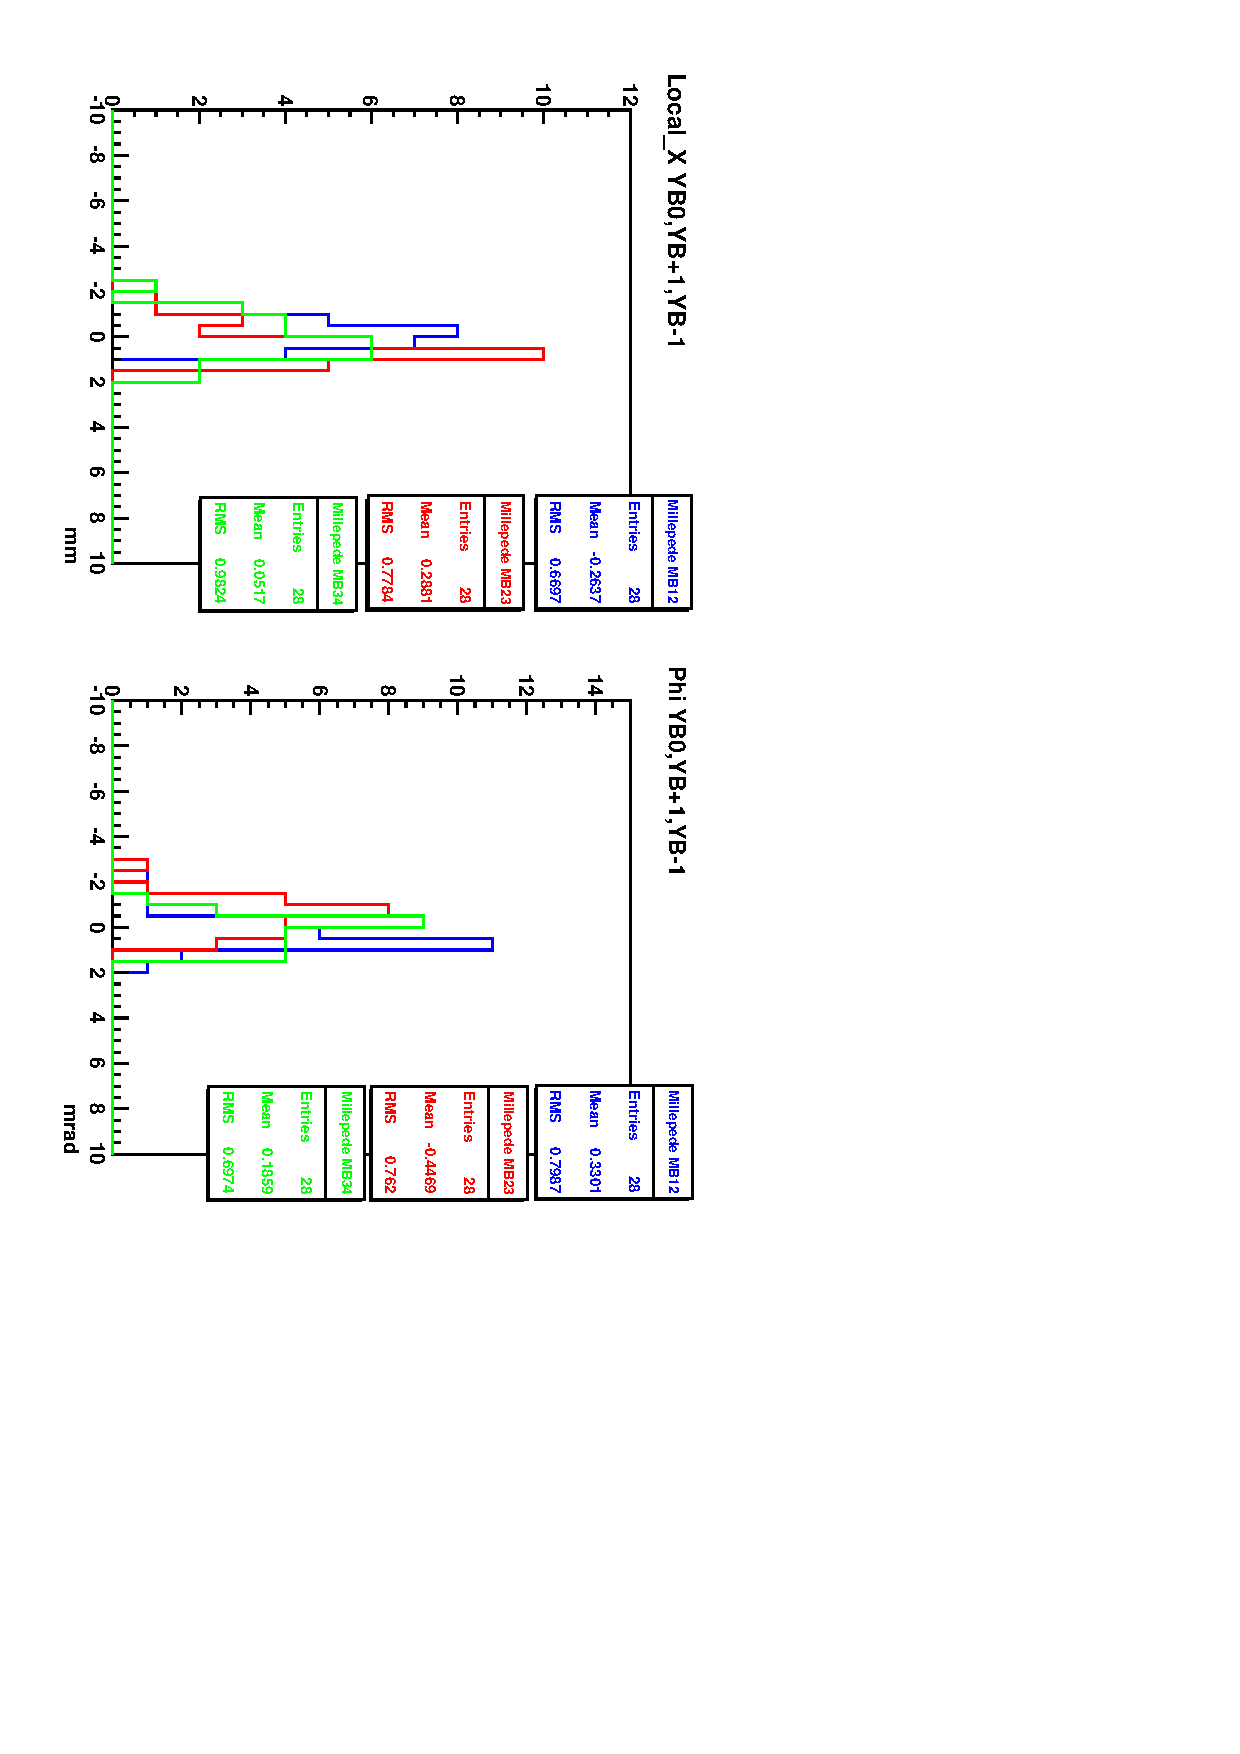
\includegraphics[width=0.45\textwidth, angle=90]{plots/validation/meanHisto_Millepede.pdf}}
  \caption{Local differences in alignment as measured by segments.  Each histogram entry is a pair of chambers in neighboring stations, but the same wheel and sector.  The three histograms show station~1-to-2 differences (blue), 2-to-3 differences (red), and 3-to-4 differences (green).  \label{fig:valid_NOMvsMPvsHIP}}
\end{figure}
 
To verify that the new alignment (in this case, HIP only) improves
momentum resolution (4), we selected cosmic rays with $p_T > 200$~GeV,
split each into two tracks near the origin (similar to what would be
observed in LHC collisions), and compared the momentum of the top and
bottom fits.  Since the cosmic ray muon is a single particle, any
mismatch between the halves is purely instrumental.  Cosmic rays have
a steeply falling distribution, so most of the selected tracks have
$p_T$ close to 200~GeV.  The alignment was performed using tracks with
$100 < p_T < 200$~GeV tracks, so the diagnostic sample is
statistically independent from the alignment.
Figure~\ref{fig:chargesplitting} compares tracker-only tracks and
tracks reconstructed with muon hits (first muon station only), before
and after the global muon alignment.

\begin{figure}
  \centering
  \subfigure[Before global muon alignment]{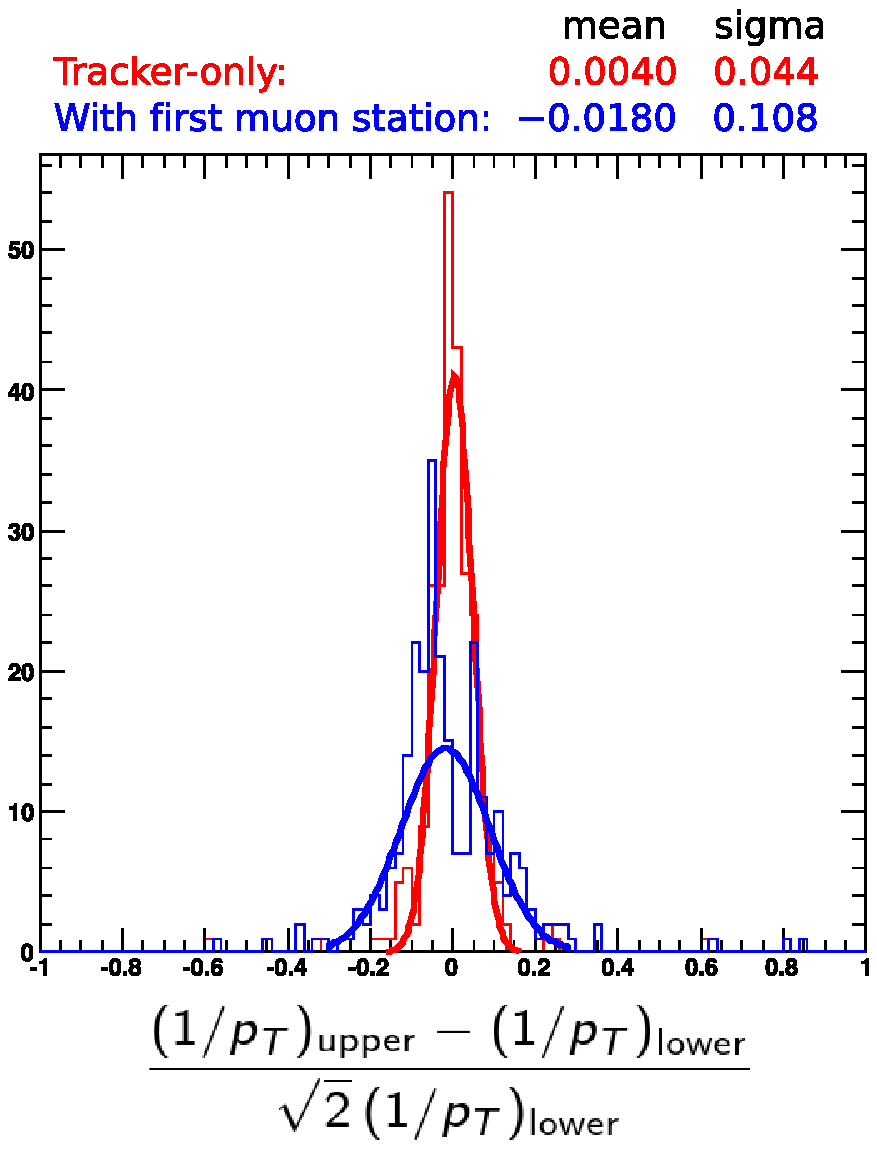
\includegraphics[width=0.45\linewidth]{plots/monitoring_validation/chargesplitting_withoutalignment.pdf}}
  \subfigure[Results from the HIP algorithm]{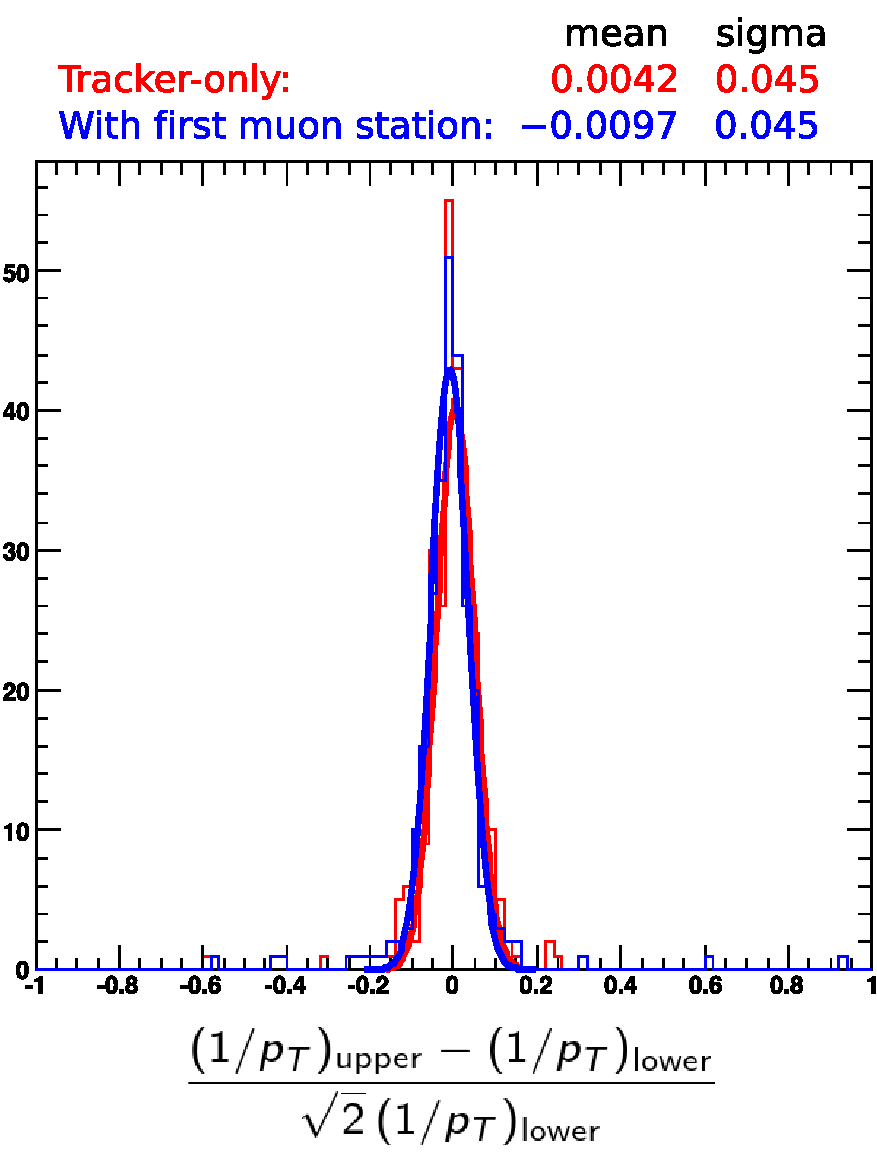
\includegraphics[width=0.45\linewidth]{plots/monitoring_validation/chargesplitting_withalignment.pdf}}
  \caption{Top vs.~bottom $1/p_T$ comparison for $p_T \gtrsim 200$~GeV split cosmic rays.\label{fig:chargesplitting}}
\end{figure}
  

%---------------------------------------------------------------------
\section{Conclusions}
In this note, we have demonstrated a variety of software procedures for
aligning different parts of the muon system: layers in DT chambers,
CSC chambers in rings, and global positions of DT chambers relative to
the central tracker, using charged tracks.  We have fully exploited the available data,
horizontal LHC beam-halo muons and vertical cosmic rays.

These procedures will be used without major modifications to re-align
the muon system with muons from LHC collisions, once such data are
available.  The azimuthally-symmetric and broad pseudorapidity
distribution of collisions muons will allow us to extend the global
alignment to all muon chambers.  Although the endcap chambers are
sensitive to only three parameters, $\delta_{r\phi}$,
$\delta_{\phi_y}$ and $\delta_{\phi_z}$ (the same as local CSC
alignment), these parameters can be determined with 400~$\mu$m,
0.4~mrad, and 0.6~mrad resolution with similar results for all degrees
of freedom in the muon barrel, according to 50~pb$^{-1}$ simulations.
To constrain the remaining CSC parameters, we can exploit the
complementarity of the endcap hardware alignment
system~\cite{ref:hardware_alignment} (which measure $\delta_z$ and
$\delta_{\phi_x}$ directly), and independently test its validity in
$\delta_{r\phi}$.

Moreover, the addition of collisions muons and larger beam-halo
datasets will allow new cross-checks to be performed, as the local CSC
alignment (section~\ref{sec:localcsc}) and CSC layer alignment can be
performed with both collisions and beam-halo, so we can doubly
cross-check by performing the same method with different track sources
and different methods with the same track source.  Similarly,
collisions and cosmic rays can both be used in the barrel, and they
differ in how the reference tracks sample the tracker, and hence
potental input track bias.

By verifying the muon alignment in as many ways as possible, we can
add confidence to the muon momentum resolution at all energy scales,
improving sensitivity to signatures of new physics.


%---------------------------------------------------------------------
\bibliography{auto_generated}   % will be created by the tdr script.

\end{document}

